\documentclass[runningheads]{llncs}

%\input{../Subfiles/Packages.tex}
% 
\subfloat[Average time (in $s$), $|\Sg| = 100$]{
	\hspace{-3em}
	\scalebox{0.44}{%% Creator: Matplotlib, PGF backend
%%
%% To include the figure in your LaTeX document, write
%%   \input{<filename>.pgf}
%%
%% Make sure the required packages are loaded in your preamble
%%   \usepackage{pgf}
%%
%% Figures using additional raster images can only be included by \input if
%% they are in the same directory as the main LaTeX file. For loading figures
%% from other directories you can use the `import` package
%%   \usepackage{import}
%% and then include the figures with
%%   \import{<path to file>}{<filename>.pgf}
%%
%% Matplotlib used the following preamble
%%   \usepackage{fontspec}
%%   \setmainfont{DejaVu Serif}
%%   \setsansfont{DejaVu Sans}
%%   \setmonofont{DejaVu Sans Mono}
%%
\begingroup%
\makeatletter%
\begin{pgfpicture}%
\pgfpathrectangle{\pgfpointorigin}{\pgfqpoint{8.100000in}{6.600000in}}%
\pgfusepath{use as bounding box, clip}%
\begin{pgfscope}%
\pgfsetbuttcap%
\pgfsetmiterjoin%
\definecolor{currentfill}{rgb}{1.000000,1.000000,1.000000}%
\pgfsetfillcolor{currentfill}%
\pgfsetlinewidth{0.000000pt}%
\definecolor{currentstroke}{rgb}{1.000000,1.000000,1.000000}%
\pgfsetstrokecolor{currentstroke}%
\pgfsetdash{}{0pt}%
\pgfpathmoveto{\pgfqpoint{0.000000in}{0.000000in}}%
\pgfpathlineto{\pgfqpoint{8.100000in}{0.000000in}}%
\pgfpathlineto{\pgfqpoint{8.100000in}{6.600000in}}%
\pgfpathlineto{\pgfqpoint{0.000000in}{6.600000in}}%
\pgfpathclose%
\pgfusepath{fill}%
\end{pgfscope}%
\begin{pgfscope}%
\pgfsetbuttcap%
\pgfsetmiterjoin%
\definecolor{currentfill}{rgb}{1.000000,1.000000,1.000000}%
\pgfsetfillcolor{currentfill}%
\pgfsetlinewidth{0.000000pt}%
\definecolor{currentstroke}{rgb}{0.000000,0.000000,0.000000}%
\pgfsetstrokecolor{currentstroke}%
\pgfsetstrokeopacity{0.000000}%
\pgfsetdash{}{0pt}%
\pgfpathmoveto{\pgfqpoint{1.012500in}{0.726000in}}%
\pgfpathlineto{\pgfqpoint{7.290000in}{0.726000in}}%
\pgfpathlineto{\pgfqpoint{7.290000in}{5.808000in}}%
\pgfpathlineto{\pgfqpoint{1.012500in}{5.808000in}}%
\pgfpathclose%
\pgfusepath{fill}%
\end{pgfscope}%
\begin{pgfscope}%
\pgfsetbuttcap%
\pgfsetroundjoin%
\definecolor{currentfill}{rgb}{0.000000,0.000000,0.000000}%
\pgfsetfillcolor{currentfill}%
\pgfsetlinewidth{0.803000pt}%
\definecolor{currentstroke}{rgb}{0.000000,0.000000,0.000000}%
\pgfsetstrokecolor{currentstroke}%
\pgfsetdash{}{0pt}%
\pgfsys@defobject{currentmarker}{\pgfqpoint{0.000000in}{-0.048611in}}{\pgfqpoint{0.000000in}{0.000000in}}{%
\pgfpathmoveto{\pgfqpoint{0.000000in}{0.000000in}}%
\pgfpathlineto{\pgfqpoint{0.000000in}{-0.048611in}}%
\pgfusepath{stroke,fill}%
}%
\begin{pgfscope}%
\pgfsys@transformshift{1.012500in}{0.726000in}%
\pgfsys@useobject{currentmarker}{}%
\end{pgfscope}%
\end{pgfscope}%
\begin{pgfscope}%
\pgftext[x=1.012500in,y=0.628778in,,top]{\sffamily\fontsize{10.000000}{12.000000}\selectfont \(\displaystyle 0\)}%
\end{pgfscope}%
\begin{pgfscope}%
\pgfsetbuttcap%
\pgfsetroundjoin%
\definecolor{currentfill}{rgb}{0.000000,0.000000,0.000000}%
\pgfsetfillcolor{currentfill}%
\pgfsetlinewidth{0.803000pt}%
\definecolor{currentstroke}{rgb}{0.000000,0.000000,0.000000}%
\pgfsetstrokecolor{currentstroke}%
\pgfsetdash{}{0pt}%
\pgfsys@defobject{currentmarker}{\pgfqpoint{0.000000in}{-0.048611in}}{\pgfqpoint{0.000000in}{0.000000in}}{%
\pgfpathmoveto{\pgfqpoint{0.000000in}{0.000000in}}%
\pgfpathlineto{\pgfqpoint{0.000000in}{-0.048611in}}%
\pgfusepath{stroke,fill}%
}%
\begin{pgfscope}%
\pgfsys@transformshift{1.611784in}{0.726000in}%
\pgfsys@useobject{currentmarker}{}%
\end{pgfscope}%
\end{pgfscope}%
\begin{pgfscope}%
\pgftext[x=1.611784in,y=0.628778in,,top]{\sffamily\fontsize{10.000000}{12.000000}\selectfont \(\displaystyle 2000\)}%
\end{pgfscope}%
\begin{pgfscope}%
\pgfsetbuttcap%
\pgfsetroundjoin%
\definecolor{currentfill}{rgb}{0.000000,0.000000,0.000000}%
\pgfsetfillcolor{currentfill}%
\pgfsetlinewidth{0.803000pt}%
\definecolor{currentstroke}{rgb}{0.000000,0.000000,0.000000}%
\pgfsetstrokecolor{currentstroke}%
\pgfsetdash{}{0pt}%
\pgfsys@defobject{currentmarker}{\pgfqpoint{0.000000in}{-0.048611in}}{\pgfqpoint{0.000000in}{0.000000in}}{%
\pgfpathmoveto{\pgfqpoint{0.000000in}{0.000000in}}%
\pgfpathlineto{\pgfqpoint{0.000000in}{-0.048611in}}%
\pgfusepath{stroke,fill}%
}%
\begin{pgfscope}%
\pgfsys@transformshift{2.211068in}{0.726000in}%
\pgfsys@useobject{currentmarker}{}%
\end{pgfscope}%
\end{pgfscope}%
\begin{pgfscope}%
\pgftext[x=2.211068in,y=0.628778in,,top]{\sffamily\fontsize{10.000000}{12.000000}\selectfont \(\displaystyle 4000\)}%
\end{pgfscope}%
\begin{pgfscope}%
\pgfsetbuttcap%
\pgfsetroundjoin%
\definecolor{currentfill}{rgb}{0.000000,0.000000,0.000000}%
\pgfsetfillcolor{currentfill}%
\pgfsetlinewidth{0.803000pt}%
\definecolor{currentstroke}{rgb}{0.000000,0.000000,0.000000}%
\pgfsetstrokecolor{currentstroke}%
\pgfsetdash{}{0pt}%
\pgfsys@defobject{currentmarker}{\pgfqpoint{0.000000in}{-0.048611in}}{\pgfqpoint{0.000000in}{0.000000in}}{%
\pgfpathmoveto{\pgfqpoint{0.000000in}{0.000000in}}%
\pgfpathlineto{\pgfqpoint{0.000000in}{-0.048611in}}%
\pgfusepath{stroke,fill}%
}%
\begin{pgfscope}%
\pgfsys@transformshift{2.810352in}{0.726000in}%
\pgfsys@useobject{currentmarker}{}%
\end{pgfscope}%
\end{pgfscope}%
\begin{pgfscope}%
\pgftext[x=2.810352in,y=0.628778in,,top]{\sffamily\fontsize{10.000000}{12.000000}\selectfont \(\displaystyle 6000\)}%
\end{pgfscope}%
\begin{pgfscope}%
\pgfsetbuttcap%
\pgfsetroundjoin%
\definecolor{currentfill}{rgb}{0.000000,0.000000,0.000000}%
\pgfsetfillcolor{currentfill}%
\pgfsetlinewidth{0.803000pt}%
\definecolor{currentstroke}{rgb}{0.000000,0.000000,0.000000}%
\pgfsetstrokecolor{currentstroke}%
\pgfsetdash{}{0pt}%
\pgfsys@defobject{currentmarker}{\pgfqpoint{0.000000in}{-0.048611in}}{\pgfqpoint{0.000000in}{0.000000in}}{%
\pgfpathmoveto{\pgfqpoint{0.000000in}{0.000000in}}%
\pgfpathlineto{\pgfqpoint{0.000000in}{-0.048611in}}%
\pgfusepath{stroke,fill}%
}%
\begin{pgfscope}%
\pgfsys@transformshift{3.409636in}{0.726000in}%
\pgfsys@useobject{currentmarker}{}%
\end{pgfscope}%
\end{pgfscope}%
\begin{pgfscope}%
\pgftext[x=3.409636in,y=0.628778in,,top]{\sffamily\fontsize{10.000000}{12.000000}\selectfont \(\displaystyle 8000\)}%
\end{pgfscope}%
\begin{pgfscope}%
\pgfsetbuttcap%
\pgfsetroundjoin%
\definecolor{currentfill}{rgb}{0.000000,0.000000,0.000000}%
\pgfsetfillcolor{currentfill}%
\pgfsetlinewidth{0.803000pt}%
\definecolor{currentstroke}{rgb}{0.000000,0.000000,0.000000}%
\pgfsetstrokecolor{currentstroke}%
\pgfsetdash{}{0pt}%
\pgfsys@defobject{currentmarker}{\pgfqpoint{0.000000in}{-0.048611in}}{\pgfqpoint{0.000000in}{0.000000in}}{%
\pgfpathmoveto{\pgfqpoint{0.000000in}{0.000000in}}%
\pgfpathlineto{\pgfqpoint{0.000000in}{-0.048611in}}%
\pgfusepath{stroke,fill}%
}%
\begin{pgfscope}%
\pgfsys@transformshift{4.008920in}{0.726000in}%
\pgfsys@useobject{currentmarker}{}%
\end{pgfscope}%
\end{pgfscope}%
\begin{pgfscope}%
\pgftext[x=4.008920in,y=0.628778in,,top]{\sffamily\fontsize{10.000000}{12.000000}\selectfont \(\displaystyle 10000\)}%
\end{pgfscope}%
\begin{pgfscope}%
\pgfsetbuttcap%
\pgfsetroundjoin%
\definecolor{currentfill}{rgb}{0.000000,0.000000,0.000000}%
\pgfsetfillcolor{currentfill}%
\pgfsetlinewidth{0.803000pt}%
\definecolor{currentstroke}{rgb}{0.000000,0.000000,0.000000}%
\pgfsetstrokecolor{currentstroke}%
\pgfsetdash{}{0pt}%
\pgfsys@defobject{currentmarker}{\pgfqpoint{0.000000in}{-0.048611in}}{\pgfqpoint{0.000000in}{0.000000in}}{%
\pgfpathmoveto{\pgfqpoint{0.000000in}{0.000000in}}%
\pgfpathlineto{\pgfqpoint{0.000000in}{-0.048611in}}%
\pgfusepath{stroke,fill}%
}%
\begin{pgfscope}%
\pgfsys@transformshift{4.608204in}{0.726000in}%
\pgfsys@useobject{currentmarker}{}%
\end{pgfscope}%
\end{pgfscope}%
\begin{pgfscope}%
\pgftext[x=4.608204in,y=0.628778in,,top]{\sffamily\fontsize{10.000000}{12.000000}\selectfont \(\displaystyle 12000\)}%
\end{pgfscope}%
\begin{pgfscope}%
\pgfsetbuttcap%
\pgfsetroundjoin%
\definecolor{currentfill}{rgb}{0.000000,0.000000,0.000000}%
\pgfsetfillcolor{currentfill}%
\pgfsetlinewidth{0.803000pt}%
\definecolor{currentstroke}{rgb}{0.000000,0.000000,0.000000}%
\pgfsetstrokecolor{currentstroke}%
\pgfsetdash{}{0pt}%
\pgfsys@defobject{currentmarker}{\pgfqpoint{0.000000in}{-0.048611in}}{\pgfqpoint{0.000000in}{0.000000in}}{%
\pgfpathmoveto{\pgfqpoint{0.000000in}{0.000000in}}%
\pgfpathlineto{\pgfqpoint{0.000000in}{-0.048611in}}%
\pgfusepath{stroke,fill}%
}%
\begin{pgfscope}%
\pgfsys@transformshift{5.207488in}{0.726000in}%
\pgfsys@useobject{currentmarker}{}%
\end{pgfscope}%
\end{pgfscope}%
\begin{pgfscope}%
\pgftext[x=5.207488in,y=0.628778in,,top]{\sffamily\fontsize{10.000000}{12.000000}\selectfont \(\displaystyle 14000\)}%
\end{pgfscope}%
\begin{pgfscope}%
\pgfsetbuttcap%
\pgfsetroundjoin%
\definecolor{currentfill}{rgb}{0.000000,0.000000,0.000000}%
\pgfsetfillcolor{currentfill}%
\pgfsetlinewidth{0.803000pt}%
\definecolor{currentstroke}{rgb}{0.000000,0.000000,0.000000}%
\pgfsetstrokecolor{currentstroke}%
\pgfsetdash{}{0pt}%
\pgfsys@defobject{currentmarker}{\pgfqpoint{0.000000in}{-0.048611in}}{\pgfqpoint{0.000000in}{0.000000in}}{%
\pgfpathmoveto{\pgfqpoint{0.000000in}{0.000000in}}%
\pgfpathlineto{\pgfqpoint{0.000000in}{-0.048611in}}%
\pgfusepath{stroke,fill}%
}%
\begin{pgfscope}%
\pgfsys@transformshift{5.806772in}{0.726000in}%
\pgfsys@useobject{currentmarker}{}%
\end{pgfscope}%
\end{pgfscope}%
\begin{pgfscope}%
\pgftext[x=5.806772in,y=0.628778in,,top]{\sffamily\fontsize{10.000000}{12.000000}\selectfont \(\displaystyle 16000\)}%
\end{pgfscope}%
\begin{pgfscope}%
\pgfsetbuttcap%
\pgfsetroundjoin%
\definecolor{currentfill}{rgb}{0.000000,0.000000,0.000000}%
\pgfsetfillcolor{currentfill}%
\pgfsetlinewidth{0.803000pt}%
\definecolor{currentstroke}{rgb}{0.000000,0.000000,0.000000}%
\pgfsetstrokecolor{currentstroke}%
\pgfsetdash{}{0pt}%
\pgfsys@defobject{currentmarker}{\pgfqpoint{0.000000in}{-0.048611in}}{\pgfqpoint{0.000000in}{0.000000in}}{%
\pgfpathmoveto{\pgfqpoint{0.000000in}{0.000000in}}%
\pgfpathlineto{\pgfqpoint{0.000000in}{-0.048611in}}%
\pgfusepath{stroke,fill}%
}%
\begin{pgfscope}%
\pgfsys@transformshift{6.406056in}{0.726000in}%
\pgfsys@useobject{currentmarker}{}%
\end{pgfscope}%
\end{pgfscope}%
\begin{pgfscope}%
\pgftext[x=6.406056in,y=0.628778in,,top]{\sffamily\fontsize{10.000000}{12.000000}\selectfont \(\displaystyle 18000\)}%
\end{pgfscope}%
\begin{pgfscope}%
\pgfsetbuttcap%
\pgfsetroundjoin%
\definecolor{currentfill}{rgb}{0.000000,0.000000,0.000000}%
\pgfsetfillcolor{currentfill}%
\pgfsetlinewidth{0.803000pt}%
\definecolor{currentstroke}{rgb}{0.000000,0.000000,0.000000}%
\pgfsetstrokecolor{currentstroke}%
\pgfsetdash{}{0pt}%
\pgfsys@defobject{currentmarker}{\pgfqpoint{0.000000in}{-0.048611in}}{\pgfqpoint{0.000000in}{0.000000in}}{%
\pgfpathmoveto{\pgfqpoint{0.000000in}{0.000000in}}%
\pgfpathlineto{\pgfqpoint{0.000000in}{-0.048611in}}%
\pgfusepath{stroke,fill}%
}%
\begin{pgfscope}%
\pgfsys@transformshift{7.005340in}{0.726000in}%
\pgfsys@useobject{currentmarker}{}%
\end{pgfscope}%
\end{pgfscope}%
\begin{pgfscope}%
\pgftext[x=7.005340in,y=0.628778in,,top]{\sffamily\fontsize{10.000000}{12.000000}\selectfont \(\displaystyle 20000\)}%
\end{pgfscope}%
\begin{pgfscope}%
\pgftext[x=4.151250in,y=0.438809in,,top]{\sffamily\fontsize{12.000000}{14.400000}\selectfont \(\displaystyle |\mathcal{B}|\)}%
\end{pgfscope}%
\begin{pgfscope}%
\pgfsetbuttcap%
\pgfsetroundjoin%
\definecolor{currentfill}{rgb}{0.000000,0.000000,0.000000}%
\pgfsetfillcolor{currentfill}%
\pgfsetlinewidth{0.803000pt}%
\definecolor{currentstroke}{rgb}{0.000000,0.000000,0.000000}%
\pgfsetstrokecolor{currentstroke}%
\pgfsetdash{}{0pt}%
\pgfsys@defobject{currentmarker}{\pgfqpoint{-0.048611in}{0.000000in}}{\pgfqpoint{0.000000in}{0.000000in}}{%
\pgfpathmoveto{\pgfqpoint{0.000000in}{0.000000in}}%
\pgfpathlineto{\pgfqpoint{-0.048611in}{0.000000in}}%
\pgfusepath{stroke,fill}%
}%
\begin{pgfscope}%
\pgfsys@transformshift{1.012500in}{0.956312in}%
\pgfsys@useobject{currentmarker}{}%
\end{pgfscope}%
\end{pgfscope}%
\begin{pgfscope}%
\pgftext[x=0.845833in,y=0.903550in,left,base]{\sffamily\fontsize{10.000000}{12.000000}\selectfont \(\displaystyle 0\)}%
\end{pgfscope}%
\begin{pgfscope}%
\pgfsetbuttcap%
\pgfsetroundjoin%
\definecolor{currentfill}{rgb}{0.000000,0.000000,0.000000}%
\pgfsetfillcolor{currentfill}%
\pgfsetlinewidth{0.803000pt}%
\definecolor{currentstroke}{rgb}{0.000000,0.000000,0.000000}%
\pgfsetstrokecolor{currentstroke}%
\pgfsetdash{}{0pt}%
\pgfsys@defobject{currentmarker}{\pgfqpoint{-0.048611in}{0.000000in}}{\pgfqpoint{0.000000in}{0.000000in}}{%
\pgfpathmoveto{\pgfqpoint{0.000000in}{0.000000in}}%
\pgfpathlineto{\pgfqpoint{-0.048611in}{0.000000in}}%
\pgfusepath{stroke,fill}%
}%
\begin{pgfscope}%
\pgfsys@transformshift{1.012500in}{1.163097in}%
\pgfsys@useobject{currentmarker}{}%
\end{pgfscope}%
\end{pgfscope}%
\begin{pgfscope}%
\pgftext[x=0.776388in,y=1.110336in,left,base]{\sffamily\fontsize{10.000000}{12.000000}\selectfont \(\displaystyle 10\)}%
\end{pgfscope}%
\begin{pgfscope}%
\pgfsetbuttcap%
\pgfsetroundjoin%
\definecolor{currentfill}{rgb}{0.000000,0.000000,0.000000}%
\pgfsetfillcolor{currentfill}%
\pgfsetlinewidth{0.803000pt}%
\definecolor{currentstroke}{rgb}{0.000000,0.000000,0.000000}%
\pgfsetstrokecolor{currentstroke}%
\pgfsetdash{}{0pt}%
\pgfsys@defobject{currentmarker}{\pgfqpoint{-0.048611in}{0.000000in}}{\pgfqpoint{0.000000in}{0.000000in}}{%
\pgfpathmoveto{\pgfqpoint{0.000000in}{0.000000in}}%
\pgfpathlineto{\pgfqpoint{-0.048611in}{0.000000in}}%
\pgfusepath{stroke,fill}%
}%
\begin{pgfscope}%
\pgfsys@transformshift{1.012500in}{1.369883in}%
\pgfsys@useobject{currentmarker}{}%
\end{pgfscope}%
\end{pgfscope}%
\begin{pgfscope}%
\pgftext[x=0.776388in,y=1.317122in,left,base]{\sffamily\fontsize{10.000000}{12.000000}\selectfont \(\displaystyle 20\)}%
\end{pgfscope}%
\begin{pgfscope}%
\pgfsetbuttcap%
\pgfsetroundjoin%
\definecolor{currentfill}{rgb}{0.000000,0.000000,0.000000}%
\pgfsetfillcolor{currentfill}%
\pgfsetlinewidth{0.803000pt}%
\definecolor{currentstroke}{rgb}{0.000000,0.000000,0.000000}%
\pgfsetstrokecolor{currentstroke}%
\pgfsetdash{}{0pt}%
\pgfsys@defobject{currentmarker}{\pgfqpoint{-0.048611in}{0.000000in}}{\pgfqpoint{0.000000in}{0.000000in}}{%
\pgfpathmoveto{\pgfqpoint{0.000000in}{0.000000in}}%
\pgfpathlineto{\pgfqpoint{-0.048611in}{0.000000in}}%
\pgfusepath{stroke,fill}%
}%
\begin{pgfscope}%
\pgfsys@transformshift{1.012500in}{1.576669in}%
\pgfsys@useobject{currentmarker}{}%
\end{pgfscope}%
\end{pgfscope}%
\begin{pgfscope}%
\pgftext[x=0.776388in,y=1.523907in,left,base]{\sffamily\fontsize{10.000000}{12.000000}\selectfont \(\displaystyle 30\)}%
\end{pgfscope}%
\begin{pgfscope}%
\pgfsetbuttcap%
\pgfsetroundjoin%
\definecolor{currentfill}{rgb}{0.000000,0.000000,0.000000}%
\pgfsetfillcolor{currentfill}%
\pgfsetlinewidth{0.803000pt}%
\definecolor{currentstroke}{rgb}{0.000000,0.000000,0.000000}%
\pgfsetstrokecolor{currentstroke}%
\pgfsetdash{}{0pt}%
\pgfsys@defobject{currentmarker}{\pgfqpoint{-0.048611in}{0.000000in}}{\pgfqpoint{0.000000in}{0.000000in}}{%
\pgfpathmoveto{\pgfqpoint{0.000000in}{0.000000in}}%
\pgfpathlineto{\pgfqpoint{-0.048611in}{0.000000in}}%
\pgfusepath{stroke,fill}%
}%
\begin{pgfscope}%
\pgfsys@transformshift{1.012500in}{1.783455in}%
\pgfsys@useobject{currentmarker}{}%
\end{pgfscope}%
\end{pgfscope}%
\begin{pgfscope}%
\pgftext[x=0.776388in,y=1.730693in,left,base]{\sffamily\fontsize{10.000000}{12.000000}\selectfont \(\displaystyle 40\)}%
\end{pgfscope}%
\begin{pgfscope}%
\pgfsetbuttcap%
\pgfsetroundjoin%
\definecolor{currentfill}{rgb}{0.000000,0.000000,0.000000}%
\pgfsetfillcolor{currentfill}%
\pgfsetlinewidth{0.803000pt}%
\definecolor{currentstroke}{rgb}{0.000000,0.000000,0.000000}%
\pgfsetstrokecolor{currentstroke}%
\pgfsetdash{}{0pt}%
\pgfsys@defobject{currentmarker}{\pgfqpoint{-0.048611in}{0.000000in}}{\pgfqpoint{0.000000in}{0.000000in}}{%
\pgfpathmoveto{\pgfqpoint{0.000000in}{0.000000in}}%
\pgfpathlineto{\pgfqpoint{-0.048611in}{0.000000in}}%
\pgfusepath{stroke,fill}%
}%
\begin{pgfscope}%
\pgfsys@transformshift{1.012500in}{1.990240in}%
\pgfsys@useobject{currentmarker}{}%
\end{pgfscope}%
\end{pgfscope}%
\begin{pgfscope}%
\pgftext[x=0.776388in,y=1.937479in,left,base]{\sffamily\fontsize{10.000000}{12.000000}\selectfont \(\displaystyle 50\)}%
\end{pgfscope}%
\begin{pgfscope}%
\pgfsetbuttcap%
\pgfsetroundjoin%
\definecolor{currentfill}{rgb}{0.000000,0.000000,0.000000}%
\pgfsetfillcolor{currentfill}%
\pgfsetlinewidth{0.803000pt}%
\definecolor{currentstroke}{rgb}{0.000000,0.000000,0.000000}%
\pgfsetstrokecolor{currentstroke}%
\pgfsetdash{}{0pt}%
\pgfsys@defobject{currentmarker}{\pgfqpoint{-0.048611in}{0.000000in}}{\pgfqpoint{0.000000in}{0.000000in}}{%
\pgfpathmoveto{\pgfqpoint{0.000000in}{0.000000in}}%
\pgfpathlineto{\pgfqpoint{-0.048611in}{0.000000in}}%
\pgfusepath{stroke,fill}%
}%
\begin{pgfscope}%
\pgfsys@transformshift{1.012500in}{2.197026in}%
\pgfsys@useobject{currentmarker}{}%
\end{pgfscope}%
\end{pgfscope}%
\begin{pgfscope}%
\pgftext[x=0.776388in,y=2.144264in,left,base]{\sffamily\fontsize{10.000000}{12.000000}\selectfont \(\displaystyle 60\)}%
\end{pgfscope}%
\begin{pgfscope}%
\pgfsetbuttcap%
\pgfsetroundjoin%
\definecolor{currentfill}{rgb}{0.000000,0.000000,0.000000}%
\pgfsetfillcolor{currentfill}%
\pgfsetlinewidth{0.803000pt}%
\definecolor{currentstroke}{rgb}{0.000000,0.000000,0.000000}%
\pgfsetstrokecolor{currentstroke}%
\pgfsetdash{}{0pt}%
\pgfsys@defobject{currentmarker}{\pgfqpoint{-0.048611in}{0.000000in}}{\pgfqpoint{0.000000in}{0.000000in}}{%
\pgfpathmoveto{\pgfqpoint{0.000000in}{0.000000in}}%
\pgfpathlineto{\pgfqpoint{-0.048611in}{0.000000in}}%
\pgfusepath{stroke,fill}%
}%
\begin{pgfscope}%
\pgfsys@transformshift{1.012500in}{2.403812in}%
\pgfsys@useobject{currentmarker}{}%
\end{pgfscope}%
\end{pgfscope}%
\begin{pgfscope}%
\pgftext[x=0.776388in,y=2.351050in,left,base]{\sffamily\fontsize{10.000000}{12.000000}\selectfont \(\displaystyle 70\)}%
\end{pgfscope}%
\begin{pgfscope}%
\pgfsetbuttcap%
\pgfsetroundjoin%
\definecolor{currentfill}{rgb}{0.000000,0.000000,0.000000}%
\pgfsetfillcolor{currentfill}%
\pgfsetlinewidth{0.803000pt}%
\definecolor{currentstroke}{rgb}{0.000000,0.000000,0.000000}%
\pgfsetstrokecolor{currentstroke}%
\pgfsetdash{}{0pt}%
\pgfsys@defobject{currentmarker}{\pgfqpoint{-0.048611in}{0.000000in}}{\pgfqpoint{0.000000in}{0.000000in}}{%
\pgfpathmoveto{\pgfqpoint{0.000000in}{0.000000in}}%
\pgfpathlineto{\pgfqpoint{-0.048611in}{0.000000in}}%
\pgfusepath{stroke,fill}%
}%
\begin{pgfscope}%
\pgfsys@transformshift{1.012500in}{2.610597in}%
\pgfsys@useobject{currentmarker}{}%
\end{pgfscope}%
\end{pgfscope}%
\begin{pgfscope}%
\pgftext[x=0.776388in,y=2.557836in,left,base]{\sffamily\fontsize{10.000000}{12.000000}\selectfont \(\displaystyle 80\)}%
\end{pgfscope}%
\begin{pgfscope}%
\pgfsetbuttcap%
\pgfsetroundjoin%
\definecolor{currentfill}{rgb}{0.000000,0.000000,0.000000}%
\pgfsetfillcolor{currentfill}%
\pgfsetlinewidth{0.803000pt}%
\definecolor{currentstroke}{rgb}{0.000000,0.000000,0.000000}%
\pgfsetstrokecolor{currentstroke}%
\pgfsetdash{}{0pt}%
\pgfsys@defobject{currentmarker}{\pgfqpoint{-0.048611in}{0.000000in}}{\pgfqpoint{0.000000in}{0.000000in}}{%
\pgfpathmoveto{\pgfqpoint{0.000000in}{0.000000in}}%
\pgfpathlineto{\pgfqpoint{-0.048611in}{0.000000in}}%
\pgfusepath{stroke,fill}%
}%
\begin{pgfscope}%
\pgfsys@transformshift{1.012500in}{2.817383in}%
\pgfsys@useobject{currentmarker}{}%
\end{pgfscope}%
\end{pgfscope}%
\begin{pgfscope}%
\pgftext[x=0.776388in,y=2.764621in,left,base]{\sffamily\fontsize{10.000000}{12.000000}\selectfont \(\displaystyle 90\)}%
\end{pgfscope}%
\begin{pgfscope}%
\pgfsetbuttcap%
\pgfsetroundjoin%
\definecolor{currentfill}{rgb}{0.000000,0.000000,0.000000}%
\pgfsetfillcolor{currentfill}%
\pgfsetlinewidth{0.803000pt}%
\definecolor{currentstroke}{rgb}{0.000000,0.000000,0.000000}%
\pgfsetstrokecolor{currentstroke}%
\pgfsetdash{}{0pt}%
\pgfsys@defobject{currentmarker}{\pgfqpoint{-0.048611in}{0.000000in}}{\pgfqpoint{0.000000in}{0.000000in}}{%
\pgfpathmoveto{\pgfqpoint{0.000000in}{0.000000in}}%
\pgfpathlineto{\pgfqpoint{-0.048611in}{0.000000in}}%
\pgfusepath{stroke,fill}%
}%
\begin{pgfscope}%
\pgfsys@transformshift{1.012500in}{3.024169in}%
\pgfsys@useobject{currentmarker}{}%
\end{pgfscope}%
\end{pgfscope}%
\begin{pgfscope}%
\pgftext[x=0.706944in,y=2.971407in,left,base]{\sffamily\fontsize{10.000000}{12.000000}\selectfont \(\displaystyle 100\)}%
\end{pgfscope}%
\begin{pgfscope}%
\pgfsetbuttcap%
\pgfsetroundjoin%
\definecolor{currentfill}{rgb}{0.000000,0.000000,0.000000}%
\pgfsetfillcolor{currentfill}%
\pgfsetlinewidth{0.803000pt}%
\definecolor{currentstroke}{rgb}{0.000000,0.000000,0.000000}%
\pgfsetstrokecolor{currentstroke}%
\pgfsetdash{}{0pt}%
\pgfsys@defobject{currentmarker}{\pgfqpoint{-0.048611in}{0.000000in}}{\pgfqpoint{0.000000in}{0.000000in}}{%
\pgfpathmoveto{\pgfqpoint{0.000000in}{0.000000in}}%
\pgfpathlineto{\pgfqpoint{-0.048611in}{0.000000in}}%
\pgfusepath{stroke,fill}%
}%
\begin{pgfscope}%
\pgfsys@transformshift{1.012500in}{3.230954in}%
\pgfsys@useobject{currentmarker}{}%
\end{pgfscope}%
\end{pgfscope}%
\begin{pgfscope}%
\pgftext[x=0.706944in,y=3.178193in,left,base]{\sffamily\fontsize{10.000000}{12.000000}\selectfont \(\displaystyle 110\)}%
\end{pgfscope}%
\begin{pgfscope}%
\pgfsetbuttcap%
\pgfsetroundjoin%
\definecolor{currentfill}{rgb}{0.000000,0.000000,0.000000}%
\pgfsetfillcolor{currentfill}%
\pgfsetlinewidth{0.803000pt}%
\definecolor{currentstroke}{rgb}{0.000000,0.000000,0.000000}%
\pgfsetstrokecolor{currentstroke}%
\pgfsetdash{}{0pt}%
\pgfsys@defobject{currentmarker}{\pgfqpoint{-0.048611in}{0.000000in}}{\pgfqpoint{0.000000in}{0.000000in}}{%
\pgfpathmoveto{\pgfqpoint{0.000000in}{0.000000in}}%
\pgfpathlineto{\pgfqpoint{-0.048611in}{0.000000in}}%
\pgfusepath{stroke,fill}%
}%
\begin{pgfscope}%
\pgfsys@transformshift{1.012500in}{3.437740in}%
\pgfsys@useobject{currentmarker}{}%
\end{pgfscope}%
\end{pgfscope}%
\begin{pgfscope}%
\pgftext[x=0.706944in,y=3.384979in,left,base]{\sffamily\fontsize{10.000000}{12.000000}\selectfont \(\displaystyle 120\)}%
\end{pgfscope}%
\begin{pgfscope}%
\pgfsetbuttcap%
\pgfsetroundjoin%
\definecolor{currentfill}{rgb}{0.000000,0.000000,0.000000}%
\pgfsetfillcolor{currentfill}%
\pgfsetlinewidth{0.803000pt}%
\definecolor{currentstroke}{rgb}{0.000000,0.000000,0.000000}%
\pgfsetstrokecolor{currentstroke}%
\pgfsetdash{}{0pt}%
\pgfsys@defobject{currentmarker}{\pgfqpoint{-0.048611in}{0.000000in}}{\pgfqpoint{0.000000in}{0.000000in}}{%
\pgfpathmoveto{\pgfqpoint{0.000000in}{0.000000in}}%
\pgfpathlineto{\pgfqpoint{-0.048611in}{0.000000in}}%
\pgfusepath{stroke,fill}%
}%
\begin{pgfscope}%
\pgfsys@transformshift{1.012500in}{3.644526in}%
\pgfsys@useobject{currentmarker}{}%
\end{pgfscope}%
\end{pgfscope}%
\begin{pgfscope}%
\pgftext[x=0.706944in,y=3.591764in,left,base]{\sffamily\fontsize{10.000000}{12.000000}\selectfont \(\displaystyle 130\)}%
\end{pgfscope}%
\begin{pgfscope}%
\pgfsetbuttcap%
\pgfsetroundjoin%
\definecolor{currentfill}{rgb}{0.000000,0.000000,0.000000}%
\pgfsetfillcolor{currentfill}%
\pgfsetlinewidth{0.803000pt}%
\definecolor{currentstroke}{rgb}{0.000000,0.000000,0.000000}%
\pgfsetstrokecolor{currentstroke}%
\pgfsetdash{}{0pt}%
\pgfsys@defobject{currentmarker}{\pgfqpoint{-0.048611in}{0.000000in}}{\pgfqpoint{0.000000in}{0.000000in}}{%
\pgfpathmoveto{\pgfqpoint{0.000000in}{0.000000in}}%
\pgfpathlineto{\pgfqpoint{-0.048611in}{0.000000in}}%
\pgfusepath{stroke,fill}%
}%
\begin{pgfscope}%
\pgfsys@transformshift{1.012500in}{3.851311in}%
\pgfsys@useobject{currentmarker}{}%
\end{pgfscope}%
\end{pgfscope}%
\begin{pgfscope}%
\pgftext[x=0.706944in,y=3.798550in,left,base]{\sffamily\fontsize{10.000000}{12.000000}\selectfont \(\displaystyle 140\)}%
\end{pgfscope}%
\begin{pgfscope}%
\pgfsetbuttcap%
\pgfsetroundjoin%
\definecolor{currentfill}{rgb}{0.000000,0.000000,0.000000}%
\pgfsetfillcolor{currentfill}%
\pgfsetlinewidth{0.803000pt}%
\definecolor{currentstroke}{rgb}{0.000000,0.000000,0.000000}%
\pgfsetstrokecolor{currentstroke}%
\pgfsetdash{}{0pt}%
\pgfsys@defobject{currentmarker}{\pgfqpoint{-0.048611in}{0.000000in}}{\pgfqpoint{0.000000in}{0.000000in}}{%
\pgfpathmoveto{\pgfqpoint{0.000000in}{0.000000in}}%
\pgfpathlineto{\pgfqpoint{-0.048611in}{0.000000in}}%
\pgfusepath{stroke,fill}%
}%
\begin{pgfscope}%
\pgfsys@transformshift{1.012500in}{4.058097in}%
\pgfsys@useobject{currentmarker}{}%
\end{pgfscope}%
\end{pgfscope}%
\begin{pgfscope}%
\pgftext[x=0.706944in,y=4.005336in,left,base]{\sffamily\fontsize{10.000000}{12.000000}\selectfont \(\displaystyle 150\)}%
\end{pgfscope}%
\begin{pgfscope}%
\pgfsetbuttcap%
\pgfsetroundjoin%
\definecolor{currentfill}{rgb}{0.000000,0.000000,0.000000}%
\pgfsetfillcolor{currentfill}%
\pgfsetlinewidth{0.803000pt}%
\definecolor{currentstroke}{rgb}{0.000000,0.000000,0.000000}%
\pgfsetstrokecolor{currentstroke}%
\pgfsetdash{}{0pt}%
\pgfsys@defobject{currentmarker}{\pgfqpoint{-0.048611in}{0.000000in}}{\pgfqpoint{0.000000in}{0.000000in}}{%
\pgfpathmoveto{\pgfqpoint{0.000000in}{0.000000in}}%
\pgfpathlineto{\pgfqpoint{-0.048611in}{0.000000in}}%
\pgfusepath{stroke,fill}%
}%
\begin{pgfscope}%
\pgfsys@transformshift{1.012500in}{4.264883in}%
\pgfsys@useobject{currentmarker}{}%
\end{pgfscope}%
\end{pgfscope}%
\begin{pgfscope}%
\pgftext[x=0.706944in,y=4.212121in,left,base]{\sffamily\fontsize{10.000000}{12.000000}\selectfont \(\displaystyle 160\)}%
\end{pgfscope}%
\begin{pgfscope}%
\pgfsetbuttcap%
\pgfsetroundjoin%
\definecolor{currentfill}{rgb}{0.000000,0.000000,0.000000}%
\pgfsetfillcolor{currentfill}%
\pgfsetlinewidth{0.803000pt}%
\definecolor{currentstroke}{rgb}{0.000000,0.000000,0.000000}%
\pgfsetstrokecolor{currentstroke}%
\pgfsetdash{}{0pt}%
\pgfsys@defobject{currentmarker}{\pgfqpoint{-0.048611in}{0.000000in}}{\pgfqpoint{0.000000in}{0.000000in}}{%
\pgfpathmoveto{\pgfqpoint{0.000000in}{0.000000in}}%
\pgfpathlineto{\pgfqpoint{-0.048611in}{0.000000in}}%
\pgfusepath{stroke,fill}%
}%
\begin{pgfscope}%
\pgfsys@transformshift{1.012500in}{4.471668in}%
\pgfsys@useobject{currentmarker}{}%
\end{pgfscope}%
\end{pgfscope}%
\begin{pgfscope}%
\pgftext[x=0.706944in,y=4.418907in,left,base]{\sffamily\fontsize{10.000000}{12.000000}\selectfont \(\displaystyle 170\)}%
\end{pgfscope}%
\begin{pgfscope}%
\pgfsetbuttcap%
\pgfsetroundjoin%
\definecolor{currentfill}{rgb}{0.000000,0.000000,0.000000}%
\pgfsetfillcolor{currentfill}%
\pgfsetlinewidth{0.803000pt}%
\definecolor{currentstroke}{rgb}{0.000000,0.000000,0.000000}%
\pgfsetstrokecolor{currentstroke}%
\pgfsetdash{}{0pt}%
\pgfsys@defobject{currentmarker}{\pgfqpoint{-0.048611in}{0.000000in}}{\pgfqpoint{0.000000in}{0.000000in}}{%
\pgfpathmoveto{\pgfqpoint{0.000000in}{0.000000in}}%
\pgfpathlineto{\pgfqpoint{-0.048611in}{0.000000in}}%
\pgfusepath{stroke,fill}%
}%
\begin{pgfscope}%
\pgfsys@transformshift{1.012500in}{4.678454in}%
\pgfsys@useobject{currentmarker}{}%
\end{pgfscope}%
\end{pgfscope}%
\begin{pgfscope}%
\pgftext[x=0.706944in,y=4.625693in,left,base]{\sffamily\fontsize{10.000000}{12.000000}\selectfont \(\displaystyle 180\)}%
\end{pgfscope}%
\begin{pgfscope}%
\pgfsetbuttcap%
\pgfsetroundjoin%
\definecolor{currentfill}{rgb}{0.000000,0.000000,0.000000}%
\pgfsetfillcolor{currentfill}%
\pgfsetlinewidth{0.803000pt}%
\definecolor{currentstroke}{rgb}{0.000000,0.000000,0.000000}%
\pgfsetstrokecolor{currentstroke}%
\pgfsetdash{}{0pt}%
\pgfsys@defobject{currentmarker}{\pgfqpoint{-0.048611in}{0.000000in}}{\pgfqpoint{0.000000in}{0.000000in}}{%
\pgfpathmoveto{\pgfqpoint{0.000000in}{0.000000in}}%
\pgfpathlineto{\pgfqpoint{-0.048611in}{0.000000in}}%
\pgfusepath{stroke,fill}%
}%
\begin{pgfscope}%
\pgfsys@transformshift{1.012500in}{4.885240in}%
\pgfsys@useobject{currentmarker}{}%
\end{pgfscope}%
\end{pgfscope}%
\begin{pgfscope}%
\pgftext[x=0.706944in,y=4.832478in,left,base]{\sffamily\fontsize{10.000000}{12.000000}\selectfont \(\displaystyle 190\)}%
\end{pgfscope}%
\begin{pgfscope}%
\pgfsetbuttcap%
\pgfsetroundjoin%
\definecolor{currentfill}{rgb}{0.000000,0.000000,0.000000}%
\pgfsetfillcolor{currentfill}%
\pgfsetlinewidth{0.803000pt}%
\definecolor{currentstroke}{rgb}{0.000000,0.000000,0.000000}%
\pgfsetstrokecolor{currentstroke}%
\pgfsetdash{}{0pt}%
\pgfsys@defobject{currentmarker}{\pgfqpoint{-0.048611in}{0.000000in}}{\pgfqpoint{0.000000in}{0.000000in}}{%
\pgfpathmoveto{\pgfqpoint{0.000000in}{0.000000in}}%
\pgfpathlineto{\pgfqpoint{-0.048611in}{0.000000in}}%
\pgfusepath{stroke,fill}%
}%
\begin{pgfscope}%
\pgfsys@transformshift{1.012500in}{5.092026in}%
\pgfsys@useobject{currentmarker}{}%
\end{pgfscope}%
\end{pgfscope}%
\begin{pgfscope}%
\pgftext[x=0.706944in,y=5.039264in,left,base]{\sffamily\fontsize{10.000000}{12.000000}\selectfont \(\displaystyle 200\)}%
\end{pgfscope}%
\begin{pgfscope}%
\pgfsetbuttcap%
\pgfsetroundjoin%
\definecolor{currentfill}{rgb}{0.000000,0.000000,0.000000}%
\pgfsetfillcolor{currentfill}%
\pgfsetlinewidth{0.803000pt}%
\definecolor{currentstroke}{rgb}{0.000000,0.000000,0.000000}%
\pgfsetstrokecolor{currentstroke}%
\pgfsetdash{}{0pt}%
\pgfsys@defobject{currentmarker}{\pgfqpoint{-0.048611in}{0.000000in}}{\pgfqpoint{0.000000in}{0.000000in}}{%
\pgfpathmoveto{\pgfqpoint{0.000000in}{0.000000in}}%
\pgfpathlineto{\pgfqpoint{-0.048611in}{0.000000in}}%
\pgfusepath{stroke,fill}%
}%
\begin{pgfscope}%
\pgfsys@transformshift{1.012500in}{5.298811in}%
\pgfsys@useobject{currentmarker}{}%
\end{pgfscope}%
\end{pgfscope}%
\begin{pgfscope}%
\pgftext[x=0.706944in,y=5.246050in,left,base]{\sffamily\fontsize{10.000000}{12.000000}\selectfont \(\displaystyle 210\)}%
\end{pgfscope}%
\begin{pgfscope}%
\pgfsetbuttcap%
\pgfsetroundjoin%
\definecolor{currentfill}{rgb}{0.000000,0.000000,0.000000}%
\pgfsetfillcolor{currentfill}%
\pgfsetlinewidth{0.803000pt}%
\definecolor{currentstroke}{rgb}{0.000000,0.000000,0.000000}%
\pgfsetstrokecolor{currentstroke}%
\pgfsetdash{}{0pt}%
\pgfsys@defobject{currentmarker}{\pgfqpoint{-0.048611in}{0.000000in}}{\pgfqpoint{0.000000in}{0.000000in}}{%
\pgfpathmoveto{\pgfqpoint{0.000000in}{0.000000in}}%
\pgfpathlineto{\pgfqpoint{-0.048611in}{0.000000in}}%
\pgfusepath{stroke,fill}%
}%
\begin{pgfscope}%
\pgfsys@transformshift{1.012500in}{5.505597in}%
\pgfsys@useobject{currentmarker}{}%
\end{pgfscope}%
\end{pgfscope}%
\begin{pgfscope}%
\pgftext[x=0.706944in,y=5.452835in,left,base]{\sffamily\fontsize{10.000000}{12.000000}\selectfont \(\displaystyle 220\)}%
\end{pgfscope}%
\begin{pgfscope}%
\pgfsetbuttcap%
\pgfsetroundjoin%
\definecolor{currentfill}{rgb}{0.000000,0.000000,0.000000}%
\pgfsetfillcolor{currentfill}%
\pgfsetlinewidth{0.803000pt}%
\definecolor{currentstroke}{rgb}{0.000000,0.000000,0.000000}%
\pgfsetstrokecolor{currentstroke}%
\pgfsetdash{}{0pt}%
\pgfsys@defobject{currentmarker}{\pgfqpoint{-0.048611in}{0.000000in}}{\pgfqpoint{0.000000in}{0.000000in}}{%
\pgfpathmoveto{\pgfqpoint{0.000000in}{0.000000in}}%
\pgfpathlineto{\pgfqpoint{-0.048611in}{0.000000in}}%
\pgfusepath{stroke,fill}%
}%
\begin{pgfscope}%
\pgfsys@transformshift{1.012500in}{5.712383in}%
\pgfsys@useobject{currentmarker}{}%
\end{pgfscope}%
\end{pgfscope}%
\begin{pgfscope}%
\pgftext[x=0.706944in,y=5.659621in,left,base]{\sffamily\fontsize{10.000000}{12.000000}\selectfont \(\displaystyle 230\)}%
\end{pgfscope}%
\begin{pgfscope}%
\pgftext[x=0.651388in,y=3.267000in,,bottom,rotate=90.000000]{\sffamily\fontsize{12.000000}{14.400000}\selectfont seconds}%
\end{pgfscope}%
\begin{pgfscope}%
\pgfpathrectangle{\pgfqpoint{1.012500in}{0.726000in}}{\pgfqpoint{6.277500in}{5.082000in}}%
\pgfusepath{clip}%
\pgfsetrectcap%
\pgfsetroundjoin%
\pgfsetlinewidth{1.505625pt}%
\definecolor{currentstroke}{rgb}{0.172549,0.243137,0.313725}%
\pgfsetstrokecolor{currentstroke}%
\pgfsetdash{}{0pt}%
\pgfpathmoveto{\pgfqpoint{1.312142in}{0.970076in}}%
\pgfpathlineto{\pgfqpoint{1.611784in}{1.009013in}}%
\pgfpathlineto{\pgfqpoint{1.911426in}{1.080293in}}%
\pgfpathlineto{\pgfqpoint{2.211068in}{1.184390in}}%
\pgfpathlineto{\pgfqpoint{2.510710in}{1.283974in}}%
\pgfpathlineto{\pgfqpoint{2.810352in}{1.427928in}}%
\pgfpathlineto{\pgfqpoint{3.109994in}{1.610385in}}%
\pgfpathlineto{\pgfqpoint{3.409636in}{1.797896in}}%
\pgfpathlineto{\pgfqpoint{3.709278in}{2.054201in}}%
\pgfpathlineto{\pgfqpoint{4.008920in}{2.319644in}}%
\pgfpathlineto{\pgfqpoint{4.308562in}{2.294087in}}%
\pgfpathlineto{\pgfqpoint{4.608204in}{2.474652in}}%
\pgfpathlineto{\pgfqpoint{4.907846in}{2.582923in}}%
\pgfpathlineto{\pgfqpoint{5.207488in}{2.934833in}}%
\pgfpathlineto{\pgfqpoint{5.507130in}{3.347313in}}%
\pgfpathlineto{\pgfqpoint{5.806772in}{3.850360in}}%
\pgfpathlineto{\pgfqpoint{6.106414in}{4.259382in}}%
\pgfpathlineto{\pgfqpoint{6.406056in}{4.379649in}}%
\pgfpathlineto{\pgfqpoint{6.705698in}{4.993616in}}%
\pgfpathlineto{\pgfqpoint{7.005340in}{5.577000in}}%
\pgfusepath{stroke}%
\end{pgfscope}%
\begin{pgfscope}%
\pgfpathrectangle{\pgfqpoint{1.012500in}{0.726000in}}{\pgfqpoint{6.277500in}{5.082000in}}%
\pgfusepath{clip}%
\pgfsetrectcap%
\pgfsetroundjoin%
\pgfsetlinewidth{1.505625pt}%
\definecolor{currentstroke}{rgb}{0.086275,0.627451,0.521569}%
\pgfsetstrokecolor{currentstroke}%
\pgfsetdash{}{0pt}%
\pgfpathmoveto{\pgfqpoint{1.312142in}{0.957000in}}%
\pgfpathlineto{\pgfqpoint{1.611784in}{0.958645in}}%
\pgfpathlineto{\pgfqpoint{1.911426in}{0.961737in}}%
\pgfpathlineto{\pgfqpoint{2.211068in}{0.966354in}}%
\pgfpathlineto{\pgfqpoint{2.510710in}{0.970532in}}%
\pgfpathlineto{\pgfqpoint{2.810352in}{0.976822in}}%
\pgfpathlineto{\pgfqpoint{3.109994in}{0.984729in}}%
\pgfpathlineto{\pgfqpoint{3.409636in}{0.992454in}}%
\pgfpathlineto{\pgfqpoint{3.709278in}{1.004108in}}%
\pgfpathlineto{\pgfqpoint{4.008920in}{1.016118in}}%
\pgfpathlineto{\pgfqpoint{4.308562in}{1.012648in}}%
\pgfpathlineto{\pgfqpoint{4.608204in}{1.019145in}}%
\pgfpathlineto{\pgfqpoint{4.907846in}{1.024302in}}%
\pgfpathlineto{\pgfqpoint{5.207488in}{1.037882in}}%
\pgfpathlineto{\pgfqpoint{5.507130in}{1.055243in}}%
\pgfpathlineto{\pgfqpoint{5.806772in}{1.078164in}}%
\pgfpathlineto{\pgfqpoint{6.106414in}{1.096758in}}%
\pgfpathlineto{\pgfqpoint{6.406056in}{1.100500in}}%
\pgfpathlineto{\pgfqpoint{6.705698in}{1.127999in}}%
\pgfpathlineto{\pgfqpoint{7.005340in}{1.157340in}}%
\pgfusepath{stroke}%
\end{pgfscope}%
\begin{pgfscope}%
\pgfsetrectcap%
\pgfsetmiterjoin%
\pgfsetlinewidth{0.803000pt}%
\definecolor{currentstroke}{rgb}{0.000000,0.000000,0.000000}%
\pgfsetstrokecolor{currentstroke}%
\pgfsetdash{}{0pt}%
\pgfpathmoveto{\pgfqpoint{1.012500in}{0.726000in}}%
\pgfpathlineto{\pgfqpoint{1.012500in}{5.808000in}}%
\pgfusepath{stroke}%
\end{pgfscope}%
\begin{pgfscope}%
\pgfsetrectcap%
\pgfsetmiterjoin%
\pgfsetlinewidth{0.803000pt}%
\definecolor{currentstroke}{rgb}{0.000000,0.000000,0.000000}%
\pgfsetstrokecolor{currentstroke}%
\pgfsetdash{}{0pt}%
\pgfpathmoveto{\pgfqpoint{7.290000in}{0.726000in}}%
\pgfpathlineto{\pgfqpoint{7.290000in}{5.808000in}}%
\pgfusepath{stroke}%
\end{pgfscope}%
\begin{pgfscope}%
\pgfsetrectcap%
\pgfsetmiterjoin%
\pgfsetlinewidth{0.803000pt}%
\definecolor{currentstroke}{rgb}{0.000000,0.000000,0.000000}%
\pgfsetstrokecolor{currentstroke}%
\pgfsetdash{}{0pt}%
\pgfpathmoveto{\pgfqpoint{1.012500in}{0.726000in}}%
\pgfpathlineto{\pgfqpoint{7.290000in}{0.726000in}}%
\pgfusepath{stroke}%
\end{pgfscope}%
\begin{pgfscope}%
\pgfsetrectcap%
\pgfsetmiterjoin%
\pgfsetlinewidth{0.803000pt}%
\definecolor{currentstroke}{rgb}{0.000000,0.000000,0.000000}%
\pgfsetstrokecolor{currentstroke}%
\pgfsetdash{}{0pt}%
\pgfpathmoveto{\pgfqpoint{1.012500in}{5.808000in}}%
\pgfpathlineto{\pgfqpoint{7.290000in}{5.808000in}}%
\pgfusepath{stroke}%
\end{pgfscope}%
\begin{pgfscope}%
\pgfsetbuttcap%
\pgfsetmiterjoin%
\definecolor{currentfill}{rgb}{1.000000,1.000000,1.000000}%
\pgfsetfillcolor{currentfill}%
\pgfsetfillopacity{0.800000}%
\pgfsetlinewidth{1.003750pt}%
\definecolor{currentstroke}{rgb}{0.800000,0.800000,0.800000}%
\pgfsetstrokecolor{currentstroke}%
\pgfsetstrokeopacity{0.800000}%
\pgfsetdash{}{0pt}%
\pgfpathmoveto{\pgfqpoint{1.109722in}{5.289174in}}%
\pgfpathlineto{\pgfqpoint{2.257970in}{5.289174in}}%
\pgfpathquadraticcurveto{\pgfqpoint{2.285748in}{5.289174in}}{\pgfqpoint{2.285748in}{5.316952in}}%
\pgfpathlineto{\pgfqpoint{2.285748in}{5.710778in}}%
\pgfpathquadraticcurveto{\pgfqpoint{2.285748in}{5.738556in}}{\pgfqpoint{2.257970in}{5.738556in}}%
\pgfpathlineto{\pgfqpoint{1.109722in}{5.738556in}}%
\pgfpathquadraticcurveto{\pgfqpoint{1.081944in}{5.738556in}}{\pgfqpoint{1.081944in}{5.710778in}}%
\pgfpathlineto{\pgfqpoint{1.081944in}{5.316952in}}%
\pgfpathquadraticcurveto{\pgfqpoint{1.081944in}{5.289174in}}{\pgfqpoint{1.109722in}{5.289174in}}%
\pgfpathclose%
\pgfusepath{stroke,fill}%
\end{pgfscope}%
\begin{pgfscope}%
\pgfsetrectcap%
\pgfsetroundjoin%
\pgfsetlinewidth{1.505625pt}%
\definecolor{currentstroke}{rgb}{0.172549,0.243137,0.313725}%
\pgfsetstrokecolor{currentstroke}%
\pgfsetdash{}{0pt}%
\pgfpathmoveto{\pgfqpoint{1.137500in}{5.626088in}}%
\pgfpathlineto{\pgfqpoint{1.415278in}{5.626088in}}%
\pgfusepath{stroke}%
\end{pgfscope}%
\begin{pgfscope}%
\pgftext[x=1.526389in,y=5.577477in,left,base]{\sffamily\fontsize{10.000000}{12.000000}\selectfont \textsc{Linclosure}}%
\end{pgfscope}%
\begin{pgfscope}%
\pgfsetrectcap%
\pgfsetroundjoin%
\pgfsetlinewidth{1.505625pt}%
\definecolor{currentstroke}{rgb}{0.086275,0.627451,0.521569}%
\pgfsetstrokecolor{currentstroke}%
\pgfsetdash{}{0pt}%
\pgfpathmoveto{\pgfqpoint{1.137500in}{5.422231in}}%
\pgfpathlineto{\pgfqpoint{1.415278in}{5.422231in}}%
\pgfusepath{stroke}%
\end{pgfscope}%
\begin{pgfscope}%
\pgftext[x=1.526389in,y=5.373620in,left,base]{\sffamily\fontsize{10.000000}{12.000000}\selectfont \textsc{Closure}}%
\end{pgfscope}%
\end{pgfpicture}%
\makeatother%
\endgroup%
}
}
\subfloat[Average time (in $s$), $|\B| = 1000$]{
	\scalebox{0.5}{%% Creator: Matplotlib, PGF backend
%%
%% To include the figure in your LaTeX document, write
%%   \input{<filename>.pgf}
%%
%% Make sure the required packages are loaded in your preamble
%%   \usepackage{pgf}
%%
%% Figures using additional raster images can only be included by \input if
%% they are in the same directory as the main LaTeX file. For loading figures
%% from other directories you can use the `import` package
%%   \usepackage{import}
%% and then include the figures with
%%   \import{<path to file>}{<filename>.pgf}
%%
%% Matplotlib used the following preamble
%%   \usepackage{fontspec}
%%   \setmainfont{DejaVu Serif}
%%   \setsansfont{DejaVu Sans}
%%   \setmonofont{DejaVu Sans Mono}
%%
\begingroup%
\makeatletter%
\begin{pgfpicture}%
\pgfpathrectangle{\pgfpointorigin}{\pgfqpoint{7.140000in}{5.340000in}}%
\pgfusepath{use as bounding box, clip}%
\begin{pgfscope}%
\pgfsetbuttcap%
\pgfsetmiterjoin%
\definecolor{currentfill}{rgb}{1.000000,1.000000,1.000000}%
\pgfsetfillcolor{currentfill}%
\pgfsetlinewidth{0.000000pt}%
\definecolor{currentstroke}{rgb}{1.000000,1.000000,1.000000}%
\pgfsetstrokecolor{currentstroke}%
\pgfsetdash{}{0pt}%
\pgfpathmoveto{\pgfqpoint{0.000000in}{0.000000in}}%
\pgfpathlineto{\pgfqpoint{7.140000in}{0.000000in}}%
\pgfpathlineto{\pgfqpoint{7.140000in}{5.340000in}}%
\pgfpathlineto{\pgfqpoint{0.000000in}{5.340000in}}%
\pgfpathclose%
\pgfusepath{fill}%
\end{pgfscope}%
\begin{pgfscope}%
\pgfsetbuttcap%
\pgfsetmiterjoin%
\definecolor{currentfill}{rgb}{1.000000,1.000000,1.000000}%
\pgfsetfillcolor{currentfill}%
\pgfsetlinewidth{0.000000pt}%
\definecolor{currentstroke}{rgb}{0.000000,0.000000,0.000000}%
\pgfsetstrokecolor{currentstroke}%
\pgfsetstrokeopacity{0.000000}%
\pgfsetdash{}{0pt}%
\pgfpathmoveto{\pgfqpoint{0.892500in}{0.587400in}}%
\pgfpathlineto{\pgfqpoint{6.426000in}{0.587400in}}%
\pgfpathlineto{\pgfqpoint{6.426000in}{4.699200in}}%
\pgfpathlineto{\pgfqpoint{0.892500in}{4.699200in}}%
\pgfpathclose%
\pgfusepath{fill}%
\end{pgfscope}%
\begin{pgfscope}%
\pgfsetbuttcap%
\pgfsetroundjoin%
\definecolor{currentfill}{rgb}{0.000000,0.000000,0.000000}%
\pgfsetfillcolor{currentfill}%
\pgfsetlinewidth{0.803000pt}%
\definecolor{currentstroke}{rgb}{0.000000,0.000000,0.000000}%
\pgfsetstrokecolor{currentstroke}%
\pgfsetdash{}{0pt}%
\pgfsys@defobject{currentmarker}{\pgfqpoint{0.000000in}{-0.048611in}}{\pgfqpoint{0.000000in}{0.000000in}}{%
\pgfpathmoveto{\pgfqpoint{0.000000in}{0.000000in}}%
\pgfpathlineto{\pgfqpoint{0.000000in}{-0.048611in}}%
\pgfusepath{stroke,fill}%
}%
\begin{pgfscope}%
\pgfsys@transformshift{1.041360in}{0.587400in}%
\pgfsys@useobject{currentmarker}{}%
\end{pgfscope}%
\end{pgfscope}%
\begin{pgfscope}%
\pgftext[x=1.041360in,y=0.490178in,,top]{\sffamily\fontsize{10.000000}{12.000000}\selectfont \(\displaystyle 0\)}%
\end{pgfscope}%
\begin{pgfscope}%
\pgfsetbuttcap%
\pgfsetroundjoin%
\definecolor{currentfill}{rgb}{0.000000,0.000000,0.000000}%
\pgfsetfillcolor{currentfill}%
\pgfsetlinewidth{0.803000pt}%
\definecolor{currentstroke}{rgb}{0.000000,0.000000,0.000000}%
\pgfsetstrokecolor{currentstroke}%
\pgfsetdash{}{0pt}%
\pgfsys@defobject{currentmarker}{\pgfqpoint{0.000000in}{-0.048611in}}{\pgfqpoint{0.000000in}{0.000000in}}{%
\pgfpathmoveto{\pgfqpoint{0.000000in}{0.000000in}}%
\pgfpathlineto{\pgfqpoint{0.000000in}{-0.048611in}}%
\pgfusepath{stroke,fill}%
}%
\begin{pgfscope}%
\pgfsys@transformshift{1.554672in}{0.587400in}%
\pgfsys@useobject{currentmarker}{}%
\end{pgfscope}%
\end{pgfscope}%
\begin{pgfscope}%
\pgftext[x=1.554672in,y=0.490178in,,top]{\sffamily\fontsize{10.000000}{12.000000}\selectfont \(\displaystyle 10000\)}%
\end{pgfscope}%
\begin{pgfscope}%
\pgfsetbuttcap%
\pgfsetroundjoin%
\definecolor{currentfill}{rgb}{0.000000,0.000000,0.000000}%
\pgfsetfillcolor{currentfill}%
\pgfsetlinewidth{0.803000pt}%
\definecolor{currentstroke}{rgb}{0.000000,0.000000,0.000000}%
\pgfsetstrokecolor{currentstroke}%
\pgfsetdash{}{0pt}%
\pgfsys@defobject{currentmarker}{\pgfqpoint{0.000000in}{-0.048611in}}{\pgfqpoint{0.000000in}{0.000000in}}{%
\pgfpathmoveto{\pgfqpoint{0.000000in}{0.000000in}}%
\pgfpathlineto{\pgfqpoint{0.000000in}{-0.048611in}}%
\pgfusepath{stroke,fill}%
}%
\begin{pgfscope}%
\pgfsys@transformshift{2.067984in}{0.587400in}%
\pgfsys@useobject{currentmarker}{}%
\end{pgfscope}%
\end{pgfscope}%
\begin{pgfscope}%
\pgftext[x=2.067984in,y=0.490178in,,top]{\sffamily\fontsize{10.000000}{12.000000}\selectfont \(\displaystyle 20000\)}%
\end{pgfscope}%
\begin{pgfscope}%
\pgfsetbuttcap%
\pgfsetroundjoin%
\definecolor{currentfill}{rgb}{0.000000,0.000000,0.000000}%
\pgfsetfillcolor{currentfill}%
\pgfsetlinewidth{0.803000pt}%
\definecolor{currentstroke}{rgb}{0.000000,0.000000,0.000000}%
\pgfsetstrokecolor{currentstroke}%
\pgfsetdash{}{0pt}%
\pgfsys@defobject{currentmarker}{\pgfqpoint{0.000000in}{-0.048611in}}{\pgfqpoint{0.000000in}{0.000000in}}{%
\pgfpathmoveto{\pgfqpoint{0.000000in}{0.000000in}}%
\pgfpathlineto{\pgfqpoint{0.000000in}{-0.048611in}}%
\pgfusepath{stroke,fill}%
}%
\begin{pgfscope}%
\pgfsys@transformshift{2.581295in}{0.587400in}%
\pgfsys@useobject{currentmarker}{}%
\end{pgfscope}%
\end{pgfscope}%
\begin{pgfscope}%
\pgftext[x=2.581295in,y=0.490178in,,top]{\sffamily\fontsize{10.000000}{12.000000}\selectfont \(\displaystyle 30000\)}%
\end{pgfscope}%
\begin{pgfscope}%
\pgfsetbuttcap%
\pgfsetroundjoin%
\definecolor{currentfill}{rgb}{0.000000,0.000000,0.000000}%
\pgfsetfillcolor{currentfill}%
\pgfsetlinewidth{0.803000pt}%
\definecolor{currentstroke}{rgb}{0.000000,0.000000,0.000000}%
\pgfsetstrokecolor{currentstroke}%
\pgfsetdash{}{0pt}%
\pgfsys@defobject{currentmarker}{\pgfqpoint{0.000000in}{-0.048611in}}{\pgfqpoint{0.000000in}{0.000000in}}{%
\pgfpathmoveto{\pgfqpoint{0.000000in}{0.000000in}}%
\pgfpathlineto{\pgfqpoint{0.000000in}{-0.048611in}}%
\pgfusepath{stroke,fill}%
}%
\begin{pgfscope}%
\pgfsys@transformshift{3.094607in}{0.587400in}%
\pgfsys@useobject{currentmarker}{}%
\end{pgfscope}%
\end{pgfscope}%
\begin{pgfscope}%
\pgftext[x=3.094607in,y=0.490178in,,top]{\sffamily\fontsize{10.000000}{12.000000}\selectfont \(\displaystyle 40000\)}%
\end{pgfscope}%
\begin{pgfscope}%
\pgfsetbuttcap%
\pgfsetroundjoin%
\definecolor{currentfill}{rgb}{0.000000,0.000000,0.000000}%
\pgfsetfillcolor{currentfill}%
\pgfsetlinewidth{0.803000pt}%
\definecolor{currentstroke}{rgb}{0.000000,0.000000,0.000000}%
\pgfsetstrokecolor{currentstroke}%
\pgfsetdash{}{0pt}%
\pgfsys@defobject{currentmarker}{\pgfqpoint{0.000000in}{-0.048611in}}{\pgfqpoint{0.000000in}{0.000000in}}{%
\pgfpathmoveto{\pgfqpoint{0.000000in}{0.000000in}}%
\pgfpathlineto{\pgfqpoint{0.000000in}{-0.048611in}}%
\pgfusepath{stroke,fill}%
}%
\begin{pgfscope}%
\pgfsys@transformshift{3.607919in}{0.587400in}%
\pgfsys@useobject{currentmarker}{}%
\end{pgfscope}%
\end{pgfscope}%
\begin{pgfscope}%
\pgftext[x=3.607919in,y=0.490178in,,top]{\sffamily\fontsize{10.000000}{12.000000}\selectfont \(\displaystyle 50000\)}%
\end{pgfscope}%
\begin{pgfscope}%
\pgfsetbuttcap%
\pgfsetroundjoin%
\definecolor{currentfill}{rgb}{0.000000,0.000000,0.000000}%
\pgfsetfillcolor{currentfill}%
\pgfsetlinewidth{0.803000pt}%
\definecolor{currentstroke}{rgb}{0.000000,0.000000,0.000000}%
\pgfsetstrokecolor{currentstroke}%
\pgfsetdash{}{0pt}%
\pgfsys@defobject{currentmarker}{\pgfqpoint{0.000000in}{-0.048611in}}{\pgfqpoint{0.000000in}{0.000000in}}{%
\pgfpathmoveto{\pgfqpoint{0.000000in}{0.000000in}}%
\pgfpathlineto{\pgfqpoint{0.000000in}{-0.048611in}}%
\pgfusepath{stroke,fill}%
}%
\begin{pgfscope}%
\pgfsys@transformshift{4.121231in}{0.587400in}%
\pgfsys@useobject{currentmarker}{}%
\end{pgfscope}%
\end{pgfscope}%
\begin{pgfscope}%
\pgftext[x=4.121231in,y=0.490178in,,top]{\sffamily\fontsize{10.000000}{12.000000}\selectfont \(\displaystyle 60000\)}%
\end{pgfscope}%
\begin{pgfscope}%
\pgfsetbuttcap%
\pgfsetroundjoin%
\definecolor{currentfill}{rgb}{0.000000,0.000000,0.000000}%
\pgfsetfillcolor{currentfill}%
\pgfsetlinewidth{0.803000pt}%
\definecolor{currentstroke}{rgb}{0.000000,0.000000,0.000000}%
\pgfsetstrokecolor{currentstroke}%
\pgfsetdash{}{0pt}%
\pgfsys@defobject{currentmarker}{\pgfqpoint{0.000000in}{-0.048611in}}{\pgfqpoint{0.000000in}{0.000000in}}{%
\pgfpathmoveto{\pgfqpoint{0.000000in}{0.000000in}}%
\pgfpathlineto{\pgfqpoint{0.000000in}{-0.048611in}}%
\pgfusepath{stroke,fill}%
}%
\begin{pgfscope}%
\pgfsys@transformshift{4.634542in}{0.587400in}%
\pgfsys@useobject{currentmarker}{}%
\end{pgfscope}%
\end{pgfscope}%
\begin{pgfscope}%
\pgftext[x=4.634542in,y=0.490178in,,top]{\sffamily\fontsize{10.000000}{12.000000}\selectfont \(\displaystyle 70000\)}%
\end{pgfscope}%
\begin{pgfscope}%
\pgfsetbuttcap%
\pgfsetroundjoin%
\definecolor{currentfill}{rgb}{0.000000,0.000000,0.000000}%
\pgfsetfillcolor{currentfill}%
\pgfsetlinewidth{0.803000pt}%
\definecolor{currentstroke}{rgb}{0.000000,0.000000,0.000000}%
\pgfsetstrokecolor{currentstroke}%
\pgfsetdash{}{0pt}%
\pgfsys@defobject{currentmarker}{\pgfqpoint{0.000000in}{-0.048611in}}{\pgfqpoint{0.000000in}{0.000000in}}{%
\pgfpathmoveto{\pgfqpoint{0.000000in}{0.000000in}}%
\pgfpathlineto{\pgfqpoint{0.000000in}{-0.048611in}}%
\pgfusepath{stroke,fill}%
}%
\begin{pgfscope}%
\pgfsys@transformshift{5.147854in}{0.587400in}%
\pgfsys@useobject{currentmarker}{}%
\end{pgfscope}%
\end{pgfscope}%
\begin{pgfscope}%
\pgftext[x=5.147854in,y=0.490178in,,top]{\sffamily\fontsize{10.000000}{12.000000}\selectfont \(\displaystyle 80000\)}%
\end{pgfscope}%
\begin{pgfscope}%
\pgfsetbuttcap%
\pgfsetroundjoin%
\definecolor{currentfill}{rgb}{0.000000,0.000000,0.000000}%
\pgfsetfillcolor{currentfill}%
\pgfsetlinewidth{0.803000pt}%
\definecolor{currentstroke}{rgb}{0.000000,0.000000,0.000000}%
\pgfsetstrokecolor{currentstroke}%
\pgfsetdash{}{0pt}%
\pgfsys@defobject{currentmarker}{\pgfqpoint{0.000000in}{-0.048611in}}{\pgfqpoint{0.000000in}{0.000000in}}{%
\pgfpathmoveto{\pgfqpoint{0.000000in}{0.000000in}}%
\pgfpathlineto{\pgfqpoint{0.000000in}{-0.048611in}}%
\pgfusepath{stroke,fill}%
}%
\begin{pgfscope}%
\pgfsys@transformshift{5.661166in}{0.587400in}%
\pgfsys@useobject{currentmarker}{}%
\end{pgfscope}%
\end{pgfscope}%
\begin{pgfscope}%
\pgftext[x=5.661166in,y=0.490178in,,top]{\sffamily\fontsize{10.000000}{12.000000}\selectfont \(\displaystyle 90000\)}%
\end{pgfscope}%
\begin{pgfscope}%
\pgfsetbuttcap%
\pgfsetroundjoin%
\definecolor{currentfill}{rgb}{0.000000,0.000000,0.000000}%
\pgfsetfillcolor{currentfill}%
\pgfsetlinewidth{0.803000pt}%
\definecolor{currentstroke}{rgb}{0.000000,0.000000,0.000000}%
\pgfsetstrokecolor{currentstroke}%
\pgfsetdash{}{0pt}%
\pgfsys@defobject{currentmarker}{\pgfqpoint{0.000000in}{-0.048611in}}{\pgfqpoint{0.000000in}{0.000000in}}{%
\pgfpathmoveto{\pgfqpoint{0.000000in}{0.000000in}}%
\pgfpathlineto{\pgfqpoint{0.000000in}{-0.048611in}}%
\pgfusepath{stroke,fill}%
}%
\begin{pgfscope}%
\pgfsys@transformshift{6.174477in}{0.587400in}%
\pgfsys@useobject{currentmarker}{}%
\end{pgfscope}%
\end{pgfscope}%
\begin{pgfscope}%
\pgftext[x=6.174477in,y=0.490178in,,top]{\sffamily\fontsize{10.000000}{12.000000}\selectfont \(\displaystyle 100000\)}%
\end{pgfscope}%
\begin{pgfscope}%
\pgftext[x=3.659250in,y=0.300209in,,top]{\sffamily\fontsize{12.000000}{14.400000}\selectfont \(\displaystyle |\Sigma|\)}%
\end{pgfscope}%
\begin{pgfscope}%
\pgfsetbuttcap%
\pgfsetroundjoin%
\definecolor{currentfill}{rgb}{0.000000,0.000000,0.000000}%
\pgfsetfillcolor{currentfill}%
\pgfsetlinewidth{0.803000pt}%
\definecolor{currentstroke}{rgb}{0.000000,0.000000,0.000000}%
\pgfsetstrokecolor{currentstroke}%
\pgfsetdash{}{0pt}%
\pgfsys@defobject{currentmarker}{\pgfqpoint{-0.048611in}{0.000000in}}{\pgfqpoint{0.000000in}{0.000000in}}{%
\pgfpathmoveto{\pgfqpoint{0.000000in}{0.000000in}}%
\pgfpathlineto{\pgfqpoint{-0.048611in}{0.000000in}}%
\pgfusepath{stroke,fill}%
}%
\begin{pgfscope}%
\pgfsys@transformshift{0.892500in}{0.769417in}%
\pgfsys@useobject{currentmarker}{}%
\end{pgfscope}%
\end{pgfscope}%
\begin{pgfscope}%
\pgftext[x=0.725833in,y=0.716655in,left,base]{\sffamily\fontsize{10.000000}{12.000000}\selectfont \(\displaystyle 0\)}%
\end{pgfscope}%
\begin{pgfscope}%
\pgfsetbuttcap%
\pgfsetroundjoin%
\definecolor{currentfill}{rgb}{0.000000,0.000000,0.000000}%
\pgfsetfillcolor{currentfill}%
\pgfsetlinewidth{0.803000pt}%
\definecolor{currentstroke}{rgb}{0.000000,0.000000,0.000000}%
\pgfsetstrokecolor{currentstroke}%
\pgfsetdash{}{0pt}%
\pgfsys@defobject{currentmarker}{\pgfqpoint{-0.048611in}{0.000000in}}{\pgfqpoint{0.000000in}{0.000000in}}{%
\pgfpathmoveto{\pgfqpoint{0.000000in}{0.000000in}}%
\pgfpathlineto{\pgfqpoint{-0.048611in}{0.000000in}}%
\pgfusepath{stroke,fill}%
}%
\begin{pgfscope}%
\pgfsys@transformshift{0.892500in}{0.923365in}%
\pgfsys@useobject{currentmarker}{}%
\end{pgfscope}%
\end{pgfscope}%
\begin{pgfscope}%
\pgftext[x=0.725833in,y=0.870603in,left,base]{\sffamily\fontsize{10.000000}{12.000000}\selectfont \(\displaystyle 1\)}%
\end{pgfscope}%
\begin{pgfscope}%
\pgfsetbuttcap%
\pgfsetroundjoin%
\definecolor{currentfill}{rgb}{0.000000,0.000000,0.000000}%
\pgfsetfillcolor{currentfill}%
\pgfsetlinewidth{0.803000pt}%
\definecolor{currentstroke}{rgb}{0.000000,0.000000,0.000000}%
\pgfsetstrokecolor{currentstroke}%
\pgfsetdash{}{0pt}%
\pgfsys@defobject{currentmarker}{\pgfqpoint{-0.048611in}{0.000000in}}{\pgfqpoint{0.000000in}{0.000000in}}{%
\pgfpathmoveto{\pgfqpoint{0.000000in}{0.000000in}}%
\pgfpathlineto{\pgfqpoint{-0.048611in}{0.000000in}}%
\pgfusepath{stroke,fill}%
}%
\begin{pgfscope}%
\pgfsys@transformshift{0.892500in}{1.077312in}%
\pgfsys@useobject{currentmarker}{}%
\end{pgfscope}%
\end{pgfscope}%
\begin{pgfscope}%
\pgftext[x=0.725833in,y=1.024551in,left,base]{\sffamily\fontsize{10.000000}{12.000000}\selectfont \(\displaystyle 2\)}%
\end{pgfscope}%
\begin{pgfscope}%
\pgfsetbuttcap%
\pgfsetroundjoin%
\definecolor{currentfill}{rgb}{0.000000,0.000000,0.000000}%
\pgfsetfillcolor{currentfill}%
\pgfsetlinewidth{0.803000pt}%
\definecolor{currentstroke}{rgb}{0.000000,0.000000,0.000000}%
\pgfsetstrokecolor{currentstroke}%
\pgfsetdash{}{0pt}%
\pgfsys@defobject{currentmarker}{\pgfqpoint{-0.048611in}{0.000000in}}{\pgfqpoint{0.000000in}{0.000000in}}{%
\pgfpathmoveto{\pgfqpoint{0.000000in}{0.000000in}}%
\pgfpathlineto{\pgfqpoint{-0.048611in}{0.000000in}}%
\pgfusepath{stroke,fill}%
}%
\begin{pgfscope}%
\pgfsys@transformshift{0.892500in}{1.231260in}%
\pgfsys@useobject{currentmarker}{}%
\end{pgfscope}%
\end{pgfscope}%
\begin{pgfscope}%
\pgftext[x=0.725833in,y=1.178498in,left,base]{\sffamily\fontsize{10.000000}{12.000000}\selectfont \(\displaystyle 3\)}%
\end{pgfscope}%
\begin{pgfscope}%
\pgfsetbuttcap%
\pgfsetroundjoin%
\definecolor{currentfill}{rgb}{0.000000,0.000000,0.000000}%
\pgfsetfillcolor{currentfill}%
\pgfsetlinewidth{0.803000pt}%
\definecolor{currentstroke}{rgb}{0.000000,0.000000,0.000000}%
\pgfsetstrokecolor{currentstroke}%
\pgfsetdash{}{0pt}%
\pgfsys@defobject{currentmarker}{\pgfqpoint{-0.048611in}{0.000000in}}{\pgfqpoint{0.000000in}{0.000000in}}{%
\pgfpathmoveto{\pgfqpoint{0.000000in}{0.000000in}}%
\pgfpathlineto{\pgfqpoint{-0.048611in}{0.000000in}}%
\pgfusepath{stroke,fill}%
}%
\begin{pgfscope}%
\pgfsys@transformshift{0.892500in}{1.385208in}%
\pgfsys@useobject{currentmarker}{}%
\end{pgfscope}%
\end{pgfscope}%
\begin{pgfscope}%
\pgftext[x=0.725833in,y=1.332446in,left,base]{\sffamily\fontsize{10.000000}{12.000000}\selectfont \(\displaystyle 4\)}%
\end{pgfscope}%
\begin{pgfscope}%
\pgfsetbuttcap%
\pgfsetroundjoin%
\definecolor{currentfill}{rgb}{0.000000,0.000000,0.000000}%
\pgfsetfillcolor{currentfill}%
\pgfsetlinewidth{0.803000pt}%
\definecolor{currentstroke}{rgb}{0.000000,0.000000,0.000000}%
\pgfsetstrokecolor{currentstroke}%
\pgfsetdash{}{0pt}%
\pgfsys@defobject{currentmarker}{\pgfqpoint{-0.048611in}{0.000000in}}{\pgfqpoint{0.000000in}{0.000000in}}{%
\pgfpathmoveto{\pgfqpoint{0.000000in}{0.000000in}}%
\pgfpathlineto{\pgfqpoint{-0.048611in}{0.000000in}}%
\pgfusepath{stroke,fill}%
}%
\begin{pgfscope}%
\pgfsys@transformshift{0.892500in}{1.539155in}%
\pgfsys@useobject{currentmarker}{}%
\end{pgfscope}%
\end{pgfscope}%
\begin{pgfscope}%
\pgftext[x=0.725833in,y=1.486394in,left,base]{\sffamily\fontsize{10.000000}{12.000000}\selectfont \(\displaystyle 5\)}%
\end{pgfscope}%
\begin{pgfscope}%
\pgfsetbuttcap%
\pgfsetroundjoin%
\definecolor{currentfill}{rgb}{0.000000,0.000000,0.000000}%
\pgfsetfillcolor{currentfill}%
\pgfsetlinewidth{0.803000pt}%
\definecolor{currentstroke}{rgb}{0.000000,0.000000,0.000000}%
\pgfsetstrokecolor{currentstroke}%
\pgfsetdash{}{0pt}%
\pgfsys@defobject{currentmarker}{\pgfqpoint{-0.048611in}{0.000000in}}{\pgfqpoint{0.000000in}{0.000000in}}{%
\pgfpathmoveto{\pgfqpoint{0.000000in}{0.000000in}}%
\pgfpathlineto{\pgfqpoint{-0.048611in}{0.000000in}}%
\pgfusepath{stroke,fill}%
}%
\begin{pgfscope}%
\pgfsys@transformshift{0.892500in}{1.693103in}%
\pgfsys@useobject{currentmarker}{}%
\end{pgfscope}%
\end{pgfscope}%
\begin{pgfscope}%
\pgftext[x=0.725833in,y=1.640341in,left,base]{\sffamily\fontsize{10.000000}{12.000000}\selectfont \(\displaystyle 6\)}%
\end{pgfscope}%
\begin{pgfscope}%
\pgfsetbuttcap%
\pgfsetroundjoin%
\definecolor{currentfill}{rgb}{0.000000,0.000000,0.000000}%
\pgfsetfillcolor{currentfill}%
\pgfsetlinewidth{0.803000pt}%
\definecolor{currentstroke}{rgb}{0.000000,0.000000,0.000000}%
\pgfsetstrokecolor{currentstroke}%
\pgfsetdash{}{0pt}%
\pgfsys@defobject{currentmarker}{\pgfqpoint{-0.048611in}{0.000000in}}{\pgfqpoint{0.000000in}{0.000000in}}{%
\pgfpathmoveto{\pgfqpoint{0.000000in}{0.000000in}}%
\pgfpathlineto{\pgfqpoint{-0.048611in}{0.000000in}}%
\pgfusepath{stroke,fill}%
}%
\begin{pgfscope}%
\pgfsys@transformshift{0.892500in}{1.847051in}%
\pgfsys@useobject{currentmarker}{}%
\end{pgfscope}%
\end{pgfscope}%
\begin{pgfscope}%
\pgftext[x=0.725833in,y=1.794289in,left,base]{\sffamily\fontsize{10.000000}{12.000000}\selectfont \(\displaystyle 7\)}%
\end{pgfscope}%
\begin{pgfscope}%
\pgfsetbuttcap%
\pgfsetroundjoin%
\definecolor{currentfill}{rgb}{0.000000,0.000000,0.000000}%
\pgfsetfillcolor{currentfill}%
\pgfsetlinewidth{0.803000pt}%
\definecolor{currentstroke}{rgb}{0.000000,0.000000,0.000000}%
\pgfsetstrokecolor{currentstroke}%
\pgfsetdash{}{0pt}%
\pgfsys@defobject{currentmarker}{\pgfqpoint{-0.048611in}{0.000000in}}{\pgfqpoint{0.000000in}{0.000000in}}{%
\pgfpathmoveto{\pgfqpoint{0.000000in}{0.000000in}}%
\pgfpathlineto{\pgfqpoint{-0.048611in}{0.000000in}}%
\pgfusepath{stroke,fill}%
}%
\begin{pgfscope}%
\pgfsys@transformshift{0.892500in}{2.000998in}%
\pgfsys@useobject{currentmarker}{}%
\end{pgfscope}%
\end{pgfscope}%
\begin{pgfscope}%
\pgftext[x=0.725833in,y=1.948237in,left,base]{\sffamily\fontsize{10.000000}{12.000000}\selectfont \(\displaystyle 8\)}%
\end{pgfscope}%
\begin{pgfscope}%
\pgfsetbuttcap%
\pgfsetroundjoin%
\definecolor{currentfill}{rgb}{0.000000,0.000000,0.000000}%
\pgfsetfillcolor{currentfill}%
\pgfsetlinewidth{0.803000pt}%
\definecolor{currentstroke}{rgb}{0.000000,0.000000,0.000000}%
\pgfsetstrokecolor{currentstroke}%
\pgfsetdash{}{0pt}%
\pgfsys@defobject{currentmarker}{\pgfqpoint{-0.048611in}{0.000000in}}{\pgfqpoint{0.000000in}{0.000000in}}{%
\pgfpathmoveto{\pgfqpoint{0.000000in}{0.000000in}}%
\pgfpathlineto{\pgfqpoint{-0.048611in}{0.000000in}}%
\pgfusepath{stroke,fill}%
}%
\begin{pgfscope}%
\pgfsys@transformshift{0.892500in}{2.154946in}%
\pgfsys@useobject{currentmarker}{}%
\end{pgfscope}%
\end{pgfscope}%
\begin{pgfscope}%
\pgftext[x=0.725833in,y=2.102184in,left,base]{\sffamily\fontsize{10.000000}{12.000000}\selectfont \(\displaystyle 9\)}%
\end{pgfscope}%
\begin{pgfscope}%
\pgfsetbuttcap%
\pgfsetroundjoin%
\definecolor{currentfill}{rgb}{0.000000,0.000000,0.000000}%
\pgfsetfillcolor{currentfill}%
\pgfsetlinewidth{0.803000pt}%
\definecolor{currentstroke}{rgb}{0.000000,0.000000,0.000000}%
\pgfsetstrokecolor{currentstroke}%
\pgfsetdash{}{0pt}%
\pgfsys@defobject{currentmarker}{\pgfqpoint{-0.048611in}{0.000000in}}{\pgfqpoint{0.000000in}{0.000000in}}{%
\pgfpathmoveto{\pgfqpoint{0.000000in}{0.000000in}}%
\pgfpathlineto{\pgfqpoint{-0.048611in}{0.000000in}}%
\pgfusepath{stroke,fill}%
}%
\begin{pgfscope}%
\pgfsys@transformshift{0.892500in}{2.308893in}%
\pgfsys@useobject{currentmarker}{}%
\end{pgfscope}%
\end{pgfscope}%
\begin{pgfscope}%
\pgftext[x=0.656388in,y=2.256132in,left,base]{\sffamily\fontsize{10.000000}{12.000000}\selectfont \(\displaystyle 10\)}%
\end{pgfscope}%
\begin{pgfscope}%
\pgfsetbuttcap%
\pgfsetroundjoin%
\definecolor{currentfill}{rgb}{0.000000,0.000000,0.000000}%
\pgfsetfillcolor{currentfill}%
\pgfsetlinewidth{0.803000pt}%
\definecolor{currentstroke}{rgb}{0.000000,0.000000,0.000000}%
\pgfsetstrokecolor{currentstroke}%
\pgfsetdash{}{0pt}%
\pgfsys@defobject{currentmarker}{\pgfqpoint{-0.048611in}{0.000000in}}{\pgfqpoint{0.000000in}{0.000000in}}{%
\pgfpathmoveto{\pgfqpoint{0.000000in}{0.000000in}}%
\pgfpathlineto{\pgfqpoint{-0.048611in}{0.000000in}}%
\pgfusepath{stroke,fill}%
}%
\begin{pgfscope}%
\pgfsys@transformshift{0.892500in}{2.462841in}%
\pgfsys@useobject{currentmarker}{}%
\end{pgfscope}%
\end{pgfscope}%
\begin{pgfscope}%
\pgftext[x=0.656388in,y=2.410080in,left,base]{\sffamily\fontsize{10.000000}{12.000000}\selectfont \(\displaystyle 11\)}%
\end{pgfscope}%
\begin{pgfscope}%
\pgfsetbuttcap%
\pgfsetroundjoin%
\definecolor{currentfill}{rgb}{0.000000,0.000000,0.000000}%
\pgfsetfillcolor{currentfill}%
\pgfsetlinewidth{0.803000pt}%
\definecolor{currentstroke}{rgb}{0.000000,0.000000,0.000000}%
\pgfsetstrokecolor{currentstroke}%
\pgfsetdash{}{0pt}%
\pgfsys@defobject{currentmarker}{\pgfqpoint{-0.048611in}{0.000000in}}{\pgfqpoint{0.000000in}{0.000000in}}{%
\pgfpathmoveto{\pgfqpoint{0.000000in}{0.000000in}}%
\pgfpathlineto{\pgfqpoint{-0.048611in}{0.000000in}}%
\pgfusepath{stroke,fill}%
}%
\begin{pgfscope}%
\pgfsys@transformshift{0.892500in}{2.616789in}%
\pgfsys@useobject{currentmarker}{}%
\end{pgfscope}%
\end{pgfscope}%
\begin{pgfscope}%
\pgftext[x=0.656388in,y=2.564027in,left,base]{\sffamily\fontsize{10.000000}{12.000000}\selectfont \(\displaystyle 12\)}%
\end{pgfscope}%
\begin{pgfscope}%
\pgfsetbuttcap%
\pgfsetroundjoin%
\definecolor{currentfill}{rgb}{0.000000,0.000000,0.000000}%
\pgfsetfillcolor{currentfill}%
\pgfsetlinewidth{0.803000pt}%
\definecolor{currentstroke}{rgb}{0.000000,0.000000,0.000000}%
\pgfsetstrokecolor{currentstroke}%
\pgfsetdash{}{0pt}%
\pgfsys@defobject{currentmarker}{\pgfqpoint{-0.048611in}{0.000000in}}{\pgfqpoint{0.000000in}{0.000000in}}{%
\pgfpathmoveto{\pgfqpoint{0.000000in}{0.000000in}}%
\pgfpathlineto{\pgfqpoint{-0.048611in}{0.000000in}}%
\pgfusepath{stroke,fill}%
}%
\begin{pgfscope}%
\pgfsys@transformshift{0.892500in}{2.770736in}%
\pgfsys@useobject{currentmarker}{}%
\end{pgfscope}%
\end{pgfscope}%
\begin{pgfscope}%
\pgftext[x=0.656388in,y=2.717975in,left,base]{\sffamily\fontsize{10.000000}{12.000000}\selectfont \(\displaystyle 13\)}%
\end{pgfscope}%
\begin{pgfscope}%
\pgfsetbuttcap%
\pgfsetroundjoin%
\definecolor{currentfill}{rgb}{0.000000,0.000000,0.000000}%
\pgfsetfillcolor{currentfill}%
\pgfsetlinewidth{0.803000pt}%
\definecolor{currentstroke}{rgb}{0.000000,0.000000,0.000000}%
\pgfsetstrokecolor{currentstroke}%
\pgfsetdash{}{0pt}%
\pgfsys@defobject{currentmarker}{\pgfqpoint{-0.048611in}{0.000000in}}{\pgfqpoint{0.000000in}{0.000000in}}{%
\pgfpathmoveto{\pgfqpoint{0.000000in}{0.000000in}}%
\pgfpathlineto{\pgfqpoint{-0.048611in}{0.000000in}}%
\pgfusepath{stroke,fill}%
}%
\begin{pgfscope}%
\pgfsys@transformshift{0.892500in}{2.924684in}%
\pgfsys@useobject{currentmarker}{}%
\end{pgfscope}%
\end{pgfscope}%
\begin{pgfscope}%
\pgftext[x=0.656388in,y=2.871923in,left,base]{\sffamily\fontsize{10.000000}{12.000000}\selectfont \(\displaystyle 14\)}%
\end{pgfscope}%
\begin{pgfscope}%
\pgfsetbuttcap%
\pgfsetroundjoin%
\definecolor{currentfill}{rgb}{0.000000,0.000000,0.000000}%
\pgfsetfillcolor{currentfill}%
\pgfsetlinewidth{0.803000pt}%
\definecolor{currentstroke}{rgb}{0.000000,0.000000,0.000000}%
\pgfsetstrokecolor{currentstroke}%
\pgfsetdash{}{0pt}%
\pgfsys@defobject{currentmarker}{\pgfqpoint{-0.048611in}{0.000000in}}{\pgfqpoint{0.000000in}{0.000000in}}{%
\pgfpathmoveto{\pgfqpoint{0.000000in}{0.000000in}}%
\pgfpathlineto{\pgfqpoint{-0.048611in}{0.000000in}}%
\pgfusepath{stroke,fill}%
}%
\begin{pgfscope}%
\pgfsys@transformshift{0.892500in}{3.078632in}%
\pgfsys@useobject{currentmarker}{}%
\end{pgfscope}%
\end{pgfscope}%
\begin{pgfscope}%
\pgftext[x=0.656388in,y=3.025870in,left,base]{\sffamily\fontsize{10.000000}{12.000000}\selectfont \(\displaystyle 15\)}%
\end{pgfscope}%
\begin{pgfscope}%
\pgfsetbuttcap%
\pgfsetroundjoin%
\definecolor{currentfill}{rgb}{0.000000,0.000000,0.000000}%
\pgfsetfillcolor{currentfill}%
\pgfsetlinewidth{0.803000pt}%
\definecolor{currentstroke}{rgb}{0.000000,0.000000,0.000000}%
\pgfsetstrokecolor{currentstroke}%
\pgfsetdash{}{0pt}%
\pgfsys@defobject{currentmarker}{\pgfqpoint{-0.048611in}{0.000000in}}{\pgfqpoint{0.000000in}{0.000000in}}{%
\pgfpathmoveto{\pgfqpoint{0.000000in}{0.000000in}}%
\pgfpathlineto{\pgfqpoint{-0.048611in}{0.000000in}}%
\pgfusepath{stroke,fill}%
}%
\begin{pgfscope}%
\pgfsys@transformshift{0.892500in}{3.232579in}%
\pgfsys@useobject{currentmarker}{}%
\end{pgfscope}%
\end{pgfscope}%
\begin{pgfscope}%
\pgftext[x=0.656388in,y=3.179818in,left,base]{\sffamily\fontsize{10.000000}{12.000000}\selectfont \(\displaystyle 16\)}%
\end{pgfscope}%
\begin{pgfscope}%
\pgfsetbuttcap%
\pgfsetroundjoin%
\definecolor{currentfill}{rgb}{0.000000,0.000000,0.000000}%
\pgfsetfillcolor{currentfill}%
\pgfsetlinewidth{0.803000pt}%
\definecolor{currentstroke}{rgb}{0.000000,0.000000,0.000000}%
\pgfsetstrokecolor{currentstroke}%
\pgfsetdash{}{0pt}%
\pgfsys@defobject{currentmarker}{\pgfqpoint{-0.048611in}{0.000000in}}{\pgfqpoint{0.000000in}{0.000000in}}{%
\pgfpathmoveto{\pgfqpoint{0.000000in}{0.000000in}}%
\pgfpathlineto{\pgfqpoint{-0.048611in}{0.000000in}}%
\pgfusepath{stroke,fill}%
}%
\begin{pgfscope}%
\pgfsys@transformshift{0.892500in}{3.386527in}%
\pgfsys@useobject{currentmarker}{}%
\end{pgfscope}%
\end{pgfscope}%
\begin{pgfscope}%
\pgftext[x=0.656388in,y=3.333765in,left,base]{\sffamily\fontsize{10.000000}{12.000000}\selectfont \(\displaystyle 17\)}%
\end{pgfscope}%
\begin{pgfscope}%
\pgfsetbuttcap%
\pgfsetroundjoin%
\definecolor{currentfill}{rgb}{0.000000,0.000000,0.000000}%
\pgfsetfillcolor{currentfill}%
\pgfsetlinewidth{0.803000pt}%
\definecolor{currentstroke}{rgb}{0.000000,0.000000,0.000000}%
\pgfsetstrokecolor{currentstroke}%
\pgfsetdash{}{0pt}%
\pgfsys@defobject{currentmarker}{\pgfqpoint{-0.048611in}{0.000000in}}{\pgfqpoint{0.000000in}{0.000000in}}{%
\pgfpathmoveto{\pgfqpoint{0.000000in}{0.000000in}}%
\pgfpathlineto{\pgfqpoint{-0.048611in}{0.000000in}}%
\pgfusepath{stroke,fill}%
}%
\begin{pgfscope}%
\pgfsys@transformshift{0.892500in}{3.540475in}%
\pgfsys@useobject{currentmarker}{}%
\end{pgfscope}%
\end{pgfscope}%
\begin{pgfscope}%
\pgftext[x=0.656388in,y=3.487713in,left,base]{\sffamily\fontsize{10.000000}{12.000000}\selectfont \(\displaystyle 18\)}%
\end{pgfscope}%
\begin{pgfscope}%
\pgfsetbuttcap%
\pgfsetroundjoin%
\definecolor{currentfill}{rgb}{0.000000,0.000000,0.000000}%
\pgfsetfillcolor{currentfill}%
\pgfsetlinewidth{0.803000pt}%
\definecolor{currentstroke}{rgb}{0.000000,0.000000,0.000000}%
\pgfsetstrokecolor{currentstroke}%
\pgfsetdash{}{0pt}%
\pgfsys@defobject{currentmarker}{\pgfqpoint{-0.048611in}{0.000000in}}{\pgfqpoint{0.000000in}{0.000000in}}{%
\pgfpathmoveto{\pgfqpoint{0.000000in}{0.000000in}}%
\pgfpathlineto{\pgfqpoint{-0.048611in}{0.000000in}}%
\pgfusepath{stroke,fill}%
}%
\begin{pgfscope}%
\pgfsys@transformshift{0.892500in}{3.694422in}%
\pgfsys@useobject{currentmarker}{}%
\end{pgfscope}%
\end{pgfscope}%
\begin{pgfscope}%
\pgftext[x=0.656388in,y=3.641661in,left,base]{\sffamily\fontsize{10.000000}{12.000000}\selectfont \(\displaystyle 19\)}%
\end{pgfscope}%
\begin{pgfscope}%
\pgfsetbuttcap%
\pgfsetroundjoin%
\definecolor{currentfill}{rgb}{0.000000,0.000000,0.000000}%
\pgfsetfillcolor{currentfill}%
\pgfsetlinewidth{0.803000pt}%
\definecolor{currentstroke}{rgb}{0.000000,0.000000,0.000000}%
\pgfsetstrokecolor{currentstroke}%
\pgfsetdash{}{0pt}%
\pgfsys@defobject{currentmarker}{\pgfqpoint{-0.048611in}{0.000000in}}{\pgfqpoint{0.000000in}{0.000000in}}{%
\pgfpathmoveto{\pgfqpoint{0.000000in}{0.000000in}}%
\pgfpathlineto{\pgfqpoint{-0.048611in}{0.000000in}}%
\pgfusepath{stroke,fill}%
}%
\begin{pgfscope}%
\pgfsys@transformshift{0.892500in}{3.848370in}%
\pgfsys@useobject{currentmarker}{}%
\end{pgfscope}%
\end{pgfscope}%
\begin{pgfscope}%
\pgftext[x=0.656388in,y=3.795608in,left,base]{\sffamily\fontsize{10.000000}{12.000000}\selectfont \(\displaystyle 20\)}%
\end{pgfscope}%
\begin{pgfscope}%
\pgfsetbuttcap%
\pgfsetroundjoin%
\definecolor{currentfill}{rgb}{0.000000,0.000000,0.000000}%
\pgfsetfillcolor{currentfill}%
\pgfsetlinewidth{0.803000pt}%
\definecolor{currentstroke}{rgb}{0.000000,0.000000,0.000000}%
\pgfsetstrokecolor{currentstroke}%
\pgfsetdash{}{0pt}%
\pgfsys@defobject{currentmarker}{\pgfqpoint{-0.048611in}{0.000000in}}{\pgfqpoint{0.000000in}{0.000000in}}{%
\pgfpathmoveto{\pgfqpoint{0.000000in}{0.000000in}}%
\pgfpathlineto{\pgfqpoint{-0.048611in}{0.000000in}}%
\pgfusepath{stroke,fill}%
}%
\begin{pgfscope}%
\pgfsys@transformshift{0.892500in}{4.002318in}%
\pgfsys@useobject{currentmarker}{}%
\end{pgfscope}%
\end{pgfscope}%
\begin{pgfscope}%
\pgftext[x=0.656388in,y=3.949556in,left,base]{\sffamily\fontsize{10.000000}{12.000000}\selectfont \(\displaystyle 21\)}%
\end{pgfscope}%
\begin{pgfscope}%
\pgfsetbuttcap%
\pgfsetroundjoin%
\definecolor{currentfill}{rgb}{0.000000,0.000000,0.000000}%
\pgfsetfillcolor{currentfill}%
\pgfsetlinewidth{0.803000pt}%
\definecolor{currentstroke}{rgb}{0.000000,0.000000,0.000000}%
\pgfsetstrokecolor{currentstroke}%
\pgfsetdash{}{0pt}%
\pgfsys@defobject{currentmarker}{\pgfqpoint{-0.048611in}{0.000000in}}{\pgfqpoint{0.000000in}{0.000000in}}{%
\pgfpathmoveto{\pgfqpoint{0.000000in}{0.000000in}}%
\pgfpathlineto{\pgfqpoint{-0.048611in}{0.000000in}}%
\pgfusepath{stroke,fill}%
}%
\begin{pgfscope}%
\pgfsys@transformshift{0.892500in}{4.156265in}%
\pgfsys@useobject{currentmarker}{}%
\end{pgfscope}%
\end{pgfscope}%
\begin{pgfscope}%
\pgftext[x=0.656388in,y=4.103504in,left,base]{\sffamily\fontsize{10.000000}{12.000000}\selectfont \(\displaystyle 22\)}%
\end{pgfscope}%
\begin{pgfscope}%
\pgfsetbuttcap%
\pgfsetroundjoin%
\definecolor{currentfill}{rgb}{0.000000,0.000000,0.000000}%
\pgfsetfillcolor{currentfill}%
\pgfsetlinewidth{0.803000pt}%
\definecolor{currentstroke}{rgb}{0.000000,0.000000,0.000000}%
\pgfsetstrokecolor{currentstroke}%
\pgfsetdash{}{0pt}%
\pgfsys@defobject{currentmarker}{\pgfqpoint{-0.048611in}{0.000000in}}{\pgfqpoint{0.000000in}{0.000000in}}{%
\pgfpathmoveto{\pgfqpoint{0.000000in}{0.000000in}}%
\pgfpathlineto{\pgfqpoint{-0.048611in}{0.000000in}}%
\pgfusepath{stroke,fill}%
}%
\begin{pgfscope}%
\pgfsys@transformshift{0.892500in}{4.310213in}%
\pgfsys@useobject{currentmarker}{}%
\end{pgfscope}%
\end{pgfscope}%
\begin{pgfscope}%
\pgftext[x=0.656388in,y=4.257451in,left,base]{\sffamily\fontsize{10.000000}{12.000000}\selectfont \(\displaystyle 23\)}%
\end{pgfscope}%
\begin{pgfscope}%
\pgfsetbuttcap%
\pgfsetroundjoin%
\definecolor{currentfill}{rgb}{0.000000,0.000000,0.000000}%
\pgfsetfillcolor{currentfill}%
\pgfsetlinewidth{0.803000pt}%
\definecolor{currentstroke}{rgb}{0.000000,0.000000,0.000000}%
\pgfsetstrokecolor{currentstroke}%
\pgfsetdash{}{0pt}%
\pgfsys@defobject{currentmarker}{\pgfqpoint{-0.048611in}{0.000000in}}{\pgfqpoint{0.000000in}{0.000000in}}{%
\pgfpathmoveto{\pgfqpoint{0.000000in}{0.000000in}}%
\pgfpathlineto{\pgfqpoint{-0.048611in}{0.000000in}}%
\pgfusepath{stroke,fill}%
}%
\begin{pgfscope}%
\pgfsys@transformshift{0.892500in}{4.464161in}%
\pgfsys@useobject{currentmarker}{}%
\end{pgfscope}%
\end{pgfscope}%
\begin{pgfscope}%
\pgftext[x=0.656388in,y=4.411399in,left,base]{\sffamily\fontsize{10.000000}{12.000000}\selectfont \(\displaystyle 24\)}%
\end{pgfscope}%
\begin{pgfscope}%
\pgfsetbuttcap%
\pgfsetroundjoin%
\definecolor{currentfill}{rgb}{0.000000,0.000000,0.000000}%
\pgfsetfillcolor{currentfill}%
\pgfsetlinewidth{0.803000pt}%
\definecolor{currentstroke}{rgb}{0.000000,0.000000,0.000000}%
\pgfsetstrokecolor{currentstroke}%
\pgfsetdash{}{0pt}%
\pgfsys@defobject{currentmarker}{\pgfqpoint{-0.048611in}{0.000000in}}{\pgfqpoint{0.000000in}{0.000000in}}{%
\pgfpathmoveto{\pgfqpoint{0.000000in}{0.000000in}}%
\pgfpathlineto{\pgfqpoint{-0.048611in}{0.000000in}}%
\pgfusepath{stroke,fill}%
}%
\begin{pgfscope}%
\pgfsys@transformshift{0.892500in}{4.618108in}%
\pgfsys@useobject{currentmarker}{}%
\end{pgfscope}%
\end{pgfscope}%
\begin{pgfscope}%
\pgftext[x=0.656388in,y=4.565347in,left,base]{\sffamily\fontsize{10.000000}{12.000000}\selectfont \(\displaystyle 25\)}%
\end{pgfscope}%
\begin{pgfscope}%
\pgftext[x=0.600833in,y=2.643300in,,bottom,rotate=90.000000]{\sffamily\fontsize{12.000000}{14.400000}\selectfont seconds}%
\end{pgfscope}%
\begin{pgfscope}%
\pgfpathrectangle{\pgfqpoint{0.892500in}{0.587400in}}{\pgfqpoint{5.533500in}{4.111800in}}%
\pgfusepath{clip}%
\pgfsetrectcap%
\pgfsetroundjoin%
\pgfsetlinewidth{1.505625pt}%
\definecolor{currentstroke}{rgb}{0.172549,0.243137,0.313725}%
\pgfsetstrokecolor{currentstroke}%
\pgfsetdash{}{0pt}%
\pgfpathmoveto{\pgfqpoint{1.144023in}{1.473390in}}%
\pgfpathlineto{\pgfqpoint{1.246685in}{1.509978in}}%
\pgfpathlineto{\pgfqpoint{1.349347in}{1.552530in}}%
\pgfpathlineto{\pgfqpoint{1.452010in}{1.490252in}}%
\pgfpathlineto{\pgfqpoint{1.554672in}{1.519575in}}%
\pgfpathlineto{\pgfqpoint{1.657334in}{1.651224in}}%
\pgfpathlineto{\pgfqpoint{1.759997in}{1.685646in}}%
\pgfpathlineto{\pgfqpoint{1.862659in}{1.714343in}}%
\pgfpathlineto{\pgfqpoint{1.965321in}{1.757064in}}%
\pgfpathlineto{\pgfqpoint{2.067984in}{1.875940in}}%
\pgfpathlineto{\pgfqpoint{2.170646in}{1.885128in}}%
\pgfpathlineto{\pgfqpoint{2.273308in}{1.966913in}}%
\pgfpathlineto{\pgfqpoint{2.375971in}{2.045498in}}%
\pgfpathlineto{\pgfqpoint{2.478633in}{2.175416in}}%
\pgfpathlineto{\pgfqpoint{2.581295in}{2.221504in}}%
\pgfpathlineto{\pgfqpoint{2.683958in}{2.155908in}}%
\pgfpathlineto{\pgfqpoint{2.786620in}{2.185255in}}%
\pgfpathlineto{\pgfqpoint{2.889282in}{2.244668in}}%
\pgfpathlineto{\pgfqpoint{2.991945in}{2.365084in}}%
\pgfpathlineto{\pgfqpoint{3.094607in}{2.441596in}}%
\pgfpathlineto{\pgfqpoint{3.197269in}{2.544895in}}%
\pgfpathlineto{\pgfqpoint{3.299932in}{2.563677in}}%
\pgfpathlineto{\pgfqpoint{3.402594in}{2.666853in}}%
\pgfpathlineto{\pgfqpoint{3.505256in}{2.783129in}}%
\pgfpathlineto{\pgfqpoint{3.607919in}{2.758852in}}%
\pgfpathlineto{\pgfqpoint{3.710581in}{2.962540in}}%
\pgfpathlineto{\pgfqpoint{3.813244in}{2.945005in}}%
\pgfpathlineto{\pgfqpoint{3.915906in}{3.122922in}}%
\pgfpathlineto{\pgfqpoint{4.018568in}{3.204900in}}%
\pgfpathlineto{\pgfqpoint{4.121231in}{3.343591in}}%
\pgfpathlineto{\pgfqpoint{4.223893in}{3.351073in}}%
\pgfpathlineto{\pgfqpoint{4.326555in}{3.163226in}}%
\pgfpathlineto{\pgfqpoint{4.429218in}{3.238275in}}%
\pgfpathlineto{\pgfqpoint{4.531880in}{3.321392in}}%
\pgfpathlineto{\pgfqpoint{4.634542in}{3.390083in}}%
\pgfpathlineto{\pgfqpoint{4.737205in}{3.465471in}}%
\pgfpathlineto{\pgfqpoint{4.839867in}{3.508577in}}%
\pgfpathlineto{\pgfqpoint{4.942529in}{3.609536in}}%
\pgfpathlineto{\pgfqpoint{5.045192in}{3.676903in}}%
\pgfpathlineto{\pgfqpoint{5.147854in}{3.746287in}}%
\pgfpathlineto{\pgfqpoint{5.250516in}{3.864534in}}%
\pgfpathlineto{\pgfqpoint{5.353179in}{3.918339in}}%
\pgfpathlineto{\pgfqpoint{5.455841in}{3.999839in}}%
\pgfpathlineto{\pgfqpoint{5.558503in}{4.075781in}}%
\pgfpathlineto{\pgfqpoint{5.661166in}{4.158236in}}%
\pgfpathlineto{\pgfqpoint{5.763828in}{4.214504in}}%
\pgfpathlineto{\pgfqpoint{5.866490in}{4.300253in}}%
\pgfpathlineto{\pgfqpoint{5.969153in}{4.401134in}}%
\pgfpathlineto{\pgfqpoint{6.071815in}{4.470796in}}%
\pgfpathlineto{\pgfqpoint{6.174477in}{4.512300in}}%
\pgfusepath{stroke}%
\end{pgfscope}%
\begin{pgfscope}%
\pgfpathrectangle{\pgfqpoint{0.892500in}{0.587400in}}{\pgfqpoint{5.533500in}{4.111800in}}%
\pgfusepath{clip}%
\pgfsetrectcap%
\pgfsetroundjoin%
\pgfsetlinewidth{1.505625pt}%
\definecolor{currentstroke}{rgb}{0.086275,0.627451,0.521569}%
\pgfsetstrokecolor{currentstroke}%
\pgfsetdash{}{0pt}%
\pgfpathmoveto{\pgfqpoint{1.144023in}{0.782503in}}%
\pgfpathlineto{\pgfqpoint{1.246685in}{0.781829in}}%
\pgfpathlineto{\pgfqpoint{1.349347in}{0.782286in}}%
\pgfpathlineto{\pgfqpoint{1.452010in}{0.779279in}}%
\pgfpathlineto{\pgfqpoint{1.554672in}{0.778437in}}%
\pgfpathlineto{\pgfqpoint{1.657334in}{0.778846in}}%
\pgfpathlineto{\pgfqpoint{1.759997in}{0.777716in}}%
\pgfpathlineto{\pgfqpoint{1.862659in}{0.776609in}}%
\pgfpathlineto{\pgfqpoint{1.965321in}{0.776104in}}%
\pgfpathlineto{\pgfqpoint{2.067984in}{0.776393in}}%
\pgfpathlineto{\pgfqpoint{2.170646in}{0.775022in}}%
\pgfpathlineto{\pgfqpoint{2.273308in}{0.774853in}}%
\pgfpathlineto{\pgfqpoint{2.375971in}{0.774853in}}%
\pgfpathlineto{\pgfqpoint{2.478633in}{0.775214in}}%
\pgfpathlineto{\pgfqpoint{2.581295in}{0.775286in}}%
\pgfpathlineto{\pgfqpoint{2.683958in}{0.774468in}}%
\pgfpathlineto{\pgfqpoint{2.786620in}{0.774468in}}%
\pgfpathlineto{\pgfqpoint{2.889282in}{0.774396in}}%
\pgfpathlineto{\pgfqpoint{2.991945in}{0.774324in}}%
\pgfpathlineto{\pgfqpoint{3.094607in}{0.774781in}}%
\pgfpathlineto{\pgfqpoint{3.197269in}{0.775407in}}%
\pgfpathlineto{\pgfqpoint{3.299932in}{0.774300in}}%
\pgfpathlineto{\pgfqpoint{3.402594in}{0.774613in}}%
\pgfpathlineto{\pgfqpoint{3.505256in}{0.775310in}}%
\pgfpathlineto{\pgfqpoint{3.607919in}{0.774492in}}%
\pgfpathlineto{\pgfqpoint{3.710581in}{0.774877in}}%
\pgfpathlineto{\pgfqpoint{3.813244in}{0.775046in}}%
\pgfpathlineto{\pgfqpoint{3.915906in}{0.775166in}}%
\pgfpathlineto{\pgfqpoint{4.018568in}{0.775214in}}%
\pgfpathlineto{\pgfqpoint{4.121231in}{0.775599in}}%
\pgfpathlineto{\pgfqpoint{4.223893in}{0.775070in}}%
\pgfpathlineto{\pgfqpoint{4.326555in}{0.774877in}}%
\pgfpathlineto{\pgfqpoint{4.429218in}{0.774709in}}%
\pgfpathlineto{\pgfqpoint{4.531880in}{0.774709in}}%
\pgfpathlineto{\pgfqpoint{4.634542in}{0.774998in}}%
\pgfpathlineto{\pgfqpoint{4.737205in}{0.775142in}}%
\pgfpathlineto{\pgfqpoint{4.839867in}{0.774926in}}%
\pgfpathlineto{\pgfqpoint{4.942529in}{0.775166in}}%
\pgfpathlineto{\pgfqpoint{5.045192in}{0.775311in}}%
\pgfpathlineto{\pgfqpoint{5.147854in}{0.775311in}}%
\pgfpathlineto{\pgfqpoint{5.250516in}{0.775623in}}%
\pgfpathlineto{\pgfqpoint{5.353179in}{0.775238in}}%
\pgfpathlineto{\pgfqpoint{5.455841in}{0.775527in}}%
\pgfpathlineto{\pgfqpoint{5.558503in}{0.775575in}}%
\pgfpathlineto{\pgfqpoint{5.661166in}{0.775575in}}%
\pgfpathlineto{\pgfqpoint{5.763828in}{0.775744in}}%
\pgfpathlineto{\pgfqpoint{5.866490in}{0.775912in}}%
\pgfpathlineto{\pgfqpoint{5.969153in}{0.776417in}}%
\pgfpathlineto{\pgfqpoint{6.071815in}{0.776321in}}%
\pgfpathlineto{\pgfqpoint{6.174477in}{0.775888in}}%
\pgfusepath{stroke}%
\end{pgfscope}%
\begin{pgfscope}%
\pgfsetrectcap%
\pgfsetmiterjoin%
\pgfsetlinewidth{0.803000pt}%
\definecolor{currentstroke}{rgb}{0.000000,0.000000,0.000000}%
\pgfsetstrokecolor{currentstroke}%
\pgfsetdash{}{0pt}%
\pgfpathmoveto{\pgfqpoint{0.892500in}{0.587400in}}%
\pgfpathlineto{\pgfqpoint{0.892500in}{4.699200in}}%
\pgfusepath{stroke}%
\end{pgfscope}%
\begin{pgfscope}%
\pgfsetrectcap%
\pgfsetmiterjoin%
\pgfsetlinewidth{0.803000pt}%
\definecolor{currentstroke}{rgb}{0.000000,0.000000,0.000000}%
\pgfsetstrokecolor{currentstroke}%
\pgfsetdash{}{0pt}%
\pgfpathmoveto{\pgfqpoint{6.426000in}{0.587400in}}%
\pgfpathlineto{\pgfqpoint{6.426000in}{4.699200in}}%
\pgfusepath{stroke}%
\end{pgfscope}%
\begin{pgfscope}%
\pgfsetrectcap%
\pgfsetmiterjoin%
\pgfsetlinewidth{0.803000pt}%
\definecolor{currentstroke}{rgb}{0.000000,0.000000,0.000000}%
\pgfsetstrokecolor{currentstroke}%
\pgfsetdash{}{0pt}%
\pgfpathmoveto{\pgfqpoint{0.892500in}{0.587400in}}%
\pgfpathlineto{\pgfqpoint{6.426000in}{0.587400in}}%
\pgfusepath{stroke}%
\end{pgfscope}%
\begin{pgfscope}%
\pgfsetrectcap%
\pgfsetmiterjoin%
\pgfsetlinewidth{0.803000pt}%
\definecolor{currentstroke}{rgb}{0.000000,0.000000,0.000000}%
\pgfsetstrokecolor{currentstroke}%
\pgfsetdash{}{0pt}%
\pgfpathmoveto{\pgfqpoint{0.892500in}{4.699200in}}%
\pgfpathlineto{\pgfqpoint{6.426000in}{4.699200in}}%
\pgfusepath{stroke}%
\end{pgfscope}%
\begin{pgfscope}%
\pgfsetbuttcap%
\pgfsetmiterjoin%
\definecolor{currentfill}{rgb}{1.000000,1.000000,1.000000}%
\pgfsetfillcolor{currentfill}%
\pgfsetfillopacity{0.800000}%
\pgfsetlinewidth{1.003750pt}%
\definecolor{currentstroke}{rgb}{0.800000,0.800000,0.800000}%
\pgfsetstrokecolor{currentstroke}%
\pgfsetstrokeopacity{0.800000}%
\pgfsetdash{}{0pt}%
\pgfpathmoveto{\pgfqpoint{0.989722in}{4.180374in}}%
\pgfpathlineto{\pgfqpoint{2.137970in}{4.180374in}}%
\pgfpathquadraticcurveto{\pgfqpoint{2.165748in}{4.180374in}}{\pgfqpoint{2.165748in}{4.208152in}}%
\pgfpathlineto{\pgfqpoint{2.165748in}{4.601978in}}%
\pgfpathquadraticcurveto{\pgfqpoint{2.165748in}{4.629756in}}{\pgfqpoint{2.137970in}{4.629756in}}%
\pgfpathlineto{\pgfqpoint{0.989722in}{4.629756in}}%
\pgfpathquadraticcurveto{\pgfqpoint{0.961944in}{4.629756in}}{\pgfqpoint{0.961944in}{4.601978in}}%
\pgfpathlineto{\pgfqpoint{0.961944in}{4.208152in}}%
\pgfpathquadraticcurveto{\pgfqpoint{0.961944in}{4.180374in}}{\pgfqpoint{0.989722in}{4.180374in}}%
\pgfpathclose%
\pgfusepath{stroke,fill}%
\end{pgfscope}%
\begin{pgfscope}%
\pgfsetrectcap%
\pgfsetroundjoin%
\pgfsetlinewidth{1.505625pt}%
\definecolor{currentstroke}{rgb}{0.172549,0.243137,0.313725}%
\pgfsetstrokecolor{currentstroke}%
\pgfsetdash{}{0pt}%
\pgfpathmoveto{\pgfqpoint{1.017500in}{4.517288in}}%
\pgfpathlineto{\pgfqpoint{1.295278in}{4.517288in}}%
\pgfusepath{stroke}%
\end{pgfscope}%
\begin{pgfscope}%
\pgftext[x=1.406389in,y=4.468677in,left,base]{\sffamily\fontsize{10.000000}{12.000000}\selectfont \textsc{Linclosure}}%
\end{pgfscope}%
\begin{pgfscope}%
\pgfsetrectcap%
\pgfsetroundjoin%
\pgfsetlinewidth{1.505625pt}%
\definecolor{currentstroke}{rgb}{0.086275,0.627451,0.521569}%
\pgfsetstrokecolor{currentstroke}%
\pgfsetdash{}{0pt}%
\pgfpathmoveto{\pgfqpoint{1.017500in}{4.313431in}}%
\pgfpathlineto{\pgfqpoint{1.295278in}{4.313431in}}%
\pgfusepath{stroke}%
\end{pgfscope}%
\begin{pgfscope}%
\pgftext[x=1.406389in,y=4.264820in,left,base]{\sffamily\fontsize{10.000000}{12.000000}\selectfont \textsc{Closure}}%
\end{pgfscope}%
\end{pgfpicture}%
\makeatother%
\endgroup%
}
}

\centering

\subfloat[Some landmarks times, $|\Sg| = 100$]{
\begin{tabular}{| c || c | c |}
	\hline \rowcolor{clouds}
	$|\B|$ & \textsc{LinClosure} & \textsc{Closure} \\ \hline
	5000  & 15.846  & 0.688 \\ \hline
	10000 & 65.930  & 2.724 \\ \hline
	15000 & 115.627 & 4.784 \\ \hline 
	20000 & 223.453 & 9.721 \\ \hline 
\end{tabular}
}\qquad
\subfloat[Some landmarks times]{
	\begin{tabular}{| c || c | c |}
		\hline \rowcolor{clouds}
		$|\Sigma|$ & \textsc{LinClosure} & \textsc{Closure} \\ \hline
		10000  & 4.873  & 0.058 \\ \hline
		20000  & 7.187  & 0.045 \\ \hline
		30000  & 9.432  & 0.038 \\ \hline 
		40000  & 10.862 & 0.034 \\ \hline 
		50000  & 12.923 & 0.032 \\ \hline
		60000  & 16.721 & 0.040 \\ \hline
		70000  & 17.023 & 0.036 \\ \hline
		80000  & 19.337 & 0.038 \\ \hline 
		90000  & 22.013 & 0.040 \\ \hline 
		100000 & 24.312 & 0.042 \\ \hline
	\end{tabular}
}


\caption{Comparison of closure operators for \textsc{MinCover}}
\label{fig:MinCover-Prune}

\usepackage[utf8]{inputenc}
\usepackage[T1]{fontenc}
\usepackage[english]{babel}
\usepackage[vlined, ruled, dotocloa, english, onelanguage]{algorithm2e}
\usepackage{amsfonts}
\usepackage{bbm}
\usepackage{mathtools}
\usepackage{amssymb}
\usepackage{array}
\usepackage{color}
\usepackage{colortbl}
\usepackage{fancyref}
\usepackage{fancyhdr}
\usepackage[final]{listings}
\usepackage{tikz}
\usepackage{pgfplots}
\usepackage{stmaryrd}
\usepackage{graphicx}
\usepackage{verbatim}
\usepackage[titles]{tocloft}
\usepackage{float}
\usepackage{cancel}
\usepackage{hyperref}
\usepackage{enumitem}
\usepackage{multibib}
\usepackage{multirow}
\usepackage{hhline}
\usepackage{etoc}
\usepackage{subfig}
\usetikzlibrary{patterns, calc}
\usepackage{pdfpages}

\DeclareMathOperator{\f}{f}
\DeclareMathOperator{\g}{g}
\DeclareMathOperator{\hta}{\hat{\theta}}
\DeclareMathOperator{\dv}{d}
\DeclareMathOperator{\Prb}{\Ens{P}}  % Proba %
\DeclareMathOperator{\I}{\mathcal{L}}  % Implication Basis
\DeclareMathOperator{\Sg}{\Sigma}  % set for closure
\DeclareMathOperator{\imp}{\longrightarrow} % shortcut for implications
\DeclareMathOperator{\rimp}{\longleftarrow} % reverse implication shortcut.
\DeclareMathOperator{\smimp}{\rightarrow} % small implication
\DeclareMathOperator{\ta}{\theta}
\DeclareMathOperator{\sm}{\overline{X}_n}
\DeclareMathOperator{\indist}{\xrightarrow{\;\; d \;\;}}
\DeclareMathOperator{\one}{\mathbbm{1}}
\DeclareMathOperator{\ddv}{\xrightarrow{\; d \;}}
\DeclareMathOperator{\B}{\mathcal{B}}

% Horn minimization
\newcommand{\body}[1]{\mathcal{B}(#1)} % B(phi)
\newcommand{\clause}[1]{\mathcal{#1}} % B(phi)
\newcommand{\head}[1]{\mathcal{H}(#1)} % B(phi)
\newcommand{\rel}[1]{\mathfrak{#1}} % binary relation
\newcommand{\equl}{\equiv_{\I}}  % equivalence relation on L
\newcommand{\fdpath}[2]{\langle #1, \ #2 \rangle}

\definecolor{alizarine}{RGB}{231, 76, 60}
\definecolor{eightiesblood}{RGB}{255, 116, 100}
\definecolor{silver}{RGB}{189, 195, 199}
\definecolor{pomegranate}{RGB}{192, 57, 43}
\definecolor{midnight}{RGB}{44, 62, 80}
\definecolor{belize}{RGB}{0, 103, 176}
\definecolor{sang}{RGB}{183, 28, 12}
\definecolor{emerald}{RGB}{0, 140, 49}
\definecolor{sunflower}{RGB}{241, 196, 15}
\definecolor{amethyst}{RGB}{155, 89, 182}
\definecolor{turquoise}{RGB}{0, 139, 128}
\definecolor{asbestos}{RGB}{127, 140, 141}
\definecolor{clouds}{RGB}{236, 240, 241}
\definecolor{lynch}{HTML}{3E4651}
\definecolor{clearsky}{HTML}{83D6DE}
\definecolor{greensea}{RGB}{22, 140, 113}
\definecolor{grass}{HTML}{97CE68}
\definecolor{peter}{RGB}{92, 192, 255}
\definecolor{lightmethyst}{RGB}{175, 109, 202}
\definecolor{pumpkin}{RGB}{211, 84, 0}

\title{Horn Minimization}
\author{Vilmin Simon}
\institute{Higher School of Economics - Faculty of Computer Science}

\begin{document}
	
\maketitle
	
\section{Abstract}

The topic is implication theories, or Horn, minimization, used in database applications for instance. More precisely the aim is to provide a review of existing algorithms for performing minimization and implement them to see how do
they behave under practical test cases.

We study several algorithms and review them within the context of closure
systems. On top of providing explanations on their operation and complexity analysis, we implemented those algorithms using C++. With randomly generated systems and real data, we supply informations on which algorithm or steps are likely to be used in practice. Those results being valid within the context of our tests, suggest further research and experiments to lead in future work.
	
\section{Introduction}

The question of minimization has been discussed and developed through various 
frameworks, and several computer scientists communities. Notice that in order 
not to make this synthesis too long, we will stay within the context of 
minimization and will not trace the field of implication theories in general. 
For a survey of this domain anyway, the reader should refer to 
\cite{wild_joy_2017}. Also, note that minimality in general terms is not 
unique. Indeed, one can define several types of minimality among implication 
systems. For instance, not only we can define minimality with respect to the 
number of implications within a system (which is our interest) but also with 
respect to the number of attributes in each implications. The former one is 
called canonical in relational database field, and hyperarc 
minimum within the graph context. Especially in the graph-theoretic and 
boolean logic settings, one can derive more types of minimality. For general 
introduction to boolean logic notations, we invite the reader to see 
\cite{cori_mathematical_2000}. In terms of propositional logic, implications 
are represented through Horn formulae. Interestingly, the minimization problem 
we are going to consider is the only one being polynomial time solvable. Other 
problems are proved to be NP-Complete or NP-Hard. For more discussion on other 
minimality definitions and their computational complexity, the reader should 
refer to \cite{boros_strong_2017}, \cite{ausiello_directed_2017}, 
	\cite{ganter_conceptual_2016}, \cite{ausiello_minimal_1986}, \cite{wild_joy_2017}, \cite{boros_horn_1998}, \cite{hammer_optimal_1993}. In subsequent explanations, we will refer to minimization with respect to the number of implications.

To the best of our knowledge, the two first fields in which algorithms and 
properties of minimality arose are Formal Concept Analysis (FCA) (see 
\cite{ganter_formal_1999}, \cite{ganter_two_2010} for an introduction) and Database Theory (DB) (see \cite{maier_theory_1983}). Both sides were developed independently in the early 
80's. For the first domain, characterization of minimality goes to Duquenne and 
Guigues \cite{guigues_familles_1986}, in which they describe the so-called 
canonical basis (also called Duquenne-Guigues basis after its 
authors, abbreviated DG all along this report) relying on the notion of pseudo-closed sets. For the database part, study of implications is made by Maier through functional dependencies (\cite{maier_theory_1983}, \cite{maier_minimum_1980}). The polynomial time algorithm he gives for minimization heavily relies on a fast subroutine discovered by Beeri and Bernstein in \cite{beeri_computational_1979}, 1979.

From then on, knowledge increased over years and spread out over domains. 
Another algorithm based on a minimality theorem is given by Shock in 1986 
(\cite{shock_computing_1986}). Unfortunately, as we shall see and as already 
discussed by Wild in \cite{wild_computations_1995} the algorithm may not be
correct in general, even though the underlying theorem is. During the same 
period, Ausiello et al. brought the problem to graph-theoretic ground, and 
provided new structure known as FD-Graph and algorithm to represent 
and work on implication systems in \cite{ausiello_directed_2017}, 
\cite{ausiello_graph_1983}, \cite{ausiello_minimal_1986}. This approach has been seen in graph theory as an extension of the transitive closure in graphs 
(\cite{aho_transitive_2006}), but no consideration equivalent to minimization 
task seems to have been taken beforehand, as far as we know. Still in the 1980 
decade, Ganter expressed the canonical basis formalized by Duquenne and Guigues 
in his paper related to algorithms in FCA, \cite{ganter_two_2010} through 
closure systems, pseudo-closed and quasi-closed sets. Also, the works of Maier and Duquenne-Guigues have been used in the lattice-theoretic context by Day in 
\cite{day_lattice_1992} to derive an algorithm based on congruence relations. 
For in-depth knowledge of implication system within lattice terminology, we can 
see \cite{davey_introduction_2002} as an introduction and 
\cite{bertet_lattices_2016} for a survey. Next, Wild  (\cite{wild_implicational_1989}, \cite{wild_theory_1994}, \cite{wild_computations_1995}) 
linked within this set-theoretic framework both the relational databases, 
formal concept analysis and lattice-theoretic approach. In relating those 
fields, he describes an algorithm for minimizing a basis, similar to algorithms 
of Day and, somehow, Shock (resp. \cite{day_lattice_1992},  
\cite{shock_computing_1986}). This framework is the one we will use for our 
study, and can be found in more recent work by Ganter \& Obiedkov in 
\cite{ganter_conceptual_2016}. Later, Duquenne proposed some 
variations of Day's work with another algorithm in 
\cite{duquenne_variations_2007}. More recently, Bor\`os et al. by 
working in a boolean logic framework, exhibited a theorem on the size of
canonical basis \cite{boros_exclusive_2010}, \cite{boros_strong_2017}. They also gave
a general theoretic approach that algorithm should do one way or another on
reduction purpose. Out of these papers, Berczi \& al. derived a new 
minimization procedure based on hypergraphs in \cite{berczi_directed_2017}. 
Furthermore, an algorithm for computing the canonical basis starting from any 
system is given in \cite{ganter_conceptual_2016}. This last algorithm was our starting point for this study.

Even though the work we are going to cite is not designed to answer this 
question of minimization, it must also be exposed as the algorithm is 
intimately related to DG basis and can be used for base reduction. The paper
of Angluin et al. in query learning, see \cite{angluin_learning_1992}, provides
an algorithm for learning a Horn representation of an unknown initial formula. 
It has been shown later by Ariàs and Alcazar (\cite{arias_canonical_2009}) that
the output of Angluin algorithm was always the Duquennes-Guigues basis.

In this paper our aim is to review various algorithms dedicated to the minimization task. After description of our notations and recall of the main definitions, we present different algorithms. Eventually, we exhibit some experiments on those algorithms.

\section{Notations}

For our study let us define notions. $\Sg$ will be an attribute set. An implication is an ordered pair $(A, B), A, B \subseteq \Sg$ denoted $A \imp B$.
$A$ is the premise, $B$ the conclusion of the implication. A set of implications
$\I$ over $\Sg$ is an implication system/theory. A subset $M$ of $\Sg$ is a model of $A \imp B$, denoted $M \models A \imp B$ if $B \subseteq M \lor A \nsubseteq M$. $M$ is a model of an implication system $\I$ if it is a model for
all implications of $\I$. In fact, models of $\I$ define a closure system $\Sg^{\I}$. 

\begin{definition}[Closure operator] Let $\Sg$ be a set and $\phi : 
	2^{\Sg} \imp 2^{\Sg}$ an application on the power set of $\Sg$. $\phi$ is
	a closure operator if $\forall X, Y \subseteq \Sg$:
	\begin{itemize}
		\item[(i)] $X \subseteq \phi(X)$ (extensive),
		\item[(ii)] $X \subseteq Y \imp \phi(X) \subseteq \phi(Y)$
		(monotone),
		\item[(iii)] $\phi(X) = \phi(\phi(X))$ (idempotent).
	\end{itemize}
	$X \subseteq \Sg$ is called closed if $X = \phi(X)$.
\end{definition}

\begin{definition}[Closure system] Let $\Sg$ be a set, and $\Sg^{\phi}
	\subseteq 2^{\Sg}$. $\Sg^{\phi}$ is called a closure system if:
	\begin{itemize}
		\item[(i)] $\Sg \in \Sg^{\phi}$,
		\item[(ii)] if $\cal{S} \subseteq \Sg^{\phi}$, then $\bigcap \cal{S} 
		\in \Sg^{\phi}$ \quad (closed under intersection).
	\end{itemize}
	
\end{definition}

With this closure system comes a closure operator $\I(\cdot)$ associating to any $X \subseteq \Sg$, the smallest model of $\Sg^{\I}$ containing $X$:

 \[ \I(X) = \bigcap \{A \in \Sg^{\I},\  X \subseteq A \} \]
 
$A \imp B$ semantically follows from $\I$, $\I \models A \imp B$ if all models of $\I$ are models of $A \imp B$. More generally, if we have two systems $\I_1, \I_2$, $\I_1 \models \I_2$ if all implications of $\I_2$ follow from $\I_1$. Checking entailment may seem to be expensive in terms of set operations. Fortunately, a proposition based on closure operators ease the way.

\begin{proposition} $\I \models A \imp B$ if and only if $B \subseteq \I(A)$.
	\end{proposition}
	
Two systems $\I_1$, $\I_2$ are equivalent if they define the same closure system. More precisely, they are equivalent if $\I_1 \models \I_2$ and $\I_2 \models \I_1$. Given some $\I$ over $\Sg$ one can find \textit{"useless"} implications, or redundant implications. An implication $A \imp B \in \I$ is redundant if $\I - \{ A \imp B \} \models A \imp B$. For the remainder of the paper, we may denote by $\I^{-}$ the system $\I - \{ A \imp B \}$. It should be clear when used. 

\begin{definition}[Minimum base] $\I$ is a minimum base if there is no equivalent system $\I'$ with fewer implications than $\I$.
	
\end{definition}

A well known minimum base is the canonical or Duquennes-Guigues (\cite{guigues_familles_1986}). It relies on pseudo-closed sets.

\begin{definition}[Pseudo-closed set] Given $\I$ over $\Sg$, we say
	that $P \subseteq \Sg$ is pseudo-closed if:
	\begin{itemize}
		\item[(i)] $P \neq \I(P)$,
		\item[(ii)] $Q \subset P$ and $Q$ pseudo-closed implies $\I(Q) 
		\subseteq P$.
	\end{itemize}
\end{definition}

\begin{definition}[Quasi-closed set] a set $Q \subseteq \Sg$ is 
quasi-closed with respect to $\I$ if $\forall A \subseteq Q, \I(A) \subseteq Q \textit{ or } \I(A) = \I(Q) $
	
\end{definition}

\begin{definition}[Duquenne-Guigues basis] The base $\I$ defined by
	
	\[ \I = \{ P \imp \I(P) \; | \; P \text{ is pseudo-closed in $\I$ } \} \]
	
\noindent is called the Duquenne-Guigues or canonical basis. It is minimum.
	
\end{definition}

At first sight, quasi-closed set may not be useful. However, one can define
pseudo-closed sets out of closed sets. A set $P$ is pseudo-closed if and only if it is quasi-closed and minimal (inclusion wise) among quasi-closed sets having the same closure. This property will be useful for some algorithms we will explain.
So far we discussed several notions: implications, pseudo-closed set, 
quasi-closed set, canonical basis and so forth. Most of them rely heavily on
computing the closure of sets with respect to $\I$. Hence, to have practical 
efficiency, we must be able to compute closures as fast as possible. 
Fortunately, several algorithms can be found. Among them, there is a naïve
procedure based on the operation $\circ$:

\[ X^{\circ} = 
X \cup \bigcup \{ B \; | \; A \imp B \in \I, \; A \subseteq X \} \]

Repetition of this operation up to saturation leads to \textsc{Closure}. Furthermore the algorithm by Beeri and Bernstein in \cite{beeri_computational_1979} called \textsc{LinClosure} addresses this question. \textsc{LinClosure} as previously mentioned has been widely used, notably in \cite{maier_theory_1983}, \cite{maier_minimum_1980}, \cite{ganter_conceptual_2016}, \cite{shock_computing_1986}, \cite{day_lattice_1992}. Before describing those procedures, let us introduce our complexity notations:
\begin{itemize}
	\item[-] $|\Sg|$ will denote the size of the attribute set $\Sg$,
	\item[-] $|\B|$ will be the number of implications in $\I$ ($\B$ stands
	for body),
	\item[-] $|\I|$ is the number of symbols used to represent $\I$.
\end{itemize}
Recall that $O$ is the asymptotically worst case complexity (in time or space). For instance, in the worst case, $|\I| = |\B|\times|\Sg|$, thus $|\I| = O(|\B|\times|\Sg|)$. \textsc{Closure} and \textsc{LinClosure} are algorithms \ref{alg:closure}, \ref{alg:linclosure} (resp.). 

\vspace{1.2em}

\begin{algorithm}[ht]
	\KwIn{A base $\I$, $X \subseteq \Sg$}
	\KwOut{The closure $\I(X)$ of $X$ under $\I$}
	
	\BlankLine
	\BlankLine
	
	$closed := \bot$ \;
	$\I(X) := X$ \;
	\While{$\lnot closed$}{
		$closed := \top$ \;
		\ForEach{$A \imp B \in \I$}{
			\If{$A \subseteq \I(X)$}{
				$\I(X) := \I(X) \cup B$ \;
				$\I := \I - \{A \imp B \}$ \;
				$closed := \bot$ \;
			}
			
		}
	}
	
	\BlankLine
	
	return $\I(X)$\;
	
	\caption{\textsc{Closure}}
	\label{alg:closure}
\end{algorithm}


As we already mentioned, the algorithm \textsc{Closure} relies on the $\circ$ 
operation. The principle is to re-roll over the set of implications $\I$ to see 
whether there exists an implication $A \imp B$ in $\I$ such that $\I(X) 
\not\models A \imp B$ up to stability. Asymptotically, we will need $O(|\B|^2 
\times |\Sg|)$ if we remove only one implication per loop. the $|\Sg|$ cost
comes from the set union. $\bot$ stands for \textit{false} and $\top$ for \textit{true}.

\begin{algorithm}
	\KwIn{A base $\I$, $X \subseteq \Sg$}
	\KwOut{The closure $\I(X)$ of $X$ under $\I$}
	
	\BlankLine
	\BlankLine
	
	\ForEach{$A \imp B \in \I$}{
		$count[A \imp B] := |A|$ \;
		
		\If{$|A| = 0$}{
			$X := X \cup B$ \;
		}
		
		\ForEach{$a \in A$}{
			$list[a] = list[a] \cup  \{ A \imp B \}$ \;
		}
	}
	
	\BlankLine
	
	$update := X$ \;
	
	\BlankLine
	
	\While{$update \neq \emptyset$}{
		choose $m \in update$ \;
		$update := update - \{m\}$ \;
		
		\ForEach{$A \imp B \in list[m]$}{
			$count[A \imp B] := count[A \imp B] - 1$ \;
			\If{$count[A \imp B] = 0$}{
				$add := B - X$ \;
				$X := X \cup add$ \;
				$update := update \cup add$ \;
			}
			
		}
	}
	
	return $X$ \;
	
	\caption{\textsc{LinClosure}}
	\label{alg:linclosure}
\end{algorithm}

\textsc{LinClosure} has $O(|\I|)$ time complexity. The main idea is to use
counters. Starting from $X$, if we reach for a given $A \imp B$ as many elements
as $|A|$, then $A \subseteq \I(X)$ and we must also add $B$. Because the closure
in itself is not the main point of our topic, we will not study 
\textsc{LinClosure} in depth. Furthermore, there exists other
algorithm for computing closure given by Wild in \cite{wild_computations_1995}. It is derived from \textsc{LinClosure}, but we did not consider it because it brings no improvement in complexity. For more complete theoretical and practical comparisons of closure algorithms, we redirect the reader to 
\cite{bazhanov_optimizations_2014}. In this paper, \textsc{LinClosure} is 
shown maybe not to be the most efficient algorithm in practice when used in 
other algorithms, especially when compared with \textsc{Closure}. Anyway, 
because of its theoretical complexity and use in all algorithms we will review, 
we will still consider \textsc{LinClosure}.


	
\section{Algorithms for minimization}

We are going to focus on 5 algorithms. To begin with, let us talk about an algorithm issued by A. Day in \cite{day_lattice_1992} and by Wild somehow in
\cite{wild_implicational_1989}. It can be found as we will write it in \cite{ganter_conceptual_2016}. The principle is to perform right-closure
first so has to have right-closed implications. Next, it computes quasi-closure to find pseudo-closed sets and remove redundant implications.
See algorithm \ref{alg:MinCover}.

\begin{algorithm}
	\KwIn{$\I$: an implication system}
	\KwOut{the canonical base of $\I$}
	
	\BlankLine
	\BlankLine
	
	\ForEach{$A \imp B \in \I$}{
		$\I := \I - \{ A \imp B \}$ \;
		$B  := \I(A \cup B)$ \;
		$\I := \I \cup \{ A \imp B \}$ \;
	}
	
	\BlankLine
	
	\ForEach{$A \imp B \in \I$}{
		$\I := \I - \{ A \imp B \}$ \;
		$A  := \I(A)$ \;
		\If{$A \neq B$}{
			$\I := \I \cup \{ A \imp B \}$ \;	
		}
		
	}
	
	\caption{\textsc{MinCover}}
	\label{alg:MinCover}	
\end{algorithm}

Given the linear complexity $O(|\I|)$ of \textsc{LinClosure} being the theoretically fastest closure algorithm, both loops of \textsc{MinCover}
require at most $O(|\B||\I|)$ operations. Hence $O(|\B||\I|)$ is the complexity of the all algorithm. In the paper of Day, this algorithm is discussed in terms
of congruences within complete join-semilattices, being much more algebraical.

The second algorithm we have has been discussed by Duquenne in \cite{duquenne_variations_2007} as variations of Day algorithms. In particular, one can find in \textsc{DuquenneMinimization} (see algorithm \ref{alg:Duquenne-min}) an alternative to \textsc{MinCover}.

\begin{algorithm}
	\KwIn{$\I$ a theory to minimize}
	\KwOut{$\I_c$ the DQ-basis of $\I$}
	
	\BlankLine
	\BlankLine
	
	\ForEach{$A \imp B \in \I$}{
		$\I = \I - \{ A \imp B \}$ \;
		$A := \I(A)$ \;
		
		\If{$B \not\subseteq A$}{
			$B = B \cup A$ \;
			$\I := \I \cup \{ A \imp B \}$ \;	
		}
		
	}
	
	\BlankLine
	
	\textsc{LecticOrder}($\I$) \;
	$\I_c := \emptyset$ \;
	
	\BlankLine
	
	\ForEach{$A \imp B \in \I$}{
		\ForEach{$\alpha \imp \beta \in \I_c$}{
			\If{$\alpha \subset A \land \beta \nsubseteq A$}{
				$\I = \I - \{ A \imp B \}$ \;
				\textbf{goto next $A \imp B \in \I$} \;
				
			}
			
		}
		
		$B = \I(B)$ \;
		$\I_c := \I_c \cup \{ A \imp B \}$ \;
	}
	
	\BlankLine
	
	return $\I_c$ \;
	
	\caption{\textsc{DuquenneMinimization}}
	\label{alg:Duquenne-min}
\end{algorithm}

In this algorithm, we first perform left-quasi-closure as much as redundancy elimination. Doing those steps not only allows for having quasi-closed, and in particular all possible pseudo-closed sets, as premises of implications but also
to get rid of several useless ones. Next, ordering of implications in a $\subseteq$-compatible way on premises ease the last step. We use lectic ordering $<_{\Sg}$ being total. It assumes that elements of $\Sg$ are linearly ordered (e.g: $\Sg = \{ a, b, c, d\}$ and $a < b < c < d$) and performs somehow binary enumeration of characteristic vectors over $\Sg$ (in our example we would have in order: $\emptyset$, $d$, $c$, $cd$, $b$, $bd$, $bc$, $bcd$, etc). The last step of \textsc{DuquenneMinimization}  consists in iteratively build the canonical base $\I_c$ as an output. Because we have quasi-closed premises under lectic order, checking for pseudo-closedness for any premise of the input system only requires a run over the base we are building. If a premise is to be considered pseudo-closed, its corresponding implication is right-closed and added to the resulting system ($\I_c$).
Regarding the complexity, still thinking of \textsc{LinClosure}, the first loop,
quite similar to the second one of \textsc{MinClosure} requires $O(|\B||\I|)$ operations. Because lectic order is total, one can use fast sorting procedure to
perform the second step: $O(|\I|\log(|\B|))$. Finally, the building loop may
require no more than $O(|\B||\I|)$ operations since closure computations occur out of the nested loop. Consequently, the whole algorithm runs in $O(|\B||\I|)$ as \textsc{MinCover} and ends up on the Duquenne-Guigues basis too.

Next, we are interested in an algorithm quite different since coming out of Database theory. It has been proposed by Maier in \cite{maier_minimum_1980}, \cite{maier_theory_1983}. Wild discussed it and its connection with closure spaces framework in \cite{wild_implicational_1989}. In our case, we keep on focusing on implications notations, see \textsc{MaierMinimization}. Here, apart from prior redundancy elimination as previously studied, we are to split implications into equivalence classes according to the closure of their premises. Then, using \textit{direct determination}, equivalence classes will be
reduced. In details, an implication $A \imp B$ will be removed when one can find
an implication $C \imp D$ such that $A \imp B, \ C \imp D \in E_{\I}(A)$ and $\I - E_{\I}(A) \models A \imp C$, where $E_{\I}(A) = \{ C \imp D \in \I \; | \; \I(C) = \I(A) \}$. In this case, $A$ directly determines $C$ and
$A \imp B$ can be removed if we replace $C \imp D$ by $C \imp B \cup D$ to preserve the closure system defined by $\I$. The algorithm ends up on a minimum
cover different from the canonical basis. Indeed, observe that we do not alter 
premises of implications, hence they may not be pseudo-closed.

\begin{algorithm}
	\KwIn{$\I$ : a theory to minimize}
	\KwOut{$\I$ minimized}
	
	\BlankLine
	\BlankLine
	
	\ForEach{$A \imp B \in \I$}{
		\If{$\I - \{ A \imp B \} \models A \imp B$}{
			remove $A \imp B$ from $\I$ \;
		}
		
	}
	
	\BlankLine
	
	$E_{\I} := $ \textsc{EquivClasses}($\I$) \;
	
	\BlankLine
	
	\ForEach{$E_{\I}(X) \in E_{\I}$}{
		\ForEach{$A \imp B \in E_{\I}(X)$}{
			\If{$\exists C \imp D \in E_{\I}(X)$ s.t $A \ddv C$}{
				remove $A \imp B$ from $\I$ \;
				replace $C \imp D$ by $C \imp D \cup B$ \;	
			}
		}
		
	}
	
	\caption{\textsc{MaierMinimization}}
	\label{alg:Maier-Min}
\end{algorithm}

Let us focus on the complexity of this algorithm. Redundancy elimination can be done in $O(|\B||\I|)$ operations. To determine equivalence classes, the idea provided by Maier is to alter \textsc{LinClosure}. For each implication $A \imp B$, the closure operator permits to get all other premises reachable from $A$. When this $O(|\B||\I|)$ operation is done, we have a $|\B| \times |\B|$ matrix. With this structure, determining equivalence classes requires no more than a run
over it hence $O(|\B|^2)$ operations. Finally, finding direct determination is again an alteration of \textsc{LinClosure}. For each implication $A \imp B$, it is sufficient to stop closure computation when we reach a premise of $E_{\I}(A)$. Not omitting subsequent set union, the whole loop needs $O(|\B||\I|)$ operations to terminate. The whole complexity of the algorithm is then $O(|\B||\I|)$.

More recently, an algorithm has been issued by Berczi et al. in \cite{berczi_directed_2017}.Contrary to the previous algorithms, in this case 
we are likely to build the canonical base instead of minimizing the input system. We Refer to algorithm \ref{alg:Berczi-min}. Originally it is logic/hypergraph based, but we give it in terms of implications and closures. 
Starting from an empty system $\I_c$, and up to equivalence with the input $\I$, we iteratively take the next minimal pseudo-closed set $P$ of $\I$ (inclusion-wise) and add the implication $P \imp \I(P)$ to $\I_c$. This way,
the algorithm terminates on the Duquenne-Guigues base.



\begin{algorithm}
	\KwIn{$\I$: an implication theory}
	\KwOut{$\I_c$: the DG basis of $\I$}
	
	\BlankLine
	\BlankLine
	
	$\I_c := \emptyset$ \;
	
	\While{$\exists B \in \B(\I)$ s.t $\I_c(B) \neq \I(B)$}{
		$P := \min\{\I_c(B), \ B \in \B(\I) \text{ and } \I_c(B) \neq \I(B)\}$ 
		\;
		$\I_c := \I_c \cup \{P \imp \I(P) \}$ \;
		
	}
	
	return $\I_c$ \;
	
	\caption{\textsc{BercziMinimization}}
	\label{alg:Berczi-min}
\end{algorithm}

Here however, we must face a higher complexity than previously exposed algorithm. The outter loop runs up to equivalence, but since we add an implication to $\I_c$ per iteration, we must end after at most $|\B|$ steps. Finding the next minimum pseudo-closed sets require closure computations under 
both $\I$ and $\I_c$ for all premises of $\I$, hence $O(|\B||\I|)$ operations. Therefore, the algorithm has $O(|\B|^2|\I)$ time complexity. 

Finally, let us focus on an algorithm derived from Angluin query-learning based approach (see \cite{angluin_learning_1992}, \cite{arias_canonical_2009}). For a quick recap,  the idea is we formulate queries to an oracle knowing the basis we are trying to learn. The oracle is assumed to provide an answer to our query in constant time. Depending on the query, it might also provide information on the object we are looking for. For Angluin algorithm, we need 2 types of queries. Say we want to learn a basis $\I$ over $\Sg$:
\begin{enumerate}
	\item membership query: is $M \subseteq \Sg$ a model of $\I$? The
	oracle may answer \textit{"yes"}, or \textit{"no"}.
	\item equivalence query: is a basis $\I'$ equivalent to $\I$? Again
	the answers are \textit{"yes"}, or \textit{"no"}. In the second case, the oracle provides a counterexample either positive or negative:
	\begin{itemize}
		\item[(i)] positive: a model $M$ of $\I$ which is not a
		model of $\I'$,
		\item[(ii)] negative: a non-model $M$ of $\I$ being a model
		of $\I'$. 
	\end{itemize}
\end{enumerate}
\noindent To clarify, the terms negative/positive are related to the base $\I$
we want to learn. \textsc{AngluinAlgorithm} (\ref{alg:Angluin}) is the algorithm presented by Angluin, Frazer and Pitts in \cite{angluin_learning_1992} as \textsc{Horn1}. 
Initially, it is based on learning logical representation of implication theories: Horn clauses. This learning algorithm has been shown first to terminate on a minimum representation of the basis we want to learn (\cite{angluin_learning_1992}) and more than that, to end up on the canonical
one by Arias et al. \cite{arias_canonical_2009}. It uses two operations allowing to reduce implications:
\begin{itemize}
	\item[-] $\textit{refine}(A \imp B, M)$: produces $M \imp \Sg$ if $B = \Sg$, $M \imp B \cup A - M$ otherwise,
	\item[-] $\textit{reduce}(A \imp B, M)$: produces $A \imp M - A$ if $B = \Sg$, $A \imp B \cap M$ otherwise.
\end{itemize}
\noindent The main idea is to ask the oracle whether the theory we are building ($\I_c$) is equivalent to $\I$ until it answers \textit{"yes"}. If it says \textit{"no"} then it provides an example on which $\I_c$ and $\I$ differ. If
the example is a model of $\I$, then we track implications in $\I_c$ falsified
by this example and correct them. If the example however is not a model of $\I$
we look for the first possible smaller example out of the one we got. The main
idea is to say that if we correct a smaller example, we are likely to correct
a larger one too. If we do not find any smaller example to correct, we add 
an implication in $\I_c$ addressing the problem. In practice, we may not be given the power of an oracle. Therefore, one can derive from \textsc{AngluinAlgorithm} the algorithm \textsc{AFPMinimization} (\ref{alg:AFP}).

\begin{algorithm}[H]
	\KwIn{$\I$ a theory to learn and an \textit{Oracle} with \textit{membership, equivalence} queries}
	\KwOut{$\I_c$ the canonical representation of $\I$}
	
	\BlankLine
	\BlankLine
	
	$\I_c = \emptyset$ \;
	\While{not equivalence($\I_c$)}{
		$M$ is the counterexample \;
		\If{$M$ is positive}{
			\ForEach{$A \imp B \in \I_c$ such that $M \not\models A \imp B$}{
				replace $A \imp B$ by $reduce(A \imp B, M)$ \;	
			}
			
		} \Else {
			\ForEach{$A \imp B \in \I_c$ such that $A \cap M \subset A$}{
				membership($M \cap A$) \;	
			}
			
			\If{Oracle replied "no" for at least one $A \imp B$}{
				Take the first such $A \imp B$ in $\I_c$ \;	
				replace $A \imp B$ by $refine(A \imp B, A \cap M)$ \;
				
			} \Else {
				add $M \imp \Sg$ to $\I_c$ \;
				
			}
			
		}
		
	}
	return $\I_c$ \;
	
	\caption{\textsc{AngluinAlgorithm}}
	\label{alg:Angluin}
\end{algorithm}



\vspace{1.2em}


\begin{algorithm}
	\KwIn{some theory $\I$ over $\Sg$}
	\KwOut{$\I_c$ the Duquenne-Guigues basis of $\I$}
	
	\BlankLine
	\BlankLine
	
	$\I_c := \emptyset$ \;
	Stack $\mathcal{S}$ \;
	
	\BlankLine
	
	\ForAll{$A \imp B \in \I$}{
		$\mathcal{S} := \left[ A \right]$ \;
		\Repeat{$\mathcal{S} = \emptyset$}{
			$X := \I_c(\text{pop}(\mathcal{S}))$ \;
			
			
			\If{$X \neq \I(X)$}{
				$found := \bot$ \;
				
				\ForAll{$\alpha \imp \beta \in \I_c$}{
					$C := \alpha \cap X$ \;
					\If{$C \neq \alpha$}{
						$D := \I(C)$ \;
						
						\If{$C \neq D$}{
							$found := \top$ \;
							change $\alpha \imp \beta$ by $C \imp D$ in $\I_c$\;
							push($X \cup D$, $\mathcal{S}$) \;
							
							\If{$\beta \neq D$}{
								push($\alpha$, $\mathcal{S}$)\;
							}
							\textbf{exit for}
						}
					}
				}
				
				\BlankLine
				
				\If{$found = \bot$}{
					$\I_c := \I_c \cup \{X \imp \I(X)\}$ \;	
				}
			}
		}
		
	}
	
	return $\I_c$ \;
	
	
	\caption{\textsc{AFPMinimization}}
	\label{alg:AFP}
\end{algorithm}

In this version, we use a stack to keep track of possible generators of negative counter-example. Whenever we find one, we apply the same operations as in \textsc{AFP}. Note that we do not use positive counter-example since we only
consider right-closed implications. Unfortunately we are not yet able to prove the algorithm nor give a precise complexity. Assuming the stack does not store more than $|\B|$ examples, one may find at most $O(|\B|^3|\I|)$ time complexity.

Note that \textsc{BercziMinimization} can be interpreted in terms of query learning too. In fact, the algorithm is ruled by an equivalence query. At each step we consider the next minimal negative counter-example being pseudo-closed. Because we base the algorithm on premises of $\I$, we conclude that premises of
the input system $\I$ can generate a sufficient set of negative counter examples when taken as in \textsc{BercziMinimization}. From this point of view, it gets closer to Angluin algorithm.

\section{Experiments}

Those algorithms have been implemented in C++, using MinGW-64 on a 2.4GHz CPU. We used the code given in https://github.com/yazevnul/fcai developed for
the benchmark of closure operators (see \cite{bazhanov_optimizations_2014}). It relies on a formal concept analysis background. Let us remind some definitions of FCA. Formal Concept Analysis (see \cite{ganter_formal_1999}) is a technique relying on array-like data and lattices to describe hierarchies in data. It can be used in data mining, text mining or chemistry for instance. Usually, we are given a context $\mathbb{K} = (G, M, I)$ where $G$ is a set of objects, $M$ a set of attributes and $I \subseteq G \times M$ a relation between them. 
We can define an operation $': 2^G \imp 2^M$, associating to a set of objects $A \subseteq G$ the set $B \subseteq M$ of attributes shared by
all elements of $A$. Conversely, we can set $': 2^M \imp 2^G$ yelling the set
$A$ of objects sharing all attributes of some set $B$. Formally:

\[ A' = \{ m \in M \ | \ \forall g \in A,\ gIm \} \quad \forall A \subseteq G \]
\[ B' = \{ g \in G \ | \ \forall m \in B,\ gIm \} \quad \forall B \subseteq M \]


When combined together those operators define a closure operator $'': 2^M \imp 2^M$. Pairs $(A_G, A_M)$ of closed subsets from $G \times M$ with $A_G' = A_M$ and $A_M' = A_G$ are called concepts. $A_G$ is the concept extent while $A_M$ is called concept intent. As one could expect, this operator is related with attribute implications. Indeed, given a context $(G, M, I)$ we can draw implications between subsets $A \imp B$ of attributes. Intuitively, an implication $A \imp B$ will be valid if every time we have all attributes from $A$, we also have attributes from $B$: $A' \subseteq B'$ or equivalently, $B \subseteq A''$. A set $\I$ of implications over $M$ will be complete and sound if the operator $''$ from the context coincides with $\I(\cdot)$ for all $A \subseteq M$. Because real datasets used contain multi-valued attributes, we may need FCA-scaling. Eventually, we shall discuss various possible systems one can build out of a context. We will use 5 of them: the canonical basis, the minimum basis resulting from Maier's algorithm (twice), the basis of minimal generators and the proper basis. We already discussed the two first ones. We derive them from the non minimum:
\begin{itemize}
	\item[(i)] minimal generators: a set $X$ is a minimal generator of its closure $\I(X)$ if it is minimal in $[ X]_{\I}$. The basis will contain
	right-closed implications $X \imp \I(X)$ where $X$ is a minimal generator,
	\item[(ii)] proper implications: implications $X \imp X^{\bullet}$ where 
	$\bullet$ is a saturation operator:
	
	\[ X^{\bullet} = \I(X) - X \cup \bigcup \{ \I(B) \ | \ B \subset X \} \]
	
	in words, $X^{\bullet}$ is the set of attributes in the closure of $X$ to
	which no proper subset of $X$ can lead. $X$ is the \textit{"minimal"} set required to get those attributes in $\I(X)$. We redirect the reader to 
	\cite{ganter_conceptual_2016} for more details. If $X^{\bullet} = \I(X) - X$, $X^{\bullet}$ is pseudo-closed.	It is also used in \cite{duquenne_variations_2007} to prove \textsc{DuquenneMinimization}.
\end{itemize}
We use the theory produced by \textsc{MaierMinimization} on both proper and minimal generator basis since the results may differ. algorithms to compute those basis from a context are included in the code we got from \url{https://github.com/yazevnul/fcai}. We give pseudo-code of the algorithms here, but we will not review them in details. \textsc{MininalGeneratorBasis} (algorithm \ref{alg:MinGen}) generates minimal 
generators. recall that $>_{M}$ is lectic ordering in $M$. Given a set we popped
from $\mathcal{Q}$, we test all sets with only 1 more elements and lectically
greater. Because we begin by the empty set, we are sure to go over all possible
subsets whenever they are to be investigated. Using lectic ordering avoids testing a subset twice. Note that implications of $\I$ are indeed right-closed.
Moreover, the conditional statement for adding an implication in $\I$ is useful
since an equivalence class can contain only one set. This (closed) set will
be by definition minimal, even though the corresponding implication is useless,
whence the test.

\begin{algorithm}[ht]
	\KwIn{A context $(G, M, I)$ and a closure operator $''$}
	\KwOut{$\I$ the basis of minimal generators}
	
	\BlankLine
	
	queue $\mathcal{Q}$ \;
	$\I := \emptyset$ \;
	push($\mathcal{Q}$, $\emptyset \imp \emptyset''$) \;
	
	
	\While{$\mathcal{Q} \neq \emptyset$}{
		$A \imp B :=$ pop($\mathcal{Q}$) \;
		\textbf{if} $A \neq B$
		\textbf{then} $\I := \I \cup \{ A \imp B \}$ \;
		
		
		\ForEach{$C \subseteq M$: $(|C| = |A| + 1) \land (C >_{M} A)$}{
			\If{$(C - c)'' \neq C''$, $\forall c \in C$}{
				push($\mathcal{Q}$, $C \imp C''$) \;
			}
		}
	}
	
	return $\I$\;
	
	\caption{\textsc{MinimalGeneratorBasis}}
	\label{alg:MinGen}
\end{algorithm}

\begin{algorithm}[ht]
	\KwIn{A context $(G, M, I)$ and a closure operator $''$}
	\KwOut{$\I$ the basis of proper implications}
	
	
	\BlankLine
	
	$\I := \emptyset \imp \emptyset''$ \;
	
	\ForEach{$m \in M$}{
		$\I_t = \I$ \;
		\ForEach{$A \imp B \in \I$}{
			$C := A \cup \{ m \}$ \;
			$D := C'' - C$ \;
			
			\If{$D \neq \emptyset$}{
				\ForEach{$\alpha \imp \beta \in \I_t$}{
					\textbf{if} $(A \subset \alpha) \land ( \alpha - A \subseteq D)$
					\textbf{then} remove $\alpha \imp \beta$ from $\I_t$ \;
					
				}
				
				
				\ForEach{$\alpha \imp \beta \in \I$}{
					\textbf{if} $\alpha \subset C$
					\textbf{then} $D := D - \beta$ \;
					
				}
			}
			
			$\I := \I \cup \{ C \imp D \}$ \;
			
		}
	}
	
	\ForEach{$A \imp B \in \I$}{
		\textbf{if} $(A \cup B \neq \emptyset) \land (A \neq B)$ 
		\textbf{then} $B := B - A$ \;
	}
	
	return $\I$ \;
	
	\caption{\textsc{ProperBasis}}
	\label{alg:proper}
	
\end{algorithm}

Algorithm \textsc{ProperBasis} (\ref{alg:proper}) computes proper implications of a given context. Again, starting from $\emptyset \imp \emptyset''$ we cover all possibilities. For all implications of $\I$ we try to build new sets out of
its premises and a given attribute. Observe that $D := C'' - C$ is the \textit{"first part"} of saturating $C$. If $C$ is not closed, then we may refine $D$ by removing elements so that $D = C^{\bullet}$ after the $D \neq \emptyset$ conditional statement. Especially the second for loop, which removes
from $D$ all elements of $C''$ we would get with another implication than $C \imp D$.

Before studying results, we may describe random generation.
We would like to put the emphasis on the way we randomly generate sets and 
implications. First, let us focus on set generation. For a set $X$, we use discrete uniform random distribution on the interval 
$\lbrack 0 \ ; \ |\Sg| \rbrack$:
\begin{enumerate}
	\item determine the size $|X|$ of $X$ by drawing a number out of our 
	distribution,
	\item draw again $|X|$ numbers. Because of the interval, we are sure to
	obtain valid indices of elements to set in $X$.
\end{enumerate}
\noindent Note that an element can be drawn more than once, resulting in 
effective $|X|$ smaller than the one we got at the beginning. We do not consider
this as an issue. Generating theories then is as follows:
\begin{enumerate}
	\item generate a conclusion randomly,
	\item generate a premise. Because we want implications to be informative,
	we keep as a premise the difference \textit{premise $-$ conclusion}.
	\item because empty premise is likely to occur several times, resulting in
	$\emptyset \imp \Sg$, we allow for no more than one empty premise. 
\end{enumerate}
When $|\B|$ is fixed, and $|\Sg|$ grows, especially when $|\Sg| \gg |\B|$, we may encounter the problem of generating only non-redundant basis, because we are more likely to generate disjoints sets (the attribute set being very large, for few implications) and hence non-redundant implications only. To bypass this problem, we introduce another randomisation based on Armstrong rules \cite{armstrong_dependency_1974}, \cite{ganter_conceptual_2016}. Given some implications, those rules are an inference system to derive new implications out of others. Some of them are:
\begin{itemize}
	\item[-] $\I \models A \imp B$, then $\I \models A \cup C \imp B$ (augmentation)
	\item[-] $\I \models A \imp B$ and $ \I \models C \imp D$, then $\I \models A \cup C \imp B \cup D$ (union)
	\item[-] $\I \models A \imp B$ and $ \I \models B \cup C \imp D$, then 
	$\I \models A \cup C \imp D$ (pseudo-transitivity)
\end{itemize}
\noindent Therefore, when we generate theories with an increasing attribute sets, given a number of implications $|\B|$, we only generate randomly a part of (by tenth for simplicity) those implications and we use randomly Armstrong rules to generate the remainder. This creates then a certain amount of redundancy even if $|\Sg| \gg |\B|$. Nevertheless, for the other case around, redundancy is very likely to be built in, since there is much more implications than attributes. In this case we just generate the required number of implications. Ideally, we would like to supply a certain amount of non-redundancy for which we did not do enough research to find a solution. 

Note that this method can be discussed and probably improved. We did not investigate further ways of generations since the main task was to test algorithms and not to study implication structures in depth. This anyway is a much interesting question for further work.

As in \cite{bazhanov_optimizations_2014} we use real datasets from the UCI repository. To summarize informations on datasets we use, see table \ref{tab:real-DS}. For all of those 35 bases, we ran the 5 minimization procedure we reviewed and implemented. The value recorded is the execution time in seconds for minimizing the given basis. See the results in table \ref{tab:real-exe}. All of the algorithms use only \textsc{Closure}, based on the observations of the efficiency of \textsc{LinClosure} in \cite{bazhanov_optimizations_2014}.

\begin{table}
	\centering
	\begin{tabular}{| c | c | c | c |}
		\hline \rowcolor{clouds}
		\multicolumn{2}{|c|}{$\I$} & $|\Sg|$ & $|\B|$ \\ \hline
		\multirow{3}{*}{Zoo} & minimum & \multirow{3}{*}{28} & 141 \\
		& generators & & 874 \\
		& proper & & 554 \\ \hline
		
		\multirow{3}{*}{Flare} & minimum & \multirow{3}{*}{49} & 3382 \\
		& generators & & 39787 \\
		& proper & & 10692 \\ \hline
		
		\multirow{3}{*}{Breast cancer} & minimum & \multirow{3}{*}{43} & 3352 \\
		& generators & & 16137 \\
		& proper & & 11506 \\ \hline
		
		\multirow{3}{*}{Breast Wisconsin} & minimum & \multirow{3}{*}{91} & 10640 \\
		& generators & & 51118 \\
		& proper & & 45748 \\ \hline
		
		\multirow{3}{*}{Post operative} & minimum & \multirow{3}{*}{26} & 625 \\
		& generators & & 3044 \\
		& proper & & 1721 \\ \hline
		
		\multirow{3}{*}{SPECT} & minimum & \multirow{3}{*}{23} & 2169 \\
		& generators & & 44341 \\
		& proper & & 8358 \\ \hline
		
		\multirow{3}{*}{Vote} & minimum & \multirow{3}{*}{18} & 849 \\
		& generators & & 8367 \\
		& proper & & 2410 \\ \hline
	\end{tabular}
	\caption{Summary of real datasets characteristics}
	\label{tab:real-DS}
\end{table}

\begin{table}
	\centering
	\begin{tabular}{| c | c || c | c | c | c | c |}
		\hline \rowcolor{clouds}
		\multicolumn{2}{c}{$\I$} & \textsc{MinCover} & \textsc{Duquenne} & \textsc{Maier} & \textsc{Berczi} & \textsc{AFP} \\ \hline
		
		\multirow{5}{*}{Zoo}
		& DG           & < 0.001 & < 0.001 & < 0.001 & < 0.001 & 0.016 \\
		& min (mingen) & < 0.001 & < 0.001 & < 0.001 & < 0.001 & 0.016 \\
		& min (proper) & < 0.001 & < 0.001 & < 0.001 & < 0.001 & 0.016 \\
		& proper       & 0.005   & 0.002   & 0.003   & 0.016   & 0.063 \\
		& mingen       & 0.007   & 0.004   & 0.005   & 0.047   & 0.094 \\ \hline
		
		\multirow{5}{*}{Flare}
		& DG           & 0.097 & 0.117 & 0.211 & 27.922 & 96.178 \\
		& min (mingen) & 0.134 & 0.194 & 0.288 & 27.750 & 98.145 \\
		& min (proper) & 0.200 & 0.190 & 0.308 & 30.063 & 111.944 \\
		& proper       & 1.684 & 0.933 & 0.917 & 88.375 & 402.453 \\
		& mingen       & 16.047 & 7.981 & 7.576 & 160.328 & 2514.610 \\ \hline
		
		\multirow{5}{*}{Breast Cancer}
		& DG           & 0.089 & 0.109 & 0.203 & 33.047 & 90.031 \\
		& min (mingen) & 0.108 & 0.126 & 0.243 & 26.578 & 89.516 \\
		& min (proper) & 0.153 & 0.132 & 0.258 & 29.438 & 105.141 \\
		& proper       & 1.920 & 0.864 & 1.014 & 93.266 & 429.844 \\
		& mingen       & 2.006 & 1.277 & 1.444 & 102.562 & 598.172 \\ \hline
		
		\multirow{5}{*}{Breast Wisconsin} 
		& DG           & 0.940 & 1.208 & 2.348 & 1005.750 & 3109.920 \\
		& min (mingen) & 1.277 & 1.533 & 3.314 & 949.953 & 3140.940 \\
		& min (proper) & 3.121 & 2.225 & 5.514 & 1682.03 & 5408.98 \\
		& proper       & 67.147 & 28.053 & 30.488 & 3675.910 & 40521.0 \\
		& mingen       & 35.488 & 30.023 & 29.295 & 2772.980 & 38310.200 \\ \hline
		
		\multirow{5}{*}{Operative} 
		& DG           & 0.005 & 0.006 & 0.011 & 0.219 & 0.734 \\
		& min (mingen) & 0.007 & 0.007 & 0.012 & 0.219 & 0.719 \\
		& min (proper) & 0.006 & 0.007 & 0.011 & 0.234 & 0.640 \\
		& proper       & 0.039 & 0.020 & 0.024 & 0.594 & 2.422 \\
		& mingen       & 0.078 & 0.055 & 0.055 & 0.813 & 4.063 \\ \hline
		
		\multirow{5}{*}{SPECT}
		& DG           & 0.045 & 0.066 & 0.108 & 10.328 & 22.454 \\
		& min (mingen) & 0.061 & 0.080 & 0.134 & 8.156 & 19.438 \\
		& min (proper) & 0.078 & 0.070 & 0.150 & 8.250 & 26.980 \\
		& proper       & 0.930 & 0.394 & 0.451 & 51.063 & 114.564 \\
		& mingen       & 24.077 & 10.206 & 10.858 & 194.875 & 863.903 \\ \hline
		
		\multirow{5}{*}{Vote}
		& DG           & 0.006 & 0.008 & 0.015 & 0.484 & 1.579 \\ 
		& min (mingen) & 0.007 & 0.011 & 0.016 & 0.469 & 1.516 \\
		& min (proper) & 0.008 & 0.009 & 0.016 & 0.469 & 1.593 \\
		& proper       & 0.076 & 0.036 & 0.049 & 1.625 & 6.203 \\
		& mingen       & 0.584 & 0.298 & 0.331 & 4.109 & 22.875 \\ \hline
		
		
	\end{tabular} 
	\caption{Comparison of the algorithms on real datasets (execution in $s$)}
	\label{tab:real-exe}
\end{table}

First, one can observe the wide range of performances. On the one hand,
\textsc{MinCover}, \textsc{DuquenneMinimization}  and \textsc{MaierMinimization} do not exceed 100 seconds of execution time, while \textsc{BercziMinimization} and \textsc{AFPMinimization} can require up to several hours. The most striking case is for \textit{Breast Wisconsin}, with proper and generators basis. This is probably because of the number of implications in those cases. Anyway, while the two first algorithms require about 30 to 70 seconds for minimization, \textsc{BercziMinimization} needs roughly one hour and \textsc{AFP} up to ten or eleven hours. This stresses on the intractability of \textsc{AFP} in practice, and possibly the Angluin algorithm when we are prevented from the speed of an oracle.

Regarding the difference between \textsc{MinCover} and \textsc{DuquenneMinimization}, observe that in general, the algorithm by Duquenne is faster on non-minimum bases and slightly slower on already minimum ones (but the minimum (proper) case we will consider after). In both cases, one hypothesis to explain those gaps could be both redundancy elimination and limitation of closure computations in the second loop of \textsc{DuquenneMinimization}. The number of closure computations in \textsc{MinCover} is likely to be constant whatever the case is, even though
those operations become lighter with the reduction of the input basis. In \textsc{DuquenneMinimization} however, apart from first left-quasi-closure and
redundancy elimination allowing for several savings in closure computations, we stop an iteration of the second loop whenever some quasi-closed premise is not
pseudo-closed. This break point permits to omit closure computations and in practice, thanks to lectic ordering, we may not need to go over all implications of the output base to check whether an implication is redundant or not. The only case where the second loop should require more computations is when the base is already minimum, because for each step of the second loop, we have to go over all implications of the growing output system. As remarked in most of execution times, when the basis is already minimum \textsc{DuquenneMinimization} performs somehow slightly worse than 
\textsc{MinCover}, which could be explained by the previous hypothesis. However,
as we mentioned at the beginning of this paragraph, when it comes at minimizing
the minimum base we obtained from the proper one, \textsc{DuquenneMinimization}
tends to be a bit better. In fact, implications of the proper basis are not
right-closed, therefore there is a possibility in the first loop of \textsc{MinCover} (because we use \textsc{Closure}) to run over all implications
twice: one loop is sufficient to get the closure, but a second is required by the algorithm to exhibit no updates. And again, because of non-redundancy elimination at this step, \textsc{DuquenneMinimization} may get the point by first removing numerous redundant implications reducing the time spent in closures.

One can also denote that \textsc{MaierMinimization} seems to be as efficient as \textsc{DuquenneMinimization} except in the minimum cases where it performs worse (compared to \textsc{DuquenneMinimization} and \textsc{MinCover}). Our hypothesis is the same as for the difference between \textsc{DuquenneMinimization} and \textsc{MinCover}: in fact, the first loop of Maier's algorithm is to get rid of redundant implications, therefore when a 
basis is highly redundant, first removing them allow to spare numerous closure
computations and reduces closure cost. This is not the case in \textsc{MinCover}
where we compute right closure of all implications. Once the first step is done
in both \textsc{DuquenneMinimization} and \textsc{MaierMinimization} they may perform a similar amount of operations explaining the small gap between them for
non-minimum bases:
\begin{itemize}
	\item[-] \textsc{DuquenneMinimization} performs ordering and then, for 
	all implications, either we need less than $|\B||\Sg|$ time (because we break the for loop whenever we observe a set is not pseudo-closed) or we
	will require $|\B||\Sg|$ + the time for closing since we need to run across $\I_c$ and computing a closure, 
	\item[-] For \textsc{MaierMinimization}, we are sure to perform at least
	one closure for all implications, to determine equivalence classes. Nevertheless, notice that when removing direct determination, we perform 
	another full closure only if the implication must be kept in the base,
	otherwise we stop once we found direct determination.
\end{itemize}
 In both case we are likely to perform the same number of set operations if an implication has not to be removed. Still, the difference
can rely on which of lectic ordering or determining equivalence classes (which is also a run over a $|\B|\times|\B|$ matrix!). So far, we did not find 
the true explanations. One possible test to run in further work is using a profiler to see whether the small difference is explained by performance of 
the computer, or by the structure of the basis we are minimizing.

However, our discussion yields another idea on the worst case of minimization. In fact, the case where we would require more time given fixed parameters $|\Sg|$ and $|\B|$, is when there is no implication to remove. From our point of view, having no implication to remove maximizes the computations, because all operations of removing redundant implications, figuring out closures and so forth do not reduce the basis. To see whether our idea is interesting or not, we ran few more tests: we took the first three algorithms (because they are faster) and characteristics of the minimum bases. Then, we took the average
minimization time over 2000 randomly generated theories of corresponding size.
We omit \textit{"zoo"} and \textit{"Breast cancer"} datasets since the first one has very low results and the characteristics of the second one are almost
the same as \textit{"Flare"}. Results are presented in figure \ref{fig:barplot}.

\begin{figure}
	\centering
\subfloat[Zoo - DG]{
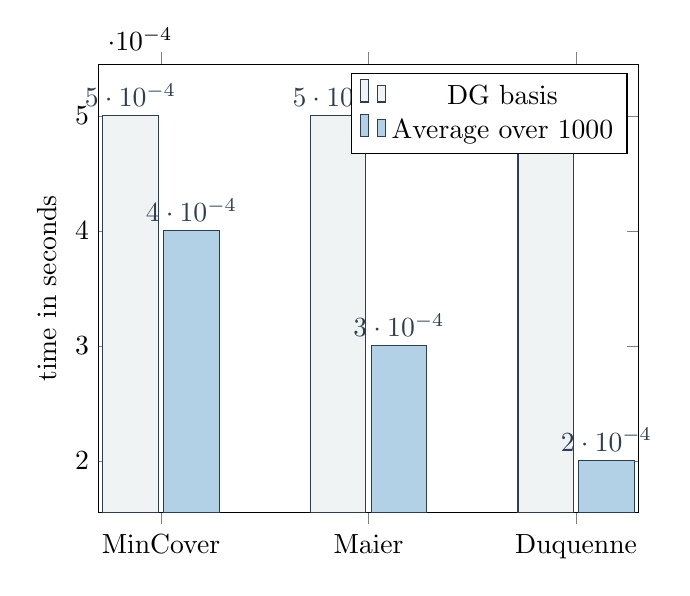
\begin{tikzpicture}
\begin{axis}[
ybar,
bar width=20pt,
enlargelimits=0.15,
ylabel={time in seconds},
symbolic x coords={MinCover, Maier, Duquenne},
xtick=data,
nodes near coords,
nodes near coords align={vertical},
]
\addplot[midnight, fill=clouds!80!white]
	 coordinates {(MinCover, 0.0005) (Maier, 0.0005) (Duquenne, 0.0005)};
\addplot[midnight, fill=belize!30!white] coordinates {(MinCover, 0.0004) (Maier, 0.0003) (Duquenne, 0.0002)};
\legend{DG basis, Average over 1000}
\end{axis}
\end{tikzpicture}
}
\subfloat[Zoo - Min]{
	
	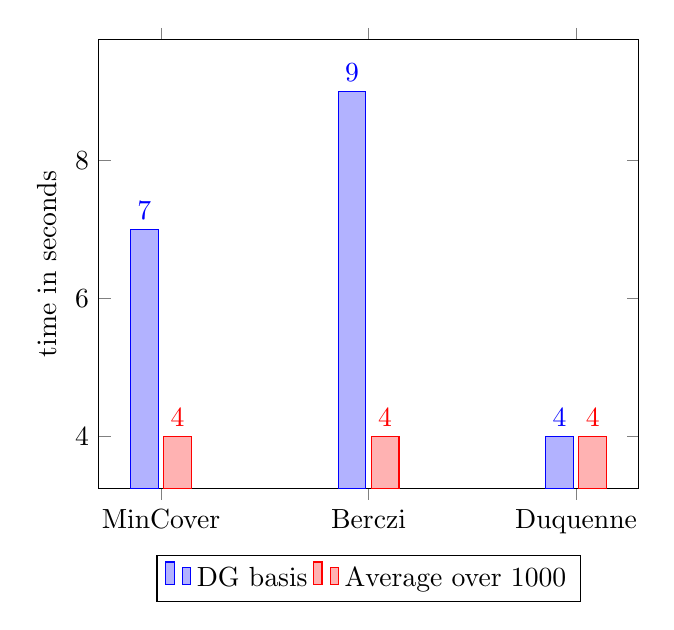
\begin{tikzpicture}
	\begin{axis}[
	ybar,
	enlargelimits=0.15,
	legend style={at={(0.5,-0.15)},
		anchor=north,legend columns=-1},
	ylabel={time in seconds},
	symbolic x coords={MinCover, Berczi, Duquenne},
	xtick=data,
	nodes near coords,
	nodes near coords align={vertical},
	]
	\addplot coordinates {(MinCover, 7) (Berczi,9) (Duquenne,4)};
	\addplot coordinates {(MinCover,4) (Berczi,4) (Duquenne,4)};
	\legend{DG basis, Average over 1000}
	\end{axis}
	\end{tikzpicture}
}
\end{figure}

Each graph corresponds to a dataset. Inside all of them, we have a series
of bar plots per algorithm. In order, one may find the time (in seconds) required for the Duquenne-Guigues basis, the minimum basis we had with the
minimal generators, with proper implications and eventually the average
time we obtained for minimization over 2000 randomly generated bases. For \textsc{DuquenneMinimization} and \textsc{MaierMinimization}, it seems like
our hypothesis holds: on average, minimizing a redundant system is less time consuming than a base being minimum, for fixed $|\Sg|$ and $|\B|$. However,
this does not hold for \textsc{MinCover} for which the worst case is often
the minimum bases with non right-closed implications. Moreover reducing a redundant theory is more expensive on average than minimizing right-closed
bases. Our idea is that right-closed results in fast closure computations, because for each implication the information we may get is maximal. In the
case of non-closed implications, we are likely to need several runs over
$\I$ for this task. Then, depending on the order in which we consider implications in the second loop, the execution time may vary. If all redundant
implications are handled before others, we will spare several operations.
On the contrary, if they are all placed at the end, we will maximize the
cost.

Last, we used our random generation tool to try to trace the evolution of
each algorithms when one parameter is fixed, namely $|\Sg|$. One can observe
the results in figure \ref{fig:random}. We would like to emphasize on the experimental aspect of those results: they act as a hint for further work and not as a ground for hypothesis as previous ones. Observe that in smallest case, \textsc{AFP} is faster than all other algorithms, while in the other one,
results coincide with observed real data. It can be due to random generation only exploring one part of the system space being (for instance) highly redundant. It could also be related to the small size of the dataset we are minimizing here. Whether those observation are to be investigated or not is a matter of further study and experiment. Still, they depict interesting track to
follow in the future on the behaviour of \textsc{AFP} as much as the underlying
structure of our implication systems.

\begin{figure}
	\begin{minipage}{0.4\textwidth}
		\hspace{-3em}
		\subfloat[Average time, $|\Sg| = 100$]{
			\scalebox{0.4}{%% Creator: Matplotlib, PGF backend
%%
%% To include the figure in your LaTeX document, write
%%   \input{<filename>.pgf}
%%
%% Make sure the required packages are loaded in your preamble
%%   \usepackage{pgf}
%%
%% Figures using additional raster images can only be included by \input if
%% they are in the same directory as the main LaTeX file. For loading figures
%% from other directories you can use the `import` package
%%   \usepackage{import}
%% and then include the figures with
%%   \import{<path to file>}{<filename>.pgf}
%%
%% Matplotlib used the following preamble
%%   \usepackage{fontspec}
%%   \setmainfont{DejaVu Serif}
%%   \setsansfont{DejaVu Sans}
%%   \setmonofont{DejaVu Sans Mono}
%%
\begingroup%
\makeatletter%
\begin{pgfpicture}%
\pgfpathrectangle{\pgfpointorigin}{\pgfqpoint{6.400000in}{4.800000in}}%
\pgfusepath{use as bounding box, clip}%
\begin{pgfscope}%
\pgfsetbuttcap%
\pgfsetmiterjoin%
\definecolor{currentfill}{rgb}{1.000000,1.000000,1.000000}%
\pgfsetfillcolor{currentfill}%
\pgfsetlinewidth{0.000000pt}%
\definecolor{currentstroke}{rgb}{1.000000,1.000000,1.000000}%
\pgfsetstrokecolor{currentstroke}%
\pgfsetdash{}{0pt}%
\pgfpathmoveto{\pgfqpoint{0.000000in}{0.000000in}}%
\pgfpathlineto{\pgfqpoint{6.400000in}{0.000000in}}%
\pgfpathlineto{\pgfqpoint{6.400000in}{4.800000in}}%
\pgfpathlineto{\pgfqpoint{0.000000in}{4.800000in}}%
\pgfpathclose%
\pgfusepath{fill}%
\end{pgfscope}%
\begin{pgfscope}%
\pgfsetbuttcap%
\pgfsetmiterjoin%
\definecolor{currentfill}{rgb}{1.000000,1.000000,1.000000}%
\pgfsetfillcolor{currentfill}%
\pgfsetlinewidth{0.000000pt}%
\definecolor{currentstroke}{rgb}{0.000000,0.000000,0.000000}%
\pgfsetstrokecolor{currentstroke}%
\pgfsetstrokeopacity{0.000000}%
\pgfsetdash{}{0pt}%
\pgfpathmoveto{\pgfqpoint{0.800000in}{0.528000in}}%
\pgfpathlineto{\pgfqpoint{5.760000in}{0.528000in}}%
\pgfpathlineto{\pgfqpoint{5.760000in}{4.224000in}}%
\pgfpathlineto{\pgfqpoint{0.800000in}{4.224000in}}%
\pgfpathclose%
\pgfusepath{fill}%
\end{pgfscope}%
\begin{pgfscope}%
\pgfsetbuttcap%
\pgfsetroundjoin%
\definecolor{currentfill}{rgb}{0.000000,0.000000,0.000000}%
\pgfsetfillcolor{currentfill}%
\pgfsetlinewidth{0.803000pt}%
\definecolor{currentstroke}{rgb}{0.000000,0.000000,0.000000}%
\pgfsetstrokecolor{currentstroke}%
\pgfsetdash{}{0pt}%
\pgfsys@defobject{currentmarker}{\pgfqpoint{0.000000in}{-0.048611in}}{\pgfqpoint{0.000000in}{0.000000in}}{%
\pgfpathmoveto{\pgfqpoint{0.000000in}{0.000000in}}%
\pgfpathlineto{\pgfqpoint{0.000000in}{-0.048611in}}%
\pgfusepath{stroke,fill}%
}%
\begin{pgfscope}%
\pgfsys@transformshift{0.974215in}{0.528000in}%
\pgfsys@useobject{currentmarker}{}%
\end{pgfscope}%
\end{pgfscope}%
\begin{pgfscope}%
\pgftext[x=0.974215in,y=0.430778in,,top]{\sffamily\fontsize{10.000000}{12.000000}\selectfont \(\displaystyle 0\)}%
\end{pgfscope}%
\begin{pgfscope}%
\pgfsetbuttcap%
\pgfsetroundjoin%
\definecolor{currentfill}{rgb}{0.000000,0.000000,0.000000}%
\pgfsetfillcolor{currentfill}%
\pgfsetlinewidth{0.803000pt}%
\definecolor{currentstroke}{rgb}{0.000000,0.000000,0.000000}%
\pgfsetstrokecolor{currentstroke}%
\pgfsetdash{}{0pt}%
\pgfsys@defobject{currentmarker}{\pgfqpoint{0.000000in}{-0.048611in}}{\pgfqpoint{0.000000in}{0.000000in}}{%
\pgfpathmoveto{\pgfqpoint{0.000000in}{0.000000in}}%
\pgfpathlineto{\pgfqpoint{0.000000in}{-0.048611in}}%
\pgfusepath{stroke,fill}%
}%
\begin{pgfscope}%
\pgfsys@transformshift{1.486612in}{0.528000in}%
\pgfsys@useobject{currentmarker}{}%
\end{pgfscope}%
\end{pgfscope}%
\begin{pgfscope}%
\pgftext[x=1.486612in,y=0.430778in,,top]{\sffamily\fontsize{10.000000}{12.000000}\selectfont \(\displaystyle 1000\)}%
\end{pgfscope}%
\begin{pgfscope}%
\pgfsetbuttcap%
\pgfsetroundjoin%
\definecolor{currentfill}{rgb}{0.000000,0.000000,0.000000}%
\pgfsetfillcolor{currentfill}%
\pgfsetlinewidth{0.803000pt}%
\definecolor{currentstroke}{rgb}{0.000000,0.000000,0.000000}%
\pgfsetstrokecolor{currentstroke}%
\pgfsetdash{}{0pt}%
\pgfsys@defobject{currentmarker}{\pgfqpoint{0.000000in}{-0.048611in}}{\pgfqpoint{0.000000in}{0.000000in}}{%
\pgfpathmoveto{\pgfqpoint{0.000000in}{0.000000in}}%
\pgfpathlineto{\pgfqpoint{0.000000in}{-0.048611in}}%
\pgfusepath{stroke,fill}%
}%
\begin{pgfscope}%
\pgfsys@transformshift{1.999008in}{0.528000in}%
\pgfsys@useobject{currentmarker}{}%
\end{pgfscope}%
\end{pgfscope}%
\begin{pgfscope}%
\pgftext[x=1.999008in,y=0.430778in,,top]{\sffamily\fontsize{10.000000}{12.000000}\selectfont \(\displaystyle 2000\)}%
\end{pgfscope}%
\begin{pgfscope}%
\pgfsetbuttcap%
\pgfsetroundjoin%
\definecolor{currentfill}{rgb}{0.000000,0.000000,0.000000}%
\pgfsetfillcolor{currentfill}%
\pgfsetlinewidth{0.803000pt}%
\definecolor{currentstroke}{rgb}{0.000000,0.000000,0.000000}%
\pgfsetstrokecolor{currentstroke}%
\pgfsetdash{}{0pt}%
\pgfsys@defobject{currentmarker}{\pgfqpoint{0.000000in}{-0.048611in}}{\pgfqpoint{0.000000in}{0.000000in}}{%
\pgfpathmoveto{\pgfqpoint{0.000000in}{0.000000in}}%
\pgfpathlineto{\pgfqpoint{0.000000in}{-0.048611in}}%
\pgfusepath{stroke,fill}%
}%
\begin{pgfscope}%
\pgfsys@transformshift{2.511405in}{0.528000in}%
\pgfsys@useobject{currentmarker}{}%
\end{pgfscope}%
\end{pgfscope}%
\begin{pgfscope}%
\pgftext[x=2.511405in,y=0.430778in,,top]{\sffamily\fontsize{10.000000}{12.000000}\selectfont \(\displaystyle 3000\)}%
\end{pgfscope}%
\begin{pgfscope}%
\pgfsetbuttcap%
\pgfsetroundjoin%
\definecolor{currentfill}{rgb}{0.000000,0.000000,0.000000}%
\pgfsetfillcolor{currentfill}%
\pgfsetlinewidth{0.803000pt}%
\definecolor{currentstroke}{rgb}{0.000000,0.000000,0.000000}%
\pgfsetstrokecolor{currentstroke}%
\pgfsetdash{}{0pt}%
\pgfsys@defobject{currentmarker}{\pgfqpoint{0.000000in}{-0.048611in}}{\pgfqpoint{0.000000in}{0.000000in}}{%
\pgfpathmoveto{\pgfqpoint{0.000000in}{0.000000in}}%
\pgfpathlineto{\pgfqpoint{0.000000in}{-0.048611in}}%
\pgfusepath{stroke,fill}%
}%
\begin{pgfscope}%
\pgfsys@transformshift{3.023802in}{0.528000in}%
\pgfsys@useobject{currentmarker}{}%
\end{pgfscope}%
\end{pgfscope}%
\begin{pgfscope}%
\pgftext[x=3.023802in,y=0.430778in,,top]{\sffamily\fontsize{10.000000}{12.000000}\selectfont \(\displaystyle 4000\)}%
\end{pgfscope}%
\begin{pgfscope}%
\pgfsetbuttcap%
\pgfsetroundjoin%
\definecolor{currentfill}{rgb}{0.000000,0.000000,0.000000}%
\pgfsetfillcolor{currentfill}%
\pgfsetlinewidth{0.803000pt}%
\definecolor{currentstroke}{rgb}{0.000000,0.000000,0.000000}%
\pgfsetstrokecolor{currentstroke}%
\pgfsetdash{}{0pt}%
\pgfsys@defobject{currentmarker}{\pgfqpoint{0.000000in}{-0.048611in}}{\pgfqpoint{0.000000in}{0.000000in}}{%
\pgfpathmoveto{\pgfqpoint{0.000000in}{0.000000in}}%
\pgfpathlineto{\pgfqpoint{0.000000in}{-0.048611in}}%
\pgfusepath{stroke,fill}%
}%
\begin{pgfscope}%
\pgfsys@transformshift{3.536198in}{0.528000in}%
\pgfsys@useobject{currentmarker}{}%
\end{pgfscope}%
\end{pgfscope}%
\begin{pgfscope}%
\pgftext[x=3.536198in,y=0.430778in,,top]{\sffamily\fontsize{10.000000}{12.000000}\selectfont \(\displaystyle 5000\)}%
\end{pgfscope}%
\begin{pgfscope}%
\pgfsetbuttcap%
\pgfsetroundjoin%
\definecolor{currentfill}{rgb}{0.000000,0.000000,0.000000}%
\pgfsetfillcolor{currentfill}%
\pgfsetlinewidth{0.803000pt}%
\definecolor{currentstroke}{rgb}{0.000000,0.000000,0.000000}%
\pgfsetstrokecolor{currentstroke}%
\pgfsetdash{}{0pt}%
\pgfsys@defobject{currentmarker}{\pgfqpoint{0.000000in}{-0.048611in}}{\pgfqpoint{0.000000in}{0.000000in}}{%
\pgfpathmoveto{\pgfqpoint{0.000000in}{0.000000in}}%
\pgfpathlineto{\pgfqpoint{0.000000in}{-0.048611in}}%
\pgfusepath{stroke,fill}%
}%
\begin{pgfscope}%
\pgfsys@transformshift{4.048595in}{0.528000in}%
\pgfsys@useobject{currentmarker}{}%
\end{pgfscope}%
\end{pgfscope}%
\begin{pgfscope}%
\pgftext[x=4.048595in,y=0.430778in,,top]{\sffamily\fontsize{10.000000}{12.000000}\selectfont \(\displaystyle 6000\)}%
\end{pgfscope}%
\begin{pgfscope}%
\pgfsetbuttcap%
\pgfsetroundjoin%
\definecolor{currentfill}{rgb}{0.000000,0.000000,0.000000}%
\pgfsetfillcolor{currentfill}%
\pgfsetlinewidth{0.803000pt}%
\definecolor{currentstroke}{rgb}{0.000000,0.000000,0.000000}%
\pgfsetstrokecolor{currentstroke}%
\pgfsetdash{}{0pt}%
\pgfsys@defobject{currentmarker}{\pgfqpoint{0.000000in}{-0.048611in}}{\pgfqpoint{0.000000in}{0.000000in}}{%
\pgfpathmoveto{\pgfqpoint{0.000000in}{0.000000in}}%
\pgfpathlineto{\pgfqpoint{0.000000in}{-0.048611in}}%
\pgfusepath{stroke,fill}%
}%
\begin{pgfscope}%
\pgfsys@transformshift{4.560992in}{0.528000in}%
\pgfsys@useobject{currentmarker}{}%
\end{pgfscope}%
\end{pgfscope}%
\begin{pgfscope}%
\pgftext[x=4.560992in,y=0.430778in,,top]{\sffamily\fontsize{10.000000}{12.000000}\selectfont \(\displaystyle 7000\)}%
\end{pgfscope}%
\begin{pgfscope}%
\pgfsetbuttcap%
\pgfsetroundjoin%
\definecolor{currentfill}{rgb}{0.000000,0.000000,0.000000}%
\pgfsetfillcolor{currentfill}%
\pgfsetlinewidth{0.803000pt}%
\definecolor{currentstroke}{rgb}{0.000000,0.000000,0.000000}%
\pgfsetstrokecolor{currentstroke}%
\pgfsetdash{}{0pt}%
\pgfsys@defobject{currentmarker}{\pgfqpoint{0.000000in}{-0.048611in}}{\pgfqpoint{0.000000in}{0.000000in}}{%
\pgfpathmoveto{\pgfqpoint{0.000000in}{0.000000in}}%
\pgfpathlineto{\pgfqpoint{0.000000in}{-0.048611in}}%
\pgfusepath{stroke,fill}%
}%
\begin{pgfscope}%
\pgfsys@transformshift{5.073388in}{0.528000in}%
\pgfsys@useobject{currentmarker}{}%
\end{pgfscope}%
\end{pgfscope}%
\begin{pgfscope}%
\pgftext[x=5.073388in,y=0.430778in,,top]{\sffamily\fontsize{10.000000}{12.000000}\selectfont \(\displaystyle 8000\)}%
\end{pgfscope}%
\begin{pgfscope}%
\pgfsetbuttcap%
\pgfsetroundjoin%
\definecolor{currentfill}{rgb}{0.000000,0.000000,0.000000}%
\pgfsetfillcolor{currentfill}%
\pgfsetlinewidth{0.803000pt}%
\definecolor{currentstroke}{rgb}{0.000000,0.000000,0.000000}%
\pgfsetstrokecolor{currentstroke}%
\pgfsetdash{}{0pt}%
\pgfsys@defobject{currentmarker}{\pgfqpoint{0.000000in}{-0.048611in}}{\pgfqpoint{0.000000in}{0.000000in}}{%
\pgfpathmoveto{\pgfqpoint{0.000000in}{0.000000in}}%
\pgfpathlineto{\pgfqpoint{0.000000in}{-0.048611in}}%
\pgfusepath{stroke,fill}%
}%
\begin{pgfscope}%
\pgfsys@transformshift{5.585785in}{0.528000in}%
\pgfsys@useobject{currentmarker}{}%
\end{pgfscope}%
\end{pgfscope}%
\begin{pgfscope}%
\pgftext[x=5.585785in,y=0.430778in,,top]{\sffamily\fontsize{10.000000}{12.000000}\selectfont \(\displaystyle 9000\)}%
\end{pgfscope}%
\begin{pgfscope}%
\pgftext[x=3.280000in,y=0.240809in,,top]{\sffamily\fontsize{14.000000}{16.800000}\selectfont \(\displaystyle |\mathcal{B}|\)}%
\end{pgfscope}%
\begin{pgfscope}%
\pgfsetbuttcap%
\pgfsetroundjoin%
\definecolor{currentfill}{rgb}{0.000000,0.000000,0.000000}%
\pgfsetfillcolor{currentfill}%
\pgfsetlinewidth{0.803000pt}%
\definecolor{currentstroke}{rgb}{0.000000,0.000000,0.000000}%
\pgfsetstrokecolor{currentstroke}%
\pgfsetdash{}{0pt}%
\pgfsys@defobject{currentmarker}{\pgfqpoint{-0.048611in}{0.000000in}}{\pgfqpoint{0.000000in}{0.000000in}}{%
\pgfpathmoveto{\pgfqpoint{0.000000in}{0.000000in}}%
\pgfpathlineto{\pgfqpoint{-0.048611in}{0.000000in}}%
\pgfusepath{stroke,fill}%
}%
\begin{pgfscope}%
\pgfsys@transformshift{0.800000in}{0.695391in}%
\pgfsys@useobject{currentmarker}{}%
\end{pgfscope}%
\end{pgfscope}%
\begin{pgfscope}%
\pgftext[x=0.525308in,y=0.642629in,left,base]{\sffamily\fontsize{10.000000}{12.000000}\selectfont \(\displaystyle 0.0\)}%
\end{pgfscope}%
\begin{pgfscope}%
\pgfsetbuttcap%
\pgfsetroundjoin%
\definecolor{currentfill}{rgb}{0.000000,0.000000,0.000000}%
\pgfsetfillcolor{currentfill}%
\pgfsetlinewidth{0.803000pt}%
\definecolor{currentstroke}{rgb}{0.000000,0.000000,0.000000}%
\pgfsetstrokecolor{currentstroke}%
\pgfsetdash{}{0pt}%
\pgfsys@defobject{currentmarker}{\pgfqpoint{-0.048611in}{0.000000in}}{\pgfqpoint{0.000000in}{0.000000in}}{%
\pgfpathmoveto{\pgfqpoint{0.000000in}{0.000000in}}%
\pgfpathlineto{\pgfqpoint{-0.048611in}{0.000000in}}%
\pgfusepath{stroke,fill}%
}%
\begin{pgfscope}%
\pgfsys@transformshift{0.800000in}{1.345154in}%
\pgfsys@useobject{currentmarker}{}%
\end{pgfscope}%
\end{pgfscope}%
\begin{pgfscope}%
\pgftext[x=0.525308in,y=1.292393in,left,base]{\sffamily\fontsize{10.000000}{12.000000}\selectfont \(\displaystyle 0.2\)}%
\end{pgfscope}%
\begin{pgfscope}%
\pgfsetbuttcap%
\pgfsetroundjoin%
\definecolor{currentfill}{rgb}{0.000000,0.000000,0.000000}%
\pgfsetfillcolor{currentfill}%
\pgfsetlinewidth{0.803000pt}%
\definecolor{currentstroke}{rgb}{0.000000,0.000000,0.000000}%
\pgfsetstrokecolor{currentstroke}%
\pgfsetdash{}{0pt}%
\pgfsys@defobject{currentmarker}{\pgfqpoint{-0.048611in}{0.000000in}}{\pgfqpoint{0.000000in}{0.000000in}}{%
\pgfpathmoveto{\pgfqpoint{0.000000in}{0.000000in}}%
\pgfpathlineto{\pgfqpoint{-0.048611in}{0.000000in}}%
\pgfusepath{stroke,fill}%
}%
\begin{pgfscope}%
\pgfsys@transformshift{0.800000in}{1.994918in}%
\pgfsys@useobject{currentmarker}{}%
\end{pgfscope}%
\end{pgfscope}%
\begin{pgfscope}%
\pgftext[x=0.525308in,y=1.942156in,left,base]{\sffamily\fontsize{10.000000}{12.000000}\selectfont \(\displaystyle 0.4\)}%
\end{pgfscope}%
\begin{pgfscope}%
\pgfsetbuttcap%
\pgfsetroundjoin%
\definecolor{currentfill}{rgb}{0.000000,0.000000,0.000000}%
\pgfsetfillcolor{currentfill}%
\pgfsetlinewidth{0.803000pt}%
\definecolor{currentstroke}{rgb}{0.000000,0.000000,0.000000}%
\pgfsetstrokecolor{currentstroke}%
\pgfsetdash{}{0pt}%
\pgfsys@defobject{currentmarker}{\pgfqpoint{-0.048611in}{0.000000in}}{\pgfqpoint{0.000000in}{0.000000in}}{%
\pgfpathmoveto{\pgfqpoint{0.000000in}{0.000000in}}%
\pgfpathlineto{\pgfqpoint{-0.048611in}{0.000000in}}%
\pgfusepath{stroke,fill}%
}%
\begin{pgfscope}%
\pgfsys@transformshift{0.800000in}{2.644681in}%
\pgfsys@useobject{currentmarker}{}%
\end{pgfscope}%
\end{pgfscope}%
\begin{pgfscope}%
\pgftext[x=0.525308in,y=2.591920in,left,base]{\sffamily\fontsize{10.000000}{12.000000}\selectfont \(\displaystyle 0.6\)}%
\end{pgfscope}%
\begin{pgfscope}%
\pgfsetbuttcap%
\pgfsetroundjoin%
\definecolor{currentfill}{rgb}{0.000000,0.000000,0.000000}%
\pgfsetfillcolor{currentfill}%
\pgfsetlinewidth{0.803000pt}%
\definecolor{currentstroke}{rgb}{0.000000,0.000000,0.000000}%
\pgfsetstrokecolor{currentstroke}%
\pgfsetdash{}{0pt}%
\pgfsys@defobject{currentmarker}{\pgfqpoint{-0.048611in}{0.000000in}}{\pgfqpoint{0.000000in}{0.000000in}}{%
\pgfpathmoveto{\pgfqpoint{0.000000in}{0.000000in}}%
\pgfpathlineto{\pgfqpoint{-0.048611in}{0.000000in}}%
\pgfusepath{stroke,fill}%
}%
\begin{pgfscope}%
\pgfsys@transformshift{0.800000in}{3.294445in}%
\pgfsys@useobject{currentmarker}{}%
\end{pgfscope}%
\end{pgfscope}%
\begin{pgfscope}%
\pgftext[x=0.525308in,y=3.241683in,left,base]{\sffamily\fontsize{10.000000}{12.000000}\selectfont \(\displaystyle 0.8\)}%
\end{pgfscope}%
\begin{pgfscope}%
\pgfsetbuttcap%
\pgfsetroundjoin%
\definecolor{currentfill}{rgb}{0.000000,0.000000,0.000000}%
\pgfsetfillcolor{currentfill}%
\pgfsetlinewidth{0.803000pt}%
\definecolor{currentstroke}{rgb}{0.000000,0.000000,0.000000}%
\pgfsetstrokecolor{currentstroke}%
\pgfsetdash{}{0pt}%
\pgfsys@defobject{currentmarker}{\pgfqpoint{-0.048611in}{0.000000in}}{\pgfqpoint{0.000000in}{0.000000in}}{%
\pgfpathmoveto{\pgfqpoint{0.000000in}{0.000000in}}%
\pgfpathlineto{\pgfqpoint{-0.048611in}{0.000000in}}%
\pgfusepath{stroke,fill}%
}%
\begin{pgfscope}%
\pgfsys@transformshift{0.800000in}{3.944208in}%
\pgfsys@useobject{currentmarker}{}%
\end{pgfscope}%
\end{pgfscope}%
\begin{pgfscope}%
\pgftext[x=0.525308in,y=3.891447in,left,base]{\sffamily\fontsize{10.000000}{12.000000}\selectfont \(\displaystyle 1.0\)}%
\end{pgfscope}%
\begin{pgfscope}%
\pgftext[x=0.469752in,y=2.376000in,,bottom,rotate=90.000000]{\sffamily\fontsize{14.000000}{16.800000}\selectfont seconds}%
\end{pgfscope}%
\begin{pgfscope}%
\pgfpathrectangle{\pgfqpoint{0.800000in}{0.528000in}}{\pgfqpoint{4.960000in}{3.696000in}}%
\pgfusepath{clip}%
\pgfsetrectcap%
\pgfsetroundjoin%
\pgfsetlinewidth{1.505625pt}%
\definecolor{currentstroke}{rgb}{0.172549,0.243137,0.313725}%
\pgfsetstrokecolor{currentstroke}%
\pgfsetdash{}{0pt}%
\pgfpathmoveto{\pgfqpoint{1.025455in}{0.700467in}}%
\pgfpathlineto{\pgfqpoint{1.076694in}{0.707269in}}%
\pgfpathlineto{\pgfqpoint{1.127934in}{0.711736in}}%
\pgfpathlineto{\pgfqpoint{1.179174in}{0.719859in}}%
\pgfpathlineto{\pgfqpoint{1.230413in}{0.724224in}}%
\pgfpathlineto{\pgfqpoint{1.281653in}{0.728590in}}%
\pgfpathlineto{\pgfqpoint{1.332893in}{0.732244in}}%
\pgfpathlineto{\pgfqpoint{1.384132in}{0.740773in}}%
\pgfpathlineto{\pgfqpoint{1.435372in}{0.744224in}}%
\pgfpathlineto{\pgfqpoint{1.486612in}{0.753362in}}%
\pgfpathlineto{\pgfqpoint{1.537851in}{0.756915in}}%
\pgfpathlineto{\pgfqpoint{1.589091in}{0.766154in}}%
\pgfpathlineto{\pgfqpoint{1.640331in}{0.770520in}}%
\pgfpathlineto{\pgfqpoint{1.691570in}{0.772753in}}%
\pgfpathlineto{\pgfqpoint{1.742810in}{0.772753in}}%
\pgfpathlineto{\pgfqpoint{1.794050in}{0.784835in}}%
\pgfpathlineto{\pgfqpoint{1.845289in}{0.791028in}}%
\pgfpathlineto{\pgfqpoint{1.896529in}{0.791028in}}%
\pgfpathlineto{\pgfqpoint{1.947769in}{0.794987in}}%
\pgfpathlineto{\pgfqpoint{1.999008in}{0.801485in}}%
\pgfpathlineto{\pgfqpoint{2.050248in}{0.806764in}}%
\pgfpathlineto{\pgfqpoint{2.101488in}{0.839151in}}%
\pgfpathlineto{\pgfqpoint{2.152727in}{0.856918in}}%
\pgfpathlineto{\pgfqpoint{2.203967in}{0.871132in}}%
\pgfpathlineto{\pgfqpoint{2.255207in}{0.884736in}}%
\pgfpathlineto{\pgfqpoint{2.306446in}{0.871639in}}%
\pgfpathlineto{\pgfqpoint{2.357686in}{0.834989in}}%
\pgfpathlineto{\pgfqpoint{2.408926in}{0.825851in}}%
\pgfpathlineto{\pgfqpoint{2.460165in}{0.838034in}}%
\pgfpathlineto{\pgfqpoint{2.511405in}{0.844430in}}%
\pgfpathlineto{\pgfqpoint{2.562645in}{0.850319in}}%
\pgfpathlineto{\pgfqpoint{2.613884in}{0.857527in}}%
\pgfpathlineto{\pgfqpoint{2.665124in}{0.857629in}}%
\pgfpathlineto{\pgfqpoint{2.716364in}{0.863619in}}%
\pgfpathlineto{\pgfqpoint{2.767603in}{0.866055in}}%
\pgfpathlineto{\pgfqpoint{2.818843in}{0.880370in}}%
\pgfpathlineto{\pgfqpoint{2.870083in}{0.869710in}}%
\pgfpathlineto{\pgfqpoint{2.921322in}{0.871842in}}%
\pgfpathlineto{\pgfqpoint{2.972562in}{0.894990in}}%
\pgfpathlineto{\pgfqpoint{3.023802in}{0.930930in}}%
\pgfpathlineto{\pgfqpoint{3.075041in}{0.940169in}}%
\pgfpathlineto{\pgfqpoint{3.126281in}{0.958850in}}%
\pgfpathlineto{\pgfqpoint{3.177521in}{0.949916in}}%
\pgfpathlineto{\pgfqpoint{3.228760in}{0.928493in}}%
\pgfpathlineto{\pgfqpoint{3.280000in}{0.922504in}}%
\pgfpathlineto{\pgfqpoint{3.331240in}{0.929915in}}%
\pgfpathlineto{\pgfqpoint{3.382479in}{0.924128in}}%
\pgfpathlineto{\pgfqpoint{3.433719in}{0.911437in}}%
\pgfpathlineto{\pgfqpoint{3.484959in}{0.916006in}}%
\pgfpathlineto{\pgfqpoint{3.536198in}{0.915701in}}%
\pgfpathlineto{\pgfqpoint{3.587438in}{0.913772in}}%
\pgfpathlineto{\pgfqpoint{3.638678in}{0.923823in}}%
\pgfpathlineto{\pgfqpoint{3.689917in}{0.933367in}}%
\pgfpathlineto{\pgfqpoint{3.741157in}{0.940778in}}%
\pgfpathlineto{\pgfqpoint{3.792397in}{0.931844in}}%
\pgfpathlineto{\pgfqpoint{3.843636in}{0.943316in}}%
\pgfpathlineto{\pgfqpoint{3.894876in}{0.944027in}}%
\pgfpathlineto{\pgfqpoint{3.946116in}{0.942707in}}%
\pgfpathlineto{\pgfqpoint{3.997355in}{0.967175in}}%
\pgfpathlineto{\pgfqpoint{4.048595in}{1.003927in}}%
\pgfpathlineto{\pgfqpoint{4.099835in}{1.005247in}}%
\pgfpathlineto{\pgfqpoint{4.151074in}{0.990322in}}%
\pgfpathlineto{\pgfqpoint{4.202314in}{0.985246in}}%
\pgfpathlineto{\pgfqpoint{4.253554in}{0.970424in}}%
\pgfpathlineto{\pgfqpoint{4.304793in}{0.980272in}}%
\pgfpathlineto{\pgfqpoint{4.356033in}{1.036010in}}%
\pgfpathlineto{\pgfqpoint{4.407273in}{1.013775in}}%
\pgfpathlineto{\pgfqpoint{4.458512in}{1.023015in}}%
\pgfpathlineto{\pgfqpoint{4.509752in}{1.025451in}}%
\pgfpathlineto{\pgfqpoint{4.560992in}{1.054385in}}%
\pgfpathlineto{\pgfqpoint{4.612231in}{1.055909in}}%
\pgfpathlineto{\pgfqpoint{4.663471in}{1.019359in}}%
\pgfpathlineto{\pgfqpoint{4.714711in}{1.004333in}}%
\pgfpathlineto{\pgfqpoint{4.765950in}{1.016719in}}%
\pgfpathlineto{\pgfqpoint{4.817190in}{1.032150in}}%
\pgfpathlineto{\pgfqpoint{4.868430in}{1.021796in}}%
\pgfpathlineto{\pgfqpoint{4.919669in}{1.079463in}}%
\pgfpathlineto{\pgfqpoint{4.970909in}{1.064538in}}%
\pgfpathlineto{\pgfqpoint{5.022149in}{1.102611in}}%
\pgfpathlineto{\pgfqpoint{5.073388in}{1.090629in}}%
\pgfpathlineto{\pgfqpoint{5.124628in}{1.063521in}}%
\pgfpathlineto{\pgfqpoint{5.175868in}{1.093982in}}%
\pgfpathlineto{\pgfqpoint{5.227107in}{1.115606in}}%
\pgfpathlineto{\pgfqpoint{5.278347in}{1.098855in}}%
\pgfpathlineto{\pgfqpoint{5.329587in}{1.070223in}}%
\pgfpathlineto{\pgfqpoint{5.380826in}{1.068498in}}%
\pgfpathlineto{\pgfqpoint{5.432066in}{1.077939in}}%
\pgfpathlineto{\pgfqpoint{5.483306in}{1.084437in}}%
\pgfpathlineto{\pgfqpoint{5.534545in}{1.147181in}}%
\pgfusepath{stroke}%
\end{pgfscope}%
\begin{pgfscope}%
\pgfpathrectangle{\pgfqpoint{0.800000in}{0.528000in}}{\pgfqpoint{4.960000in}{3.696000in}}%
\pgfusepath{clip}%
\pgfsetrectcap%
\pgfsetroundjoin%
\pgfsetlinewidth{1.505625pt}%
\definecolor{currentstroke}{rgb}{0.160784,0.501961,0.725490}%
\pgfsetstrokecolor{currentstroke}%
\pgfsetdash{}{0pt}%
\pgfpathmoveto{\pgfqpoint{1.025455in}{0.696203in}}%
\pgfpathlineto{\pgfqpoint{1.076694in}{0.697523in}}%
\pgfpathlineto{\pgfqpoint{1.127934in}{0.700061in}}%
\pgfpathlineto{\pgfqpoint{1.179174in}{0.702396in}}%
\pgfpathlineto{\pgfqpoint{1.230413in}{0.706762in}}%
\pgfpathlineto{\pgfqpoint{1.281653in}{0.709097in}}%
\pgfpathlineto{\pgfqpoint{1.332893in}{0.712853in}}%
\pgfpathlineto{\pgfqpoint{1.384132in}{0.721381in}}%
\pgfpathlineto{\pgfqpoint{1.435372in}{0.725950in}}%
\pgfpathlineto{\pgfqpoint{1.486612in}{0.735291in}}%
\pgfpathlineto{\pgfqpoint{1.537851in}{0.738945in}}%
\pgfpathlineto{\pgfqpoint{1.589091in}{0.753463in}}%
\pgfpathlineto{\pgfqpoint{1.640331in}{0.766662in}}%
\pgfpathlineto{\pgfqpoint{1.691570in}{0.774886in}}%
\pgfpathlineto{\pgfqpoint{1.742810in}{0.781992in}}%
\pgfpathlineto{\pgfqpoint{1.794050in}{0.795799in}}%
\pgfpathlineto{\pgfqpoint{1.845289in}{0.814176in}}%
\pgfpathlineto{\pgfqpoint{1.896529in}{0.827780in}}%
\pgfpathlineto{\pgfqpoint{1.947769in}{0.836004in}}%
\pgfpathlineto{\pgfqpoint{1.999008in}{0.845039in}}%
\pgfpathlineto{\pgfqpoint{2.050248in}{0.882502in}}%
\pgfpathlineto{\pgfqpoint{2.101488in}{0.921184in}}%
\pgfpathlineto{\pgfqpoint{2.152727in}{0.967987in}}%
\pgfpathlineto{\pgfqpoint{2.203967in}{1.006160in}}%
\pgfpathlineto{\pgfqpoint{2.255207in}{1.040984in}}%
\pgfpathlineto{\pgfqpoint{2.306446in}{1.036617in}}%
\pgfpathlineto{\pgfqpoint{2.357686in}{0.979662in}}%
\pgfpathlineto{\pgfqpoint{2.408926in}{0.978952in}}%
\pgfpathlineto{\pgfqpoint{2.460165in}{1.014283in}}%
\pgfpathlineto{\pgfqpoint{2.511405in}{1.040678in}}%
\pgfpathlineto{\pgfqpoint{2.562645in}{1.063826in}}%
\pgfpathlineto{\pgfqpoint{2.613884in}{1.076315in}}%
\pgfpathlineto{\pgfqpoint{2.665124in}{1.100986in}}%
\pgfpathlineto{\pgfqpoint{2.716364in}{1.137941in}}%
\pgfpathlineto{\pgfqpoint{2.767603in}{1.170024in}}%
\pgfpathlineto{\pgfqpoint{2.818843in}{1.215608in}}%
\pgfpathlineto{\pgfqpoint{2.870083in}{1.188399in}}%
\pgfpathlineto{\pgfqpoint{2.921322in}{1.225049in}}%
\pgfpathlineto{\pgfqpoint{2.972562in}{1.287995in}}%
\pgfpathlineto{\pgfqpoint{3.023802in}{1.419676in}}%
\pgfpathlineto{\pgfqpoint{3.075041in}{1.470438in}}%
\pgfpathlineto{\pgfqpoint{3.126281in}{1.561707in}}%
\pgfpathlineto{\pgfqpoint{3.177521in}{1.523534in}}%
\pgfpathlineto{\pgfqpoint{3.228760in}{1.500386in}}%
\pgfpathlineto{\pgfqpoint{3.280000in}{1.527595in}}%
\pgfpathlineto{\pgfqpoint{3.331240in}{1.545262in}}%
\pgfpathlineto{\pgfqpoint{3.382479in}{1.572672in}}%
\pgfpathlineto{\pgfqpoint{3.433719in}{1.521302in}}%
\pgfpathlineto{\pgfqpoint{3.484959in}{1.564550in}}%
\pgfpathlineto{\pgfqpoint{3.536198in}{1.569729in}}%
\pgfpathlineto{\pgfqpoint{3.587438in}{1.603029in}}%
\pgfpathlineto{\pgfqpoint{3.638678in}{1.648207in}}%
\pgfpathlineto{\pgfqpoint{3.689917in}{1.713690in}}%
\pgfpathlineto{\pgfqpoint{3.741157in}{1.770343in}}%
\pgfpathlineto{\pgfqpoint{3.792397in}{1.736026in}}%
\pgfpathlineto{\pgfqpoint{3.843636in}{1.843341in}}%
\pgfpathlineto{\pgfqpoint{3.894876in}{1.795928in}}%
\pgfpathlineto{\pgfqpoint{3.946116in}{1.822831in}}%
\pgfpathlineto{\pgfqpoint{3.997355in}{2.059488in}}%
\pgfpathlineto{\pgfqpoint{4.048595in}{2.172180in}}%
\pgfpathlineto{\pgfqpoint{4.099835in}{2.240710in}}%
\pgfpathlineto{\pgfqpoint{4.151074in}{2.168525in}}%
\pgfpathlineto{\pgfqpoint{4.202314in}{2.222030in}}%
\pgfpathlineto{\pgfqpoint{4.253554in}{2.150656in}}%
\pgfpathlineto{\pgfqpoint{4.304793in}{2.215737in}}%
\pgfpathlineto{\pgfqpoint{4.356033in}{2.495742in}}%
\pgfpathlineto{\pgfqpoint{4.407273in}{2.504777in}}%
\pgfpathlineto{\pgfqpoint{4.458512in}{2.523357in}}%
\pgfpathlineto{\pgfqpoint{4.509752in}{2.572902in}}%
\pgfpathlineto{\pgfqpoint{4.560992in}{2.728338in}}%
\pgfpathlineto{\pgfqpoint{4.612231in}{2.810878in}}%
\pgfpathlineto{\pgfqpoint{4.663471in}{2.636865in}}%
\pgfpathlineto{\pgfqpoint{4.714711in}{2.494830in}}%
\pgfpathlineto{\pgfqpoint{4.765950in}{2.643057in}}%
\pgfpathlineto{\pgfqpoint{4.817190in}{2.791489in}}%
\pgfpathlineto{\pgfqpoint{4.868430in}{2.739508in}}%
\pgfpathlineto{\pgfqpoint{4.919669in}{3.097891in}}%
\pgfpathlineto{\pgfqpoint{4.970909in}{2.980528in}}%
\pgfpathlineto{\pgfqpoint{5.022149in}{3.234036in}}%
\pgfpathlineto{\pgfqpoint{5.073388in}{3.247743in}}%
\pgfpathlineto{\pgfqpoint{5.124628in}{3.038701in}}%
\pgfpathlineto{\pgfqpoint{5.175868in}{3.408153in}}%
\pgfpathlineto{\pgfqpoint{5.227107in}{3.511203in}}%
\pgfpathlineto{\pgfqpoint{5.278347in}{3.450489in}}%
\pgfpathlineto{\pgfqpoint{5.329587in}{3.341146in}}%
\pgfpathlineto{\pgfqpoint{5.380826in}{3.335968in}}%
\pgfpathlineto{\pgfqpoint{5.432066in}{3.444602in}}%
\pgfpathlineto{\pgfqpoint{5.483306in}{3.444196in}}%
\pgfpathlineto{\pgfqpoint{5.534545in}{4.056000in}}%
\pgfusepath{stroke}%
\end{pgfscope}%
\begin{pgfscope}%
\pgfpathrectangle{\pgfqpoint{0.800000in}{0.528000in}}{\pgfqpoint{4.960000in}{3.696000in}}%
\pgfusepath{clip}%
\pgfsetrectcap%
\pgfsetroundjoin%
\pgfsetlinewidth{1.505625pt}%
\definecolor{currentstroke}{rgb}{0.905882,0.298039,0.235294}%
\pgfsetstrokecolor{currentstroke}%
\pgfsetdash{}{0pt}%
\pgfpathmoveto{\pgfqpoint{1.025455in}{0.697624in}}%
\pgfpathlineto{\pgfqpoint{1.076694in}{0.701584in}}%
\pgfpathlineto{\pgfqpoint{1.127934in}{0.704122in}}%
\pgfpathlineto{\pgfqpoint{1.179174in}{0.711736in}}%
\pgfpathlineto{\pgfqpoint{1.230413in}{0.711330in}}%
\pgfpathlineto{\pgfqpoint{1.281653in}{0.713462in}}%
\pgfpathlineto{\pgfqpoint{1.332893in}{0.717625in}}%
\pgfpathlineto{\pgfqpoint{1.384132in}{0.721991in}}%
\pgfpathlineto{\pgfqpoint{1.435372in}{0.725645in}}%
\pgfpathlineto{\pgfqpoint{1.486612in}{0.733361in}}%
\pgfpathlineto{\pgfqpoint{1.537851in}{0.737219in}}%
\pgfpathlineto{\pgfqpoint{1.589091in}{0.745849in}}%
\pgfpathlineto{\pgfqpoint{1.640331in}{0.756103in}}%
\pgfpathlineto{\pgfqpoint{1.691570in}{0.760063in}}%
\pgfpathlineto{\pgfqpoint{1.742810in}{0.766154in}}%
\pgfpathlineto{\pgfqpoint{1.794050in}{0.776916in}}%
\pgfpathlineto{\pgfqpoint{1.845289in}{0.786053in}}%
\pgfpathlineto{\pgfqpoint{1.896529in}{0.797322in}}%
\pgfpathlineto{\pgfqpoint{1.947769in}{0.803414in}}%
\pgfpathlineto{\pgfqpoint{1.999008in}{0.811130in}}%
\pgfpathlineto{\pgfqpoint{2.050248in}{0.838136in}}%
\pgfpathlineto{\pgfqpoint{2.101488in}{0.869507in}}%
\pgfpathlineto{\pgfqpoint{2.152727in}{0.896513in}}%
\pgfpathlineto{\pgfqpoint{2.203967in}{0.926463in}}%
\pgfpathlineto{\pgfqpoint{2.255207in}{0.953164in}}%
\pgfpathlineto{\pgfqpoint{2.306446in}{0.943824in}}%
\pgfpathlineto{\pgfqpoint{2.357686in}{0.905346in}}%
\pgfpathlineto{\pgfqpoint{2.408926in}{0.904533in}}%
\pgfpathlineto{\pgfqpoint{2.460165in}{0.928798in}}%
\pgfpathlineto{\pgfqpoint{2.511405in}{0.943113in}}%
\pgfpathlineto{\pgfqpoint{2.562645in}{0.962098in}}%
\pgfpathlineto{\pgfqpoint{2.613884in}{0.973165in}}%
\pgfpathlineto{\pgfqpoint{2.665124in}{0.985246in}}%
\pgfpathlineto{\pgfqpoint{2.716364in}{1.010323in}}%
\pgfpathlineto{\pgfqpoint{2.767603in}{1.032962in}}%
\pgfpathlineto{\pgfqpoint{2.818843in}{1.063625in}}%
\pgfpathlineto{\pgfqpoint{2.870083in}{1.050630in}}%
\pgfpathlineto{\pgfqpoint{2.921322in}{1.070425in}}%
\pgfpathlineto{\pgfqpoint{2.972562in}{1.114082in}}%
\pgfpathlineto{\pgfqpoint{3.023802in}{1.211342in}}%
\pgfpathlineto{\pgfqpoint{3.075041in}{1.234695in}}%
\pgfpathlineto{\pgfqpoint{3.126281in}{1.302514in}}%
\pgfpathlineto{\pgfqpoint{3.177521in}{1.289824in}}%
\pgfpathlineto{\pgfqpoint{3.228760in}{1.269012in}}%
\pgfpathlineto{\pgfqpoint{3.280000in}{1.282816in}}%
\pgfpathlineto{\pgfqpoint{3.331240in}{1.289314in}}%
\pgfpathlineto{\pgfqpoint{3.382479in}{1.307488in}}%
\pgfpathlineto{\pgfqpoint{3.433719in}{1.270532in}}%
\pgfpathlineto{\pgfqpoint{3.484959in}{1.303427in}}%
\pgfpathlineto{\pgfqpoint{3.536198in}{1.305863in}}%
\pgfpathlineto{\pgfqpoint{3.587438in}{1.331854in}}%
\pgfpathlineto{\pgfqpoint{3.638678in}{1.355307in}}%
\pgfpathlineto{\pgfqpoint{3.689917in}{1.405056in}}%
\pgfpathlineto{\pgfqpoint{3.741157in}{1.440588in}}%
\pgfpathlineto{\pgfqpoint{3.792397in}{1.415309in}}%
\pgfpathlineto{\pgfqpoint{3.843636in}{1.493687in}}%
\pgfpathlineto{\pgfqpoint{3.894876in}{1.450741in}}%
\pgfpathlineto{\pgfqpoint{3.946116in}{1.475107in}}%
\pgfpathlineto{\pgfqpoint{3.997355in}{1.635923in}}%
\pgfpathlineto{\pgfqpoint{4.048595in}{1.707602in}}%
\pgfpathlineto{\pgfqpoint{4.099835in}{1.748719in}}%
\pgfpathlineto{\pgfqpoint{4.151074in}{1.706585in}}%
\pgfpathlineto{\pgfqpoint{4.202314in}{1.736536in}}%
\pgfpathlineto{\pgfqpoint{4.253554in}{1.699275in}}%
\pgfpathlineto{\pgfqpoint{4.304793in}{1.735012in}}%
\pgfpathlineto{\pgfqpoint{4.356033in}{1.931771in}}%
\pgfpathlineto{\pgfqpoint{4.407273in}{1.916540in}}%
\pgfpathlineto{\pgfqpoint{4.458512in}{1.951465in}}%
\pgfpathlineto{\pgfqpoint{4.509752in}{1.976442in}}%
\pgfpathlineto{\pgfqpoint{4.560992in}{2.090859in}}%
\pgfpathlineto{\pgfqpoint{4.612231in}{2.132080in}}%
\pgfpathlineto{\pgfqpoint{4.663471in}{2.016747in}}%
\pgfpathlineto{\pgfqpoint{4.714711in}{1.930653in}}%
\pgfpathlineto{\pgfqpoint{4.765950in}{2.024359in}}%
\pgfpathlineto{\pgfqpoint{4.817190in}{2.127106in}}%
\pgfpathlineto{\pgfqpoint{4.868430in}{2.081518in}}%
\pgfpathlineto{\pgfqpoint{4.919669in}{2.323149in}}%
\pgfpathlineto{\pgfqpoint{4.970909in}{2.257565in}}%
\pgfpathlineto{\pgfqpoint{5.022149in}{2.422949in}}%
\pgfpathlineto{\pgfqpoint{5.073388in}{2.445590in}}%
\pgfpathlineto{\pgfqpoint{5.124628in}{2.296652in}}%
\pgfpathlineto{\pgfqpoint{5.175868in}{2.527318in}}%
\pgfpathlineto{\pgfqpoint{5.227107in}{2.593106in}}%
\pgfpathlineto{\pgfqpoint{5.278347in}{2.591482in}}%
\pgfpathlineto{\pgfqpoint{5.329587in}{2.506200in}}%
\pgfpathlineto{\pgfqpoint{5.380826in}{2.500414in}}%
\pgfpathlineto{\pgfqpoint{5.432066in}{2.554933in}}%
\pgfpathlineto{\pgfqpoint{5.483306in}{2.553614in}}%
\pgfpathlineto{\pgfqpoint{5.534545in}{2.962253in}}%
\pgfusepath{stroke}%
\end{pgfscope}%
\begin{pgfscope}%
\pgfpathrectangle{\pgfqpoint{0.800000in}{0.528000in}}{\pgfqpoint{4.960000in}{3.696000in}}%
\pgfusepath{clip}%
\pgfsetrectcap%
\pgfsetroundjoin%
\pgfsetlinewidth{1.505625pt}%
\definecolor{currentstroke}{rgb}{0.086275,0.627451,0.521569}%
\pgfsetstrokecolor{currentstroke}%
\pgfsetdash{}{0pt}%
\pgfpathmoveto{\pgfqpoint{1.025455in}{0.696000in}}%
\pgfpathlineto{\pgfqpoint{1.076694in}{0.697320in}}%
\pgfpathlineto{\pgfqpoint{1.127934in}{0.698031in}}%
\pgfpathlineto{\pgfqpoint{1.179174in}{0.700163in}}%
\pgfpathlineto{\pgfqpoint{1.230413in}{0.700772in}}%
\pgfpathlineto{\pgfqpoint{1.281653in}{0.701178in}}%
\pgfpathlineto{\pgfqpoint{1.332893in}{0.704427in}}%
\pgfpathlineto{\pgfqpoint{1.384132in}{0.704122in}}%
\pgfpathlineto{\pgfqpoint{1.435372in}{0.708386in}}%
\pgfpathlineto{\pgfqpoint{1.486612in}{0.709706in}}%
\pgfpathlineto{\pgfqpoint{1.537851in}{0.713665in}}%
\pgfpathlineto{\pgfqpoint{1.589091in}{0.717219in}}%
\pgfpathlineto{\pgfqpoint{1.640331in}{0.721280in}}%
\pgfpathlineto{\pgfqpoint{1.691570in}{0.725747in}}%
\pgfpathlineto{\pgfqpoint{1.742810in}{0.725442in}}%
\pgfpathlineto{\pgfqpoint{1.794050in}{0.730316in}}%
\pgfpathlineto{\pgfqpoint{1.845289in}{0.737118in}}%
\pgfpathlineto{\pgfqpoint{1.896529in}{0.742296in}}%
\pgfpathlineto{\pgfqpoint{1.947769in}{0.743615in}}%
\pgfpathlineto{\pgfqpoint{1.999008in}{0.747677in}}%
\pgfpathlineto{\pgfqpoint{2.050248in}{0.761179in}}%
\pgfpathlineto{\pgfqpoint{2.101488in}{0.776307in}}%
\pgfpathlineto{\pgfqpoint{2.152727in}{0.785952in}}%
\pgfpathlineto{\pgfqpoint{2.203967in}{0.802399in}}%
\pgfpathlineto{\pgfqpoint{2.255207in}{0.815902in}}%
\pgfpathlineto{\pgfqpoint{2.306446in}{0.809709in}}%
\pgfpathlineto{\pgfqpoint{2.357686in}{0.792957in}}%
\pgfpathlineto{\pgfqpoint{2.408926in}{0.794378in}}%
\pgfpathlineto{\pgfqpoint{2.460165in}{0.803718in}}%
\pgfpathlineto{\pgfqpoint{2.511405in}{0.812348in}}%
\pgfpathlineto{\pgfqpoint{2.562645in}{0.820876in}}%
\pgfpathlineto{\pgfqpoint{2.613884in}{0.824836in}}%
\pgfpathlineto{\pgfqpoint{2.665124in}{0.834582in}}%
\pgfpathlineto{\pgfqpoint{2.716364in}{0.844735in}}%
\pgfpathlineto{\pgfqpoint{2.767603in}{0.860979in}}%
\pgfpathlineto{\pgfqpoint{2.818843in}{0.876106in}}%
\pgfpathlineto{\pgfqpoint{2.870083in}{0.862604in}}%
\pgfpathlineto{\pgfqpoint{2.921322in}{0.875294in}}%
\pgfpathlineto{\pgfqpoint{2.972562in}{0.894381in}}%
\pgfpathlineto{\pgfqpoint{3.023802in}{0.943215in}}%
\pgfpathlineto{\pgfqpoint{3.075041in}{0.957225in}}%
\pgfpathlineto{\pgfqpoint{3.126281in}{0.979865in}}%
\pgfpathlineto{\pgfqpoint{3.177521in}{0.973571in}}%
\pgfpathlineto{\pgfqpoint{3.228760in}{0.969510in}}%
\pgfpathlineto{\pgfqpoint{3.280000in}{0.978444in}}%
\pgfpathlineto{\pgfqpoint{3.331240in}{0.983317in}}%
\pgfpathlineto{\pgfqpoint{3.382479in}{0.994282in}}%
\pgfpathlineto{\pgfqpoint{3.433719in}{0.974687in}}%
\pgfpathlineto{\pgfqpoint{3.484959in}{0.993571in}}%
\pgfpathlineto{\pgfqpoint{3.536198in}{0.992252in}}%
\pgfpathlineto{\pgfqpoint{3.587438in}{1.001693in}}%
\pgfpathlineto{\pgfqpoint{3.638678in}{1.018039in}}%
\pgfpathlineto{\pgfqpoint{3.689917in}{1.041491in}}%
\pgfpathlineto{\pgfqpoint{3.741157in}{1.057634in}}%
\pgfpathlineto{\pgfqpoint{3.792397in}{1.046975in}}%
\pgfpathlineto{\pgfqpoint{3.843636in}{1.083017in}}%
\pgfpathlineto{\pgfqpoint{3.894876in}{1.068193in}}%
\pgfpathlineto{\pgfqpoint{3.946116in}{1.077634in}}%
\pgfpathlineto{\pgfqpoint{3.997355in}{1.156216in}}%
\pgfpathlineto{\pgfqpoint{4.048595in}{1.196420in}}%
\pgfpathlineto{\pgfqpoint{4.099835in}{1.204844in}}%
\pgfpathlineto{\pgfqpoint{4.151074in}{1.189211in}}%
\pgfpathlineto{\pgfqpoint{4.202314in}{1.205254in}}%
\pgfpathlineto{\pgfqpoint{4.253554in}{1.183932in}}%
\pgfpathlineto{\pgfqpoint{4.304793in}{1.208603in}}%
\pgfpathlineto{\pgfqpoint{4.356033in}{1.302514in}}%
\pgfpathlineto{\pgfqpoint{4.407273in}{1.300382in}}%
\pgfpathlineto{\pgfqpoint{4.458512in}{1.309924in}}%
\pgfpathlineto{\pgfqpoint{4.509752in}{1.325155in}}%
\pgfpathlineto{\pgfqpoint{4.560992in}{1.372162in}}%
\pgfpathlineto{\pgfqpoint{4.612231in}{1.407389in}}%
\pgfpathlineto{\pgfqpoint{4.663471in}{1.346574in}}%
\pgfpathlineto{\pgfqpoint{4.714711in}{1.300584in}}%
\pgfpathlineto{\pgfqpoint{4.765950in}{1.349823in}}%
\pgfpathlineto{\pgfqpoint{4.817190in}{1.397035in}}%
\pgfpathlineto{\pgfqpoint{4.868430in}{1.380180in}}%
\pgfpathlineto{\pgfqpoint{4.919669in}{1.498050in}}%
\pgfpathlineto{\pgfqpoint{4.970909in}{1.460081in}}%
\pgfpathlineto{\pgfqpoint{5.022149in}{1.536123in}}%
\pgfpathlineto{\pgfqpoint{5.073388in}{1.545668in}}%
\pgfpathlineto{\pgfqpoint{5.124628in}{1.478863in}}%
\pgfpathlineto{\pgfqpoint{5.175868in}{1.604553in}}%
\pgfpathlineto{\pgfqpoint{5.227107in}{1.637649in}}%
\pgfpathlineto{\pgfqpoint{5.278347in}{1.616736in}}%
\pgfpathlineto{\pgfqpoint{5.329587in}{1.584654in}}%
\pgfpathlineto{\pgfqpoint{5.380826in}{1.580287in}}%
\pgfpathlineto{\pgfqpoint{5.432066in}{1.618562in}}%
\pgfpathlineto{\pgfqpoint{5.483306in}{1.618055in}}%
\pgfpathlineto{\pgfqpoint{5.534545in}{1.803644in}}%
\pgfusepath{stroke}%
\end{pgfscope}%
\begin{pgfscope}%
\pgfpathrectangle{\pgfqpoint{0.800000in}{0.528000in}}{\pgfqpoint{4.960000in}{3.696000in}}%
\pgfusepath{clip}%
\pgfsetrectcap%
\pgfsetroundjoin%
\pgfsetlinewidth{1.505625pt}%
\definecolor{currentstroke}{rgb}{0.086275,0.627451,0.521569}%
\pgfsetstrokecolor{currentstroke}%
\pgfsetdash{}{0pt}%
\pgfpathmoveto{\pgfqpoint{1.025455in}{0.696609in}}%
\pgfpathlineto{\pgfqpoint{1.076694in}{0.696812in}}%
\pgfpathlineto{\pgfqpoint{1.127934in}{0.698335in}}%
\pgfpathlineto{\pgfqpoint{1.179174in}{0.699147in}}%
\pgfpathlineto{\pgfqpoint{1.230413in}{0.700366in}}%
\pgfpathlineto{\pgfqpoint{1.281653in}{0.702599in}}%
\pgfpathlineto{\pgfqpoint{1.332893in}{0.703411in}}%
\pgfpathlineto{\pgfqpoint{1.384132in}{0.706153in}}%
\pgfpathlineto{\pgfqpoint{1.435372in}{0.707269in}}%
\pgfpathlineto{\pgfqpoint{1.486612in}{0.711026in}}%
\pgfpathlineto{\pgfqpoint{1.537851in}{0.711940in}}%
\pgfpathlineto{\pgfqpoint{1.589091in}{0.716305in}}%
\pgfpathlineto{\pgfqpoint{1.640331in}{0.721381in}}%
\pgfpathlineto{\pgfqpoint{1.691570in}{0.723615in}}%
\pgfpathlineto{\pgfqpoint{1.742810in}{0.725950in}}%
\pgfpathlineto{\pgfqpoint{1.794050in}{0.730722in}}%
\pgfpathlineto{\pgfqpoint{1.845289in}{0.739554in}}%
\pgfpathlineto{\pgfqpoint{1.896529in}{0.743717in}}%
\pgfpathlineto{\pgfqpoint{1.947769in}{0.745037in}}%
\pgfpathlineto{\pgfqpoint{1.999008in}{0.748083in}}%
\pgfpathlineto{\pgfqpoint{2.050248in}{0.761179in}}%
\pgfpathlineto{\pgfqpoint{2.101488in}{0.774073in}}%
\pgfpathlineto{\pgfqpoint{2.152727in}{0.790114in}}%
\pgfpathlineto{\pgfqpoint{2.203967in}{0.803109in}}%
\pgfpathlineto{\pgfqpoint{2.255207in}{0.811435in}}%
\pgfpathlineto{\pgfqpoint{2.306446in}{0.812653in}}%
\pgfpathlineto{\pgfqpoint{2.357686in}{0.791332in}}%
\pgfpathlineto{\pgfqpoint{2.408926in}{0.791332in}}%
\pgfpathlineto{\pgfqpoint{2.460165in}{0.804531in}}%
\pgfpathlineto{\pgfqpoint{2.511405in}{0.814074in}}%
\pgfpathlineto{\pgfqpoint{2.562645in}{0.822907in}}%
\pgfpathlineto{\pgfqpoint{2.613884in}{0.826460in}}%
\pgfpathlineto{\pgfqpoint{2.665124in}{0.835090in}}%
\pgfpathlineto{\pgfqpoint{2.716364in}{0.847070in}}%
\pgfpathlineto{\pgfqpoint{2.767603in}{0.856918in}}%
\pgfpathlineto{\pgfqpoint{2.818843in}{0.874786in}}%
\pgfpathlineto{\pgfqpoint{2.870083in}{0.864329in}}%
\pgfpathlineto{\pgfqpoint{2.921322in}{0.875091in}}%
\pgfpathlineto{\pgfqpoint{2.972562in}{0.897528in}}%
\pgfpathlineto{\pgfqpoint{3.023802in}{0.944535in}}%
\pgfpathlineto{\pgfqpoint{3.075041in}{0.958038in}}%
\pgfpathlineto{\pgfqpoint{3.126281in}{0.985754in}}%
\pgfpathlineto{\pgfqpoint{3.177521in}{0.979662in}}%
\pgfpathlineto{\pgfqpoint{3.228760in}{0.968088in}}%
\pgfpathlineto{\pgfqpoint{3.280000in}{0.977124in}}%
\pgfpathlineto{\pgfqpoint{3.331240in}{0.984231in}}%
\pgfpathlineto{\pgfqpoint{3.382479in}{0.991947in}}%
\pgfpathlineto{\pgfqpoint{3.433719in}{0.972454in}}%
\pgfpathlineto{\pgfqpoint{3.484959in}{0.989409in}}%
\pgfpathlineto{\pgfqpoint{3.536198in}{0.992048in}}%
\pgfpathlineto{\pgfqpoint{3.587438in}{1.003825in}}%
\pgfpathlineto{\pgfqpoint{3.638678in}{1.017024in}}%
\pgfpathlineto{\pgfqpoint{3.689917in}{1.039054in}}%
\pgfpathlineto{\pgfqpoint{3.741157in}{1.058752in}}%
\pgfpathlineto{\pgfqpoint{3.792397in}{1.044233in}}%
\pgfpathlineto{\pgfqpoint{3.843636in}{1.083829in}}%
\pgfpathlineto{\pgfqpoint{3.894876in}{1.067582in}}%
\pgfpathlineto{\pgfqpoint{3.946116in}{1.078446in}}%
\pgfpathlineto{\pgfqpoint{3.997355in}{1.153981in}}%
\pgfpathlineto{\pgfqpoint{4.048595in}{1.191141in}}%
\pgfpathlineto{\pgfqpoint{4.099835in}{1.209718in}}%
\pgfpathlineto{\pgfqpoint{4.151074in}{1.186469in}}%
\pgfpathlineto{\pgfqpoint{4.202314in}{1.205354in}}%
\pgfpathlineto{\pgfqpoint{4.253554in}{1.184439in}}%
\pgfpathlineto{\pgfqpoint{4.304793in}{1.205150in}}%
\pgfpathlineto{\pgfqpoint{4.356033in}{1.305863in}}%
\pgfpathlineto{\pgfqpoint{4.407273in}{1.299570in}}%
\pgfpathlineto{\pgfqpoint{4.458512in}{1.310535in}}%
\pgfpathlineto{\pgfqpoint{4.509752in}{1.324238in}}%
\pgfpathlineto{\pgfqpoint{4.560992in}{1.370839in}}%
\pgfpathlineto{\pgfqpoint{4.612231in}{1.409117in}}%
\pgfpathlineto{\pgfqpoint{4.663471in}{1.344648in}}%
\pgfpathlineto{\pgfqpoint{4.714711in}{1.301497in}}%
\pgfpathlineto{\pgfqpoint{4.765950in}{1.351753in}}%
\pgfpathlineto{\pgfqpoint{4.817190in}{1.398760in}}%
\pgfpathlineto{\pgfqpoint{4.868430in}{1.383835in}}%
\pgfpathlineto{\pgfqpoint{4.919669in}{1.492875in}}%
\pgfpathlineto{\pgfqpoint{4.970909in}{1.460081in}}%
\pgfpathlineto{\pgfqpoint{5.022149in}{1.531454in}}%
\pgfpathlineto{\pgfqpoint{5.073388in}{1.546782in}}%
\pgfpathlineto{\pgfqpoint{5.124628in}{1.478762in}}%
\pgfpathlineto{\pgfqpoint{5.175868in}{1.601710in}}%
\pgfpathlineto{\pgfqpoint{5.227107in}{1.627395in}}%
\pgfpathlineto{\pgfqpoint{5.278347in}{1.617649in}}%
\pgfpathlineto{\pgfqpoint{5.329587in}{1.583942in}}%
\pgfpathlineto{\pgfqpoint{5.380826in}{1.579069in}}%
\pgfpathlineto{\pgfqpoint{5.432066in}{1.620186in}}%
\pgfpathlineto{\pgfqpoint{5.483306in}{1.623435in}}%
\pgfpathlineto{\pgfqpoint{5.534545in}{1.800801in}}%
\pgfusepath{stroke}%
\end{pgfscope}%
\begin{pgfscope}%
\pgfsetrectcap%
\pgfsetmiterjoin%
\pgfsetlinewidth{0.803000pt}%
\definecolor{currentstroke}{rgb}{0.000000,0.000000,0.000000}%
\pgfsetstrokecolor{currentstroke}%
\pgfsetdash{}{0pt}%
\pgfpathmoveto{\pgfqpoint{0.800000in}{0.528000in}}%
\pgfpathlineto{\pgfqpoint{0.800000in}{4.224000in}}%
\pgfusepath{stroke}%
\end{pgfscope}%
\begin{pgfscope}%
\pgfsetrectcap%
\pgfsetmiterjoin%
\pgfsetlinewidth{0.803000pt}%
\definecolor{currentstroke}{rgb}{0.000000,0.000000,0.000000}%
\pgfsetstrokecolor{currentstroke}%
\pgfsetdash{}{0pt}%
\pgfpathmoveto{\pgfqpoint{5.760000in}{0.528000in}}%
\pgfpathlineto{\pgfqpoint{5.760000in}{4.224000in}}%
\pgfusepath{stroke}%
\end{pgfscope}%
\begin{pgfscope}%
\pgfsetrectcap%
\pgfsetmiterjoin%
\pgfsetlinewidth{0.803000pt}%
\definecolor{currentstroke}{rgb}{0.000000,0.000000,0.000000}%
\pgfsetstrokecolor{currentstroke}%
\pgfsetdash{}{0pt}%
\pgfpathmoveto{\pgfqpoint{0.800000in}{0.528000in}}%
\pgfpathlineto{\pgfqpoint{5.760000in}{0.528000in}}%
\pgfusepath{stroke}%
\end{pgfscope}%
\begin{pgfscope}%
\pgfsetrectcap%
\pgfsetmiterjoin%
\pgfsetlinewidth{0.803000pt}%
\definecolor{currentstroke}{rgb}{0.000000,0.000000,0.000000}%
\pgfsetstrokecolor{currentstroke}%
\pgfsetdash{}{0pt}%
\pgfpathmoveto{\pgfqpoint{0.800000in}{4.224000in}}%
\pgfpathlineto{\pgfqpoint{5.760000in}{4.224000in}}%
\pgfusepath{stroke}%
\end{pgfscope}%
\begin{pgfscope}%
\pgfsetbuttcap%
\pgfsetmiterjoin%
\definecolor{currentfill}{rgb}{1.000000,1.000000,1.000000}%
\pgfsetfillcolor{currentfill}%
\pgfsetfillopacity{0.800000}%
\pgfsetlinewidth{1.003750pt}%
\definecolor{currentstroke}{rgb}{0.800000,0.800000,0.800000}%
\pgfsetstrokecolor{currentstroke}%
\pgfsetstrokeopacity{0.800000}%
\pgfsetdash{}{0pt}%
\pgfpathmoveto{\pgfqpoint{0.897222in}{3.093603in}}%
\pgfpathlineto{\pgfqpoint{2.059779in}{3.093603in}}%
\pgfpathquadraticcurveto{\pgfqpoint{2.087557in}{3.093603in}}{\pgfqpoint{2.087557in}{3.121381in}}%
\pgfpathlineto{\pgfqpoint{2.087557in}{4.126778in}}%
\pgfpathquadraticcurveto{\pgfqpoint{2.087557in}{4.154556in}}{\pgfqpoint{2.059779in}{4.154556in}}%
\pgfpathlineto{\pgfqpoint{0.897222in}{4.154556in}}%
\pgfpathquadraticcurveto{\pgfqpoint{0.869444in}{4.154556in}}{\pgfqpoint{0.869444in}{4.126778in}}%
\pgfpathlineto{\pgfqpoint{0.869444in}{3.121381in}}%
\pgfpathquadraticcurveto{\pgfqpoint{0.869444in}{3.093603in}}{\pgfqpoint{0.897222in}{3.093603in}}%
\pgfpathclose%
\pgfusepath{stroke,fill}%
\end{pgfscope}%
\begin{pgfscope}%
\pgfsetrectcap%
\pgfsetroundjoin%
\pgfsetlinewidth{1.505625pt}%
\definecolor{currentstroke}{rgb}{0.172549,0.243137,0.313725}%
\pgfsetstrokecolor{currentstroke}%
\pgfsetdash{}{0pt}%
\pgfpathmoveto{\pgfqpoint{0.925000in}{4.042088in}}%
\pgfpathlineto{\pgfqpoint{1.202778in}{4.042088in}}%
\pgfusepath{stroke}%
\end{pgfscope}%
\begin{pgfscope}%
\pgftext[x=1.313889in,y=3.993477in,left,base]{\sffamily\fontsize{10.000000}{12.000000}\selectfont \textsc{AFP}}%
\end{pgfscope}%
\begin{pgfscope}%
\pgfsetrectcap%
\pgfsetroundjoin%
\pgfsetlinewidth{1.505625pt}%
\definecolor{currentstroke}{rgb}{0.160784,0.501961,0.725490}%
\pgfsetstrokecolor{currentstroke}%
\pgfsetdash{}{0pt}%
\pgfpathmoveto{\pgfqpoint{0.925000in}{3.838231in}}%
\pgfpathlineto{\pgfqpoint{1.202778in}{3.838231in}}%
\pgfusepath{stroke}%
\end{pgfscope}%
\begin{pgfscope}%
\pgftext[x=1.313889in,y=3.789620in,left,base]{\sffamily\fontsize{10.000000}{12.000000}\selectfont \textsc{MinCover}}%
\end{pgfscope}%
\begin{pgfscope}%
\pgfsetrectcap%
\pgfsetroundjoin%
\pgfsetlinewidth{1.505625pt}%
\definecolor{currentstroke}{rgb}{0.905882,0.298039,0.235294}%
\pgfsetstrokecolor{currentstroke}%
\pgfsetdash{}{0pt}%
\pgfpathmoveto{\pgfqpoint{0.925000in}{3.634374in}}%
\pgfpathlineto{\pgfqpoint{1.202778in}{3.634374in}}%
\pgfusepath{stroke}%
\end{pgfscope}%
\begin{pgfscope}%
\pgftext[x=1.313889in,y=3.585763in,left,base]{\sffamily\fontsize{10.000000}{12.000000}\selectfont \textsc{Berczi}}%
\end{pgfscope}%
\begin{pgfscope}%
\pgfsetrectcap%
\pgfsetroundjoin%
\pgfsetlinewidth{1.505625pt}%
\definecolor{currentstroke}{rgb}{0.086275,0.627451,0.521569}%
\pgfsetstrokecolor{currentstroke}%
\pgfsetdash{}{0pt}%
\pgfpathmoveto{\pgfqpoint{0.925000in}{3.430516in}}%
\pgfpathlineto{\pgfqpoint{1.202778in}{3.430516in}}%
\pgfusepath{stroke}%
\end{pgfscope}%
\begin{pgfscope}%
\pgftext[x=1.313889in,y=3.381905in,left,base]{\sffamily\fontsize{10.000000}{12.000000}\selectfont \textsc{Duquenne}}%
\end{pgfscope}%
\begin{pgfscope}%
\pgfsetrectcap%
\pgfsetroundjoin%
\pgfsetlinewidth{1.505625pt}%
\definecolor{currentstroke}{rgb}{0.086275,0.627451,0.521569}%
\pgfsetstrokecolor{currentstroke}%
\pgfsetdash{}{0pt}%
\pgfpathmoveto{\pgfqpoint{0.925000in}{3.226659in}}%
\pgfpathlineto{\pgfqpoint{1.202778in}{3.226659in}}%
\pgfusepath{stroke}%
\end{pgfscope}%
\begin{pgfscope}%
\pgftext[x=1.313889in,y=3.178048in,left,base]{\sffamily\fontsize{10.000000}{12.000000}\selectfont \textsc{Maier}}%
\end{pgfscope}%
\end{pgfpicture}%
\makeatother%
\endgroup%
}
		}
	\end{minipage}
	~
	\begin{minipage}{0.4\textwidth}
		\hspace{-1em}
		\subfloat[Average time, $|\Sg| = 500$]{
			\scalebox{0.4}{%% Creator: Matplotlib, PGF backend
%%
%% To include the figure in your LaTeX document, write
%%   \input{<filename>.pgf}
%%
%% Make sure the required packages are loaded in your preamble
%%   \usepackage{pgf}
%%
%% Figures using additional raster images can only be included by \input if
%% they are in the same directory as the main LaTeX file. For loading figures
%% from other directories you can use the `import` package
%%   \usepackage{import}
%% and then include the figures with
%%   \import{<path to file>}{<filename>.pgf}
%%
%% Matplotlib used the following preamble
%%   \usepackage{fontspec}
%%   \setmainfont{DejaVu Serif}
%%   \setsansfont{DejaVu Sans}
%%   \setmonofont{DejaVu Sans Mono}
%%
\begingroup%
\makeatletter%
\begin{pgfpicture}%
\pgfpathrectangle{\pgfpointorigin}{\pgfqpoint{6.400000in}{4.800000in}}%
\pgfusepath{use as bounding box, clip}%
\begin{pgfscope}%
\pgfsetbuttcap%
\pgfsetmiterjoin%
\definecolor{currentfill}{rgb}{1.000000,1.000000,1.000000}%
\pgfsetfillcolor{currentfill}%
\pgfsetlinewidth{0.000000pt}%
\definecolor{currentstroke}{rgb}{1.000000,1.000000,1.000000}%
\pgfsetstrokecolor{currentstroke}%
\pgfsetdash{}{0pt}%
\pgfpathmoveto{\pgfqpoint{0.000000in}{0.000000in}}%
\pgfpathlineto{\pgfqpoint{6.400000in}{0.000000in}}%
\pgfpathlineto{\pgfqpoint{6.400000in}{4.800000in}}%
\pgfpathlineto{\pgfqpoint{0.000000in}{4.800000in}}%
\pgfpathclose%
\pgfusepath{fill}%
\end{pgfscope}%
\begin{pgfscope}%
\pgfsetbuttcap%
\pgfsetmiterjoin%
\definecolor{currentfill}{rgb}{1.000000,1.000000,1.000000}%
\pgfsetfillcolor{currentfill}%
\pgfsetlinewidth{0.000000pt}%
\definecolor{currentstroke}{rgb}{0.000000,0.000000,0.000000}%
\pgfsetstrokecolor{currentstroke}%
\pgfsetstrokeopacity{0.000000}%
\pgfsetdash{}{0pt}%
\pgfpathmoveto{\pgfqpoint{0.800000in}{0.528000in}}%
\pgfpathlineto{\pgfqpoint{5.760000in}{0.528000in}}%
\pgfpathlineto{\pgfqpoint{5.760000in}{4.224000in}}%
\pgfpathlineto{\pgfqpoint{0.800000in}{4.224000in}}%
\pgfpathclose%
\pgfusepath{fill}%
\end{pgfscope}%
\begin{pgfscope}%
\pgfsetbuttcap%
\pgfsetroundjoin%
\definecolor{currentfill}{rgb}{0.000000,0.000000,0.000000}%
\pgfsetfillcolor{currentfill}%
\pgfsetlinewidth{0.803000pt}%
\definecolor{currentstroke}{rgb}{0.000000,0.000000,0.000000}%
\pgfsetstrokecolor{currentstroke}%
\pgfsetdash{}{0pt}%
\pgfsys@defobject{currentmarker}{\pgfqpoint{0.000000in}{-0.048611in}}{\pgfqpoint{0.000000in}{0.000000in}}{%
\pgfpathmoveto{\pgfqpoint{0.000000in}{0.000000in}}%
\pgfpathlineto{\pgfqpoint{0.000000in}{-0.048611in}}%
\pgfusepath{stroke,fill}%
}%
\begin{pgfscope}%
\pgfsys@transformshift{0.903587in}{0.528000in}%
\pgfsys@useobject{currentmarker}{}%
\end{pgfscope}%
\end{pgfscope}%
\begin{pgfscope}%
\pgftext[x=0.903587in,y=0.430778in,,top]{\sffamily\fontsize{10.000000}{12.000000}\selectfont \(\displaystyle 0\)}%
\end{pgfscope}%
\begin{pgfscope}%
\pgfsetbuttcap%
\pgfsetroundjoin%
\definecolor{currentfill}{rgb}{0.000000,0.000000,0.000000}%
\pgfsetfillcolor{currentfill}%
\pgfsetlinewidth{0.803000pt}%
\definecolor{currentstroke}{rgb}{0.000000,0.000000,0.000000}%
\pgfsetstrokecolor{currentstroke}%
\pgfsetdash{}{0pt}%
\pgfsys@defobject{currentmarker}{\pgfqpoint{0.000000in}{-0.048611in}}{\pgfqpoint{0.000000in}{0.000000in}}{%
\pgfpathmoveto{\pgfqpoint{0.000000in}{0.000000in}}%
\pgfpathlineto{\pgfqpoint{0.000000in}{-0.048611in}}%
\pgfusepath{stroke,fill}%
}%
\begin{pgfscope}%
\pgfsys@transformshift{1.512924in}{0.528000in}%
\pgfsys@useobject{currentmarker}{}%
\end{pgfscope}%
\end{pgfscope}%
\begin{pgfscope}%
\pgftext[x=1.512924in,y=0.430778in,,top]{\sffamily\fontsize{10.000000}{12.000000}\selectfont \(\displaystyle 500\)}%
\end{pgfscope}%
\begin{pgfscope}%
\pgfsetbuttcap%
\pgfsetroundjoin%
\definecolor{currentfill}{rgb}{0.000000,0.000000,0.000000}%
\pgfsetfillcolor{currentfill}%
\pgfsetlinewidth{0.803000pt}%
\definecolor{currentstroke}{rgb}{0.000000,0.000000,0.000000}%
\pgfsetstrokecolor{currentstroke}%
\pgfsetdash{}{0pt}%
\pgfsys@defobject{currentmarker}{\pgfqpoint{0.000000in}{-0.048611in}}{\pgfqpoint{0.000000in}{0.000000in}}{%
\pgfpathmoveto{\pgfqpoint{0.000000in}{0.000000in}}%
\pgfpathlineto{\pgfqpoint{0.000000in}{-0.048611in}}%
\pgfusepath{stroke,fill}%
}%
\begin{pgfscope}%
\pgfsys@transformshift{2.122260in}{0.528000in}%
\pgfsys@useobject{currentmarker}{}%
\end{pgfscope}%
\end{pgfscope}%
\begin{pgfscope}%
\pgftext[x=2.122260in,y=0.430778in,,top]{\sffamily\fontsize{10.000000}{12.000000}\selectfont \(\displaystyle 1000\)}%
\end{pgfscope}%
\begin{pgfscope}%
\pgfsetbuttcap%
\pgfsetroundjoin%
\definecolor{currentfill}{rgb}{0.000000,0.000000,0.000000}%
\pgfsetfillcolor{currentfill}%
\pgfsetlinewidth{0.803000pt}%
\definecolor{currentstroke}{rgb}{0.000000,0.000000,0.000000}%
\pgfsetstrokecolor{currentstroke}%
\pgfsetdash{}{0pt}%
\pgfsys@defobject{currentmarker}{\pgfqpoint{0.000000in}{-0.048611in}}{\pgfqpoint{0.000000in}{0.000000in}}{%
\pgfpathmoveto{\pgfqpoint{0.000000in}{0.000000in}}%
\pgfpathlineto{\pgfqpoint{0.000000in}{-0.048611in}}%
\pgfusepath{stroke,fill}%
}%
\begin{pgfscope}%
\pgfsys@transformshift{2.731597in}{0.528000in}%
\pgfsys@useobject{currentmarker}{}%
\end{pgfscope}%
\end{pgfscope}%
\begin{pgfscope}%
\pgftext[x=2.731597in,y=0.430778in,,top]{\sffamily\fontsize{10.000000}{12.000000}\selectfont \(\displaystyle 1500\)}%
\end{pgfscope}%
\begin{pgfscope}%
\pgfsetbuttcap%
\pgfsetroundjoin%
\definecolor{currentfill}{rgb}{0.000000,0.000000,0.000000}%
\pgfsetfillcolor{currentfill}%
\pgfsetlinewidth{0.803000pt}%
\definecolor{currentstroke}{rgb}{0.000000,0.000000,0.000000}%
\pgfsetstrokecolor{currentstroke}%
\pgfsetdash{}{0pt}%
\pgfsys@defobject{currentmarker}{\pgfqpoint{0.000000in}{-0.048611in}}{\pgfqpoint{0.000000in}{0.000000in}}{%
\pgfpathmoveto{\pgfqpoint{0.000000in}{0.000000in}}%
\pgfpathlineto{\pgfqpoint{0.000000in}{-0.048611in}}%
\pgfusepath{stroke,fill}%
}%
\begin{pgfscope}%
\pgfsys@transformshift{3.340934in}{0.528000in}%
\pgfsys@useobject{currentmarker}{}%
\end{pgfscope}%
\end{pgfscope}%
\begin{pgfscope}%
\pgftext[x=3.340934in,y=0.430778in,,top]{\sffamily\fontsize{10.000000}{12.000000}\selectfont \(\displaystyle 2000\)}%
\end{pgfscope}%
\begin{pgfscope}%
\pgfsetbuttcap%
\pgfsetroundjoin%
\definecolor{currentfill}{rgb}{0.000000,0.000000,0.000000}%
\pgfsetfillcolor{currentfill}%
\pgfsetlinewidth{0.803000pt}%
\definecolor{currentstroke}{rgb}{0.000000,0.000000,0.000000}%
\pgfsetstrokecolor{currentstroke}%
\pgfsetdash{}{0pt}%
\pgfsys@defobject{currentmarker}{\pgfqpoint{0.000000in}{-0.048611in}}{\pgfqpoint{0.000000in}{0.000000in}}{%
\pgfpathmoveto{\pgfqpoint{0.000000in}{0.000000in}}%
\pgfpathlineto{\pgfqpoint{0.000000in}{-0.048611in}}%
\pgfusepath{stroke,fill}%
}%
\begin{pgfscope}%
\pgfsys@transformshift{3.950270in}{0.528000in}%
\pgfsys@useobject{currentmarker}{}%
\end{pgfscope}%
\end{pgfscope}%
\begin{pgfscope}%
\pgftext[x=3.950270in,y=0.430778in,,top]{\sffamily\fontsize{10.000000}{12.000000}\selectfont \(\displaystyle 2500\)}%
\end{pgfscope}%
\begin{pgfscope}%
\pgfsetbuttcap%
\pgfsetroundjoin%
\definecolor{currentfill}{rgb}{0.000000,0.000000,0.000000}%
\pgfsetfillcolor{currentfill}%
\pgfsetlinewidth{0.803000pt}%
\definecolor{currentstroke}{rgb}{0.000000,0.000000,0.000000}%
\pgfsetstrokecolor{currentstroke}%
\pgfsetdash{}{0pt}%
\pgfsys@defobject{currentmarker}{\pgfqpoint{0.000000in}{-0.048611in}}{\pgfqpoint{0.000000in}{0.000000in}}{%
\pgfpathmoveto{\pgfqpoint{0.000000in}{0.000000in}}%
\pgfpathlineto{\pgfqpoint{0.000000in}{-0.048611in}}%
\pgfusepath{stroke,fill}%
}%
\begin{pgfscope}%
\pgfsys@transformshift{4.559607in}{0.528000in}%
\pgfsys@useobject{currentmarker}{}%
\end{pgfscope}%
\end{pgfscope}%
\begin{pgfscope}%
\pgftext[x=4.559607in,y=0.430778in,,top]{\sffamily\fontsize{10.000000}{12.000000}\selectfont \(\displaystyle 3000\)}%
\end{pgfscope}%
\begin{pgfscope}%
\pgfsetbuttcap%
\pgfsetroundjoin%
\definecolor{currentfill}{rgb}{0.000000,0.000000,0.000000}%
\pgfsetfillcolor{currentfill}%
\pgfsetlinewidth{0.803000pt}%
\definecolor{currentstroke}{rgb}{0.000000,0.000000,0.000000}%
\pgfsetstrokecolor{currentstroke}%
\pgfsetdash{}{0pt}%
\pgfsys@defobject{currentmarker}{\pgfqpoint{0.000000in}{-0.048611in}}{\pgfqpoint{0.000000in}{0.000000in}}{%
\pgfpathmoveto{\pgfqpoint{0.000000in}{0.000000in}}%
\pgfpathlineto{\pgfqpoint{0.000000in}{-0.048611in}}%
\pgfusepath{stroke,fill}%
}%
\begin{pgfscope}%
\pgfsys@transformshift{5.168943in}{0.528000in}%
\pgfsys@useobject{currentmarker}{}%
\end{pgfscope}%
\end{pgfscope}%
\begin{pgfscope}%
\pgftext[x=5.168943in,y=0.430778in,,top]{\sffamily\fontsize{10.000000}{12.000000}\selectfont \(\displaystyle 3500\)}%
\end{pgfscope}%
\begin{pgfscope}%
\pgftext[x=3.280000in,y=0.240809in,,top]{\sffamily\fontsize{14.000000}{16.800000}\selectfont \(\displaystyle |\mathcal{B}|\)}%
\end{pgfscope}%
\begin{pgfscope}%
\pgfsetbuttcap%
\pgfsetroundjoin%
\definecolor{currentfill}{rgb}{0.000000,0.000000,0.000000}%
\pgfsetfillcolor{currentfill}%
\pgfsetlinewidth{0.803000pt}%
\definecolor{currentstroke}{rgb}{0.000000,0.000000,0.000000}%
\pgfsetstrokecolor{currentstroke}%
\pgfsetdash{}{0pt}%
\pgfsys@defobject{currentmarker}{\pgfqpoint{-0.048611in}{0.000000in}}{\pgfqpoint{0.000000in}{0.000000in}}{%
\pgfpathmoveto{\pgfqpoint{0.000000in}{0.000000in}}%
\pgfpathlineto{\pgfqpoint{-0.048611in}{0.000000in}}%
\pgfusepath{stroke,fill}%
}%
\begin{pgfscope}%
\pgfsys@transformshift{0.800000in}{0.695638in}%
\pgfsys@useobject{currentmarker}{}%
\end{pgfscope}%
\end{pgfscope}%
\begin{pgfscope}%
\pgftext[x=0.455863in,y=0.642876in,left,base]{\sffamily\fontsize{10.000000}{12.000000}\selectfont \(\displaystyle 0.00\)}%
\end{pgfscope}%
\begin{pgfscope}%
\pgfsetbuttcap%
\pgfsetroundjoin%
\definecolor{currentfill}{rgb}{0.000000,0.000000,0.000000}%
\pgfsetfillcolor{currentfill}%
\pgfsetlinewidth{0.803000pt}%
\definecolor{currentstroke}{rgb}{0.000000,0.000000,0.000000}%
\pgfsetstrokecolor{currentstroke}%
\pgfsetdash{}{0pt}%
\pgfsys@defobject{currentmarker}{\pgfqpoint{-0.048611in}{0.000000in}}{\pgfqpoint{0.000000in}{0.000000in}}{%
\pgfpathmoveto{\pgfqpoint{0.000000in}{0.000000in}}%
\pgfpathlineto{\pgfqpoint{-0.048611in}{0.000000in}}%
\pgfusepath{stroke,fill}%
}%
\begin{pgfscope}%
\pgfsys@transformshift{0.800000in}{1.178709in}%
\pgfsys@useobject{currentmarker}{}%
\end{pgfscope}%
\end{pgfscope}%
\begin{pgfscope}%
\pgftext[x=0.455863in,y=1.125948in,left,base]{\sffamily\fontsize{10.000000}{12.000000}\selectfont \(\displaystyle 0.25\)}%
\end{pgfscope}%
\begin{pgfscope}%
\pgfsetbuttcap%
\pgfsetroundjoin%
\definecolor{currentfill}{rgb}{0.000000,0.000000,0.000000}%
\pgfsetfillcolor{currentfill}%
\pgfsetlinewidth{0.803000pt}%
\definecolor{currentstroke}{rgb}{0.000000,0.000000,0.000000}%
\pgfsetstrokecolor{currentstroke}%
\pgfsetdash{}{0pt}%
\pgfsys@defobject{currentmarker}{\pgfqpoint{-0.048611in}{0.000000in}}{\pgfqpoint{0.000000in}{0.000000in}}{%
\pgfpathmoveto{\pgfqpoint{0.000000in}{0.000000in}}%
\pgfpathlineto{\pgfqpoint{-0.048611in}{0.000000in}}%
\pgfusepath{stroke,fill}%
}%
\begin{pgfscope}%
\pgfsys@transformshift{0.800000in}{1.661781in}%
\pgfsys@useobject{currentmarker}{}%
\end{pgfscope}%
\end{pgfscope}%
\begin{pgfscope}%
\pgftext[x=0.455863in,y=1.609019in,left,base]{\sffamily\fontsize{10.000000}{12.000000}\selectfont \(\displaystyle 0.50\)}%
\end{pgfscope}%
\begin{pgfscope}%
\pgfsetbuttcap%
\pgfsetroundjoin%
\definecolor{currentfill}{rgb}{0.000000,0.000000,0.000000}%
\pgfsetfillcolor{currentfill}%
\pgfsetlinewidth{0.803000pt}%
\definecolor{currentstroke}{rgb}{0.000000,0.000000,0.000000}%
\pgfsetstrokecolor{currentstroke}%
\pgfsetdash{}{0pt}%
\pgfsys@defobject{currentmarker}{\pgfqpoint{-0.048611in}{0.000000in}}{\pgfqpoint{0.000000in}{0.000000in}}{%
\pgfpathmoveto{\pgfqpoint{0.000000in}{0.000000in}}%
\pgfpathlineto{\pgfqpoint{-0.048611in}{0.000000in}}%
\pgfusepath{stroke,fill}%
}%
\begin{pgfscope}%
\pgfsys@transformshift{0.800000in}{2.144853in}%
\pgfsys@useobject{currentmarker}{}%
\end{pgfscope}%
\end{pgfscope}%
\begin{pgfscope}%
\pgftext[x=0.455863in,y=2.092091in,left,base]{\sffamily\fontsize{10.000000}{12.000000}\selectfont \(\displaystyle 0.75\)}%
\end{pgfscope}%
\begin{pgfscope}%
\pgfsetbuttcap%
\pgfsetroundjoin%
\definecolor{currentfill}{rgb}{0.000000,0.000000,0.000000}%
\pgfsetfillcolor{currentfill}%
\pgfsetlinewidth{0.803000pt}%
\definecolor{currentstroke}{rgb}{0.000000,0.000000,0.000000}%
\pgfsetstrokecolor{currentstroke}%
\pgfsetdash{}{0pt}%
\pgfsys@defobject{currentmarker}{\pgfqpoint{-0.048611in}{0.000000in}}{\pgfqpoint{0.000000in}{0.000000in}}{%
\pgfpathmoveto{\pgfqpoint{0.000000in}{0.000000in}}%
\pgfpathlineto{\pgfqpoint{-0.048611in}{0.000000in}}%
\pgfusepath{stroke,fill}%
}%
\begin{pgfscope}%
\pgfsys@transformshift{0.800000in}{2.627924in}%
\pgfsys@useobject{currentmarker}{}%
\end{pgfscope}%
\end{pgfscope}%
\begin{pgfscope}%
\pgftext[x=0.455863in,y=2.575163in,left,base]{\sffamily\fontsize{10.000000}{12.000000}\selectfont \(\displaystyle 1.00\)}%
\end{pgfscope}%
\begin{pgfscope}%
\pgfsetbuttcap%
\pgfsetroundjoin%
\definecolor{currentfill}{rgb}{0.000000,0.000000,0.000000}%
\pgfsetfillcolor{currentfill}%
\pgfsetlinewidth{0.803000pt}%
\definecolor{currentstroke}{rgb}{0.000000,0.000000,0.000000}%
\pgfsetstrokecolor{currentstroke}%
\pgfsetdash{}{0pt}%
\pgfsys@defobject{currentmarker}{\pgfqpoint{-0.048611in}{0.000000in}}{\pgfqpoint{0.000000in}{0.000000in}}{%
\pgfpathmoveto{\pgfqpoint{0.000000in}{0.000000in}}%
\pgfpathlineto{\pgfqpoint{-0.048611in}{0.000000in}}%
\pgfusepath{stroke,fill}%
}%
\begin{pgfscope}%
\pgfsys@transformshift{0.800000in}{3.110996in}%
\pgfsys@useobject{currentmarker}{}%
\end{pgfscope}%
\end{pgfscope}%
\begin{pgfscope}%
\pgftext[x=0.455863in,y=3.058234in,left,base]{\sffamily\fontsize{10.000000}{12.000000}\selectfont \(\displaystyle 1.25\)}%
\end{pgfscope}%
\begin{pgfscope}%
\pgfsetbuttcap%
\pgfsetroundjoin%
\definecolor{currentfill}{rgb}{0.000000,0.000000,0.000000}%
\pgfsetfillcolor{currentfill}%
\pgfsetlinewidth{0.803000pt}%
\definecolor{currentstroke}{rgb}{0.000000,0.000000,0.000000}%
\pgfsetstrokecolor{currentstroke}%
\pgfsetdash{}{0pt}%
\pgfsys@defobject{currentmarker}{\pgfqpoint{-0.048611in}{0.000000in}}{\pgfqpoint{0.000000in}{0.000000in}}{%
\pgfpathmoveto{\pgfqpoint{0.000000in}{0.000000in}}%
\pgfpathlineto{\pgfqpoint{-0.048611in}{0.000000in}}%
\pgfusepath{stroke,fill}%
}%
\begin{pgfscope}%
\pgfsys@transformshift{0.800000in}{3.594068in}%
\pgfsys@useobject{currentmarker}{}%
\end{pgfscope}%
\end{pgfscope}%
\begin{pgfscope}%
\pgftext[x=0.455863in,y=3.541306in,left,base]{\sffamily\fontsize{10.000000}{12.000000}\selectfont \(\displaystyle 1.50\)}%
\end{pgfscope}%
\begin{pgfscope}%
\pgfsetbuttcap%
\pgfsetroundjoin%
\definecolor{currentfill}{rgb}{0.000000,0.000000,0.000000}%
\pgfsetfillcolor{currentfill}%
\pgfsetlinewidth{0.803000pt}%
\definecolor{currentstroke}{rgb}{0.000000,0.000000,0.000000}%
\pgfsetstrokecolor{currentstroke}%
\pgfsetdash{}{0pt}%
\pgfsys@defobject{currentmarker}{\pgfqpoint{-0.048611in}{0.000000in}}{\pgfqpoint{0.000000in}{0.000000in}}{%
\pgfpathmoveto{\pgfqpoint{0.000000in}{0.000000in}}%
\pgfpathlineto{\pgfqpoint{-0.048611in}{0.000000in}}%
\pgfusepath{stroke,fill}%
}%
\begin{pgfscope}%
\pgfsys@transformshift{0.800000in}{4.077139in}%
\pgfsys@useobject{currentmarker}{}%
\end{pgfscope}%
\end{pgfscope}%
\begin{pgfscope}%
\pgftext[x=0.455863in,y=4.024378in,left,base]{\sffamily\fontsize{10.000000}{12.000000}\selectfont \(\displaystyle 1.75\)}%
\end{pgfscope}%
\begin{pgfscope}%
\pgftext[x=0.400308in,y=2.376000in,,bottom,rotate=90.000000]{\sffamily\fontsize{14.000000}{16.800000}\selectfont seconds}%
\end{pgfscope}%
\begin{pgfscope}%
\pgfpathrectangle{\pgfqpoint{0.800000in}{0.528000in}}{\pgfqpoint{4.960000in}{3.696000in}}%
\pgfusepath{clip}%
\pgfsetrectcap%
\pgfsetroundjoin%
\pgfsetlinewidth{1.505625pt}%
\definecolor{currentstroke}{rgb}{0.172549,0.243137,0.313725}%
\pgfsetstrokecolor{currentstroke}%
\pgfsetdash{}{0pt}%
\pgfpathmoveto{\pgfqpoint{1.025455in}{0.699080in}}%
\pgfpathlineto{\pgfqpoint{1.147322in}{0.711639in}}%
\pgfpathlineto{\pgfqpoint{1.269189in}{0.735129in}}%
\pgfpathlineto{\pgfqpoint{1.391057in}{0.769608in}}%
\pgfpathlineto{\pgfqpoint{1.512924in}{0.811877in}}%
\pgfpathlineto{\pgfqpoint{1.634791in}{0.876125in}}%
\pgfpathlineto{\pgfqpoint{1.756658in}{0.939952in}}%
\pgfpathlineto{\pgfqpoint{1.878526in}{1.017485in}}%
\pgfpathlineto{\pgfqpoint{2.000393in}{1.102202in}}%
\pgfpathlineto{\pgfqpoint{2.122260in}{1.220978in}}%
\pgfpathlineto{\pgfqpoint{2.244128in}{1.258598in}}%
\pgfpathlineto{\pgfqpoint{2.365995in}{1.387939in}}%
\pgfpathlineto{\pgfqpoint{2.487862in}{1.461849in}}%
\pgfpathlineto{\pgfqpoint{2.609730in}{1.616492in}}%
\pgfpathlineto{\pgfqpoint{2.731597in}{1.698494in}}%
\pgfpathlineto{\pgfqpoint{2.853464in}{1.834238in}}%
\pgfpathlineto{\pgfqpoint{2.975332in}{1.947518in}}%
\pgfpathlineto{\pgfqpoint{3.097199in}{2.114842in}}%
\pgfpathlineto{\pgfqpoint{3.219066in}{2.179694in}}%
\pgfpathlineto{\pgfqpoint{3.340934in}{2.349072in}}%
\pgfpathlineto{\pgfqpoint{3.462801in}{2.524667in}}%
\pgfpathlineto{\pgfqpoint{3.584668in}{2.579316in}}%
\pgfpathlineto{\pgfqpoint{3.706536in}{2.699786in}}%
\pgfpathlineto{\pgfqpoint{3.828403in}{2.605280in}}%
\pgfpathlineto{\pgfqpoint{3.950270in}{2.669468in}}%
\pgfpathlineto{\pgfqpoint{4.072138in}{2.756904in}}%
\pgfpathlineto{\pgfqpoint{4.194005in}{2.770740in}}%
\pgfpathlineto{\pgfqpoint{4.315872in}{3.000972in}}%
\pgfpathlineto{\pgfqpoint{4.437740in}{2.943428in}}%
\pgfpathlineto{\pgfqpoint{4.559607in}{3.200615in}}%
\pgfpathlineto{\pgfqpoint{4.681474in}{3.366715in}}%
\pgfpathlineto{\pgfqpoint{4.803342in}{3.349633in}}%
\pgfpathlineto{\pgfqpoint{4.925209in}{3.461822in}}%
\pgfpathlineto{\pgfqpoint{5.047076in}{3.643940in}}%
\pgfpathlineto{\pgfqpoint{5.168943in}{3.567441in}}%
\pgfpathlineto{\pgfqpoint{5.290811in}{3.804996in}}%
\pgfpathlineto{\pgfqpoint{5.412678in}{4.007345in}}%
\pgfpathlineto{\pgfqpoint{5.534545in}{4.056000in}}%
\pgfusepath{stroke}%
\end{pgfscope}%
\begin{pgfscope}%
\pgfpathrectangle{\pgfqpoint{0.800000in}{0.528000in}}{\pgfqpoint{4.960000in}{3.696000in}}%
\pgfusepath{clip}%
\pgfsetrectcap%
\pgfsetroundjoin%
\pgfsetlinewidth{1.505625pt}%
\definecolor{currentstroke}{rgb}{0.160784,0.501961,0.725490}%
\pgfsetstrokecolor{currentstroke}%
\pgfsetdash{}{0pt}%
\pgfpathmoveto{\pgfqpoint{1.025455in}{0.696000in}}%
\pgfpathlineto{\pgfqpoint{1.147322in}{0.697328in}}%
\pgfpathlineto{\pgfqpoint{1.269189in}{0.699140in}}%
\pgfpathlineto{\pgfqpoint{1.391057in}{0.701918in}}%
\pgfpathlineto{\pgfqpoint{1.512924in}{0.706084in}}%
\pgfpathlineto{\pgfqpoint{1.634791in}{0.709768in}}%
\pgfpathlineto{\pgfqpoint{1.756658in}{0.715504in}}%
\pgfpathlineto{\pgfqpoint{1.878526in}{0.722810in}}%
\pgfpathlineto{\pgfqpoint{2.000393in}{0.728789in}}%
\pgfpathlineto{\pgfqpoint{2.122260in}{0.736397in}}%
\pgfpathlineto{\pgfqpoint{2.244128in}{0.748172in}}%
\pgfpathlineto{\pgfqpoint{2.365995in}{0.757350in}}%
\pgfpathlineto{\pgfqpoint{2.487862in}{0.764234in}}%
\pgfpathlineto{\pgfqpoint{2.609730in}{0.775948in}}%
\pgfpathlineto{\pgfqpoint{2.731597in}{0.786455in}}%
\pgfpathlineto{\pgfqpoint{2.853464in}{0.803906in}}%
\pgfpathlineto{\pgfqpoint{2.975332in}{0.823410in}}%
\pgfpathlineto{\pgfqpoint{3.097199in}{0.834400in}}%
\pgfpathlineto{\pgfqpoint{3.219066in}{0.858071in}}%
\pgfpathlineto{\pgfqpoint{3.340934in}{0.867792in}}%
\pgfpathlineto{\pgfqpoint{3.462801in}{0.892791in}}%
\pgfpathlineto{\pgfqpoint{3.584668in}{0.903299in}}%
\pgfpathlineto{\pgfqpoint{3.706536in}{0.924432in}}%
\pgfpathlineto{\pgfqpoint{3.828403in}{0.924372in}}%
\pgfpathlineto{\pgfqpoint{3.950270in}{0.929626in}}%
\pgfpathlineto{\pgfqpoint{4.072138in}{0.951606in}}%
\pgfpathlineto{\pgfqpoint{4.194005in}{0.984213in}}%
\pgfpathlineto{\pgfqpoint{4.315872in}{1.002328in}}%
\pgfpathlineto{\pgfqpoint{4.437740in}{1.024731in}}%
\pgfpathlineto{\pgfqpoint{4.559607in}{1.058666in}}%
\pgfpathlineto{\pgfqpoint{4.681474in}{1.082396in}}%
\pgfpathlineto{\pgfqpoint{4.803342in}{1.091515in}}%
\pgfpathlineto{\pgfqpoint{4.925209in}{1.143627in}}%
\pgfpathlineto{\pgfqpoint{5.047076in}{1.147188in}}%
\pgfpathlineto{\pgfqpoint{5.168943in}{1.144471in}}%
\pgfpathlineto{\pgfqpoint{5.290811in}{1.213067in}}%
\pgfpathlineto{\pgfqpoint{5.412678in}{1.258055in}}%
\pgfpathlineto{\pgfqpoint{5.534545in}{1.293197in}}%
\pgfusepath{stroke}%
\end{pgfscope}%
\begin{pgfscope}%
\pgfpathrectangle{\pgfqpoint{0.800000in}{0.528000in}}{\pgfqpoint{4.960000in}{3.696000in}}%
\pgfusepath{clip}%
\pgfsetrectcap%
\pgfsetroundjoin%
\pgfsetlinewidth{1.505625pt}%
\definecolor{currentstroke}{rgb}{0.905882,0.298039,0.235294}%
\pgfsetstrokecolor{currentstroke}%
\pgfsetdash{}{0pt}%
\pgfpathmoveto{\pgfqpoint{1.025455in}{0.698536in}}%
\pgfpathlineto{\pgfqpoint{1.147322in}{0.708379in}}%
\pgfpathlineto{\pgfqpoint{1.269189in}{0.722690in}}%
\pgfpathlineto{\pgfqpoint{1.391057in}{0.742073in}}%
\pgfpathlineto{\pgfqpoint{1.512924in}{0.763388in}}%
\pgfpathlineto{\pgfqpoint{1.634791in}{0.792131in}}%
\pgfpathlineto{\pgfqpoint{1.756658in}{0.819847in}}%
\pgfpathlineto{\pgfqpoint{1.878526in}{0.851428in}}%
\pgfpathlineto{\pgfqpoint{2.000393in}{0.884096in}}%
\pgfpathlineto{\pgfqpoint{2.122260in}{0.924252in}}%
\pgfpathlineto{\pgfqpoint{2.244128in}{0.927694in}}%
\pgfpathlineto{\pgfqpoint{2.365995in}{0.973586in}}%
\pgfpathlineto{\pgfqpoint{2.487862in}{0.990675in}}%
\pgfpathlineto{\pgfqpoint{2.609730in}{1.033003in}}%
\pgfpathlineto{\pgfqpoint{2.731597in}{1.051480in}}%
\pgfpathlineto{\pgfqpoint{2.853464in}{1.085175in}}%
\pgfpathlineto{\pgfqpoint{2.975332in}{1.105342in}}%
\pgfpathlineto{\pgfqpoint{3.097199in}{1.152925in}}%
\pgfpathlineto{\pgfqpoint{3.219066in}{1.153468in}}%
\pgfpathlineto{\pgfqpoint{3.340934in}{1.205097in}}%
\pgfpathlineto{\pgfqpoint{3.462801in}{1.240181in}}%
\pgfpathlineto{\pgfqpoint{3.584668in}{1.254915in}}%
\pgfpathlineto{\pgfqpoint{3.706536in}{1.273693in}}%
\pgfpathlineto{\pgfqpoint{3.828403in}{1.255518in}}%
\pgfpathlineto{\pgfqpoint{3.950270in}{1.257208in}}%
\pgfpathlineto{\pgfqpoint{4.072138in}{1.278344in}}%
\pgfpathlineto{\pgfqpoint{4.194005in}{1.279791in}}%
\pgfpathlineto{\pgfqpoint{4.315872in}{1.332508in}}%
\pgfpathlineto{\pgfqpoint{4.437740in}{1.325805in}}%
\pgfpathlineto{\pgfqpoint{4.559607in}{1.377493in}}%
\pgfpathlineto{\pgfqpoint{4.681474in}{1.427793in}}%
\pgfpathlineto{\pgfqpoint{4.803342in}{1.418435in}}%
\pgfpathlineto{\pgfqpoint{4.925209in}{1.437636in}}%
\pgfpathlineto{\pgfqpoint{5.047076in}{1.492888in}}%
\pgfpathlineto{\pgfqpoint{5.168943in}{1.469518in}}%
\pgfpathlineto{\pgfqpoint{5.290811in}{1.526944in}}%
\pgfpathlineto{\pgfqpoint{5.412678in}{1.570361in}}%
\pgfpathlineto{\pgfqpoint{5.534545in}{1.600129in}}%
\pgfusepath{stroke}%
\end{pgfscope}%
\begin{pgfscope}%
\pgfpathrectangle{\pgfqpoint{0.800000in}{0.528000in}}{\pgfqpoint{4.960000in}{3.696000in}}%
\pgfusepath{clip}%
\pgfsetrectcap%
\pgfsetroundjoin%
\pgfsetlinewidth{1.505625pt}%
\definecolor{currentstroke}{rgb}{0.086275,0.627451,0.521569}%
\pgfsetstrokecolor{currentstroke}%
\pgfsetdash{}{0pt}%
\pgfpathmoveto{\pgfqpoint{1.025455in}{0.696423in}}%
\pgfpathlineto{\pgfqpoint{1.147322in}{0.697691in}}%
\pgfpathlineto{\pgfqpoint{1.269189in}{0.698053in}}%
\pgfpathlineto{\pgfqpoint{1.391057in}{0.701495in}}%
\pgfpathlineto{\pgfqpoint{1.512924in}{0.702944in}}%
\pgfpathlineto{\pgfqpoint{1.634791in}{0.707292in}}%
\pgfpathlineto{\pgfqpoint{1.756658in}{0.708560in}}%
\pgfpathlineto{\pgfqpoint{1.878526in}{0.712304in}}%
\pgfpathlineto{\pgfqpoint{2.000393in}{0.715021in}}%
\pgfpathlineto{\pgfqpoint{2.122260in}{0.719550in}}%
\pgfpathlineto{\pgfqpoint{2.244128in}{0.722086in}}%
\pgfpathlineto{\pgfqpoint{2.365995in}{0.728366in}}%
\pgfpathlineto{\pgfqpoint{2.487862in}{0.730781in}}%
\pgfpathlineto{\pgfqpoint{2.609730in}{0.734344in}}%
\pgfpathlineto{\pgfqpoint{2.731597in}{0.738691in}}%
\pgfpathlineto{\pgfqpoint{2.853464in}{0.746300in}}%
\pgfpathlineto{\pgfqpoint{2.975332in}{0.753063in}}%
\pgfpathlineto{\pgfqpoint{3.097199in}{0.757048in}}%
\pgfpathlineto{\pgfqpoint{3.219066in}{0.765140in}}%
\pgfpathlineto{\pgfqpoint{3.340934in}{0.769910in}}%
\pgfpathlineto{\pgfqpoint{3.462801in}{0.778182in}}%
\pgfpathlineto{\pgfqpoint{3.584668in}{0.783194in}}%
\pgfpathlineto{\pgfqpoint{3.706536in}{0.789052in}}%
\pgfpathlineto{\pgfqpoint{3.828403in}{0.788750in}}%
\pgfpathlineto{\pgfqpoint{3.950270in}{0.790924in}}%
\pgfpathlineto{\pgfqpoint{4.072138in}{0.799498in}}%
\pgfpathlineto{\pgfqpoint{4.194005in}{0.808858in}}%
\pgfpathlineto{\pgfqpoint{4.315872in}{0.815741in}}%
\pgfpathlineto{\pgfqpoint{4.437740in}{0.823108in}}%
\pgfpathlineto{\pgfqpoint{4.559607in}{0.835547in}}%
\pgfpathlineto{\pgfqpoint{4.681474in}{0.843820in}}%
\pgfpathlineto{\pgfqpoint{4.803342in}{0.845933in}}%
\pgfpathlineto{\pgfqpoint{4.925209in}{0.864109in}}%
\pgfpathlineto{\pgfqpoint{5.047076in}{0.867430in}}%
\pgfpathlineto{\pgfqpoint{5.168943in}{0.865981in}}%
\pgfpathlineto{\pgfqpoint{5.290811in}{0.889108in}}%
\pgfpathlineto{\pgfqpoint{5.412678in}{0.904205in}}%
\pgfpathlineto{\pgfqpoint{5.534545in}{0.917246in}}%
\pgfusepath{stroke}%
\end{pgfscope}%
\begin{pgfscope}%
\pgfpathrectangle{\pgfqpoint{0.800000in}{0.528000in}}{\pgfqpoint{4.960000in}{3.696000in}}%
\pgfusepath{clip}%
\pgfsetrectcap%
\pgfsetroundjoin%
\pgfsetlinewidth{1.505625pt}%
\definecolor{currentstroke}{rgb}{0.086275,0.627451,0.521569}%
\pgfsetstrokecolor{currentstroke}%
\pgfsetdash{}{0pt}%
\pgfpathmoveto{\pgfqpoint{1.025455in}{0.696785in}}%
\pgfpathlineto{\pgfqpoint{1.147322in}{0.697328in}}%
\pgfpathlineto{\pgfqpoint{1.269189in}{0.699804in}}%
\pgfpathlineto{\pgfqpoint{1.391057in}{0.700710in}}%
\pgfpathlineto{\pgfqpoint{1.512924in}{0.703306in}}%
\pgfpathlineto{\pgfqpoint{1.634791in}{0.705239in}}%
\pgfpathlineto{\pgfqpoint{1.756658in}{0.708077in}}%
\pgfpathlineto{\pgfqpoint{1.878526in}{0.712304in}}%
\pgfpathlineto{\pgfqpoint{2.000393in}{0.716229in}}%
\pgfpathlineto{\pgfqpoint{2.122260in}{0.719731in}}%
\pgfpathlineto{\pgfqpoint{2.244128in}{0.724199in}}%
\pgfpathlineto{\pgfqpoint{2.365995in}{0.726313in}}%
\pgfpathlineto{\pgfqpoint{2.487862in}{0.730117in}}%
\pgfpathlineto{\pgfqpoint{2.609730in}{0.736578in}}%
\pgfpathlineto{\pgfqpoint{2.731597in}{0.739839in}}%
\pgfpathlineto{\pgfqpoint{2.853464in}{0.747568in}}%
\pgfpathlineto{\pgfqpoint{2.975332in}{0.754572in}}%
\pgfpathlineto{\pgfqpoint{3.097199in}{0.757290in}}%
\pgfpathlineto{\pgfqpoint{3.219066in}{0.766045in}}%
\pgfpathlineto{\pgfqpoint{3.340934in}{0.770212in}}%
\pgfpathlineto{\pgfqpoint{3.462801in}{0.779571in}}%
\pgfpathlineto{\pgfqpoint{3.584668in}{0.784040in}}%
\pgfpathlineto{\pgfqpoint{3.706536in}{0.790803in}}%
\pgfpathlineto{\pgfqpoint{3.828403in}{0.790380in}}%
\pgfpathlineto{\pgfqpoint{3.950270in}{0.791588in}}%
\pgfpathlineto{\pgfqpoint{4.072138in}{0.798472in}}%
\pgfpathlineto{\pgfqpoint{4.194005in}{0.810488in}}%
\pgfpathlineto{\pgfqpoint{4.315872in}{0.817432in}}%
\pgfpathlineto{\pgfqpoint{4.437740in}{0.825161in}}%
\pgfpathlineto{\pgfqpoint{4.559607in}{0.837661in}}%
\pgfpathlineto{\pgfqpoint{4.681474in}{0.844907in}}%
\pgfpathlineto{\pgfqpoint{4.803342in}{0.848349in}}%
\pgfpathlineto{\pgfqpoint{4.925209in}{0.866041in}}%
\pgfpathlineto{\pgfqpoint{5.047076in}{0.867853in}}%
\pgfpathlineto{\pgfqpoint{5.168943in}{0.867913in}}%
\pgfpathlineto{\pgfqpoint{5.290811in}{0.891765in}}%
\pgfpathlineto{\pgfqpoint{5.412678in}{0.906439in}}%
\pgfpathlineto{\pgfqpoint{5.534545in}{0.917004in}}%
\pgfusepath{stroke}%
\end{pgfscope}%
\begin{pgfscope}%
\pgfsetrectcap%
\pgfsetmiterjoin%
\pgfsetlinewidth{0.803000pt}%
\definecolor{currentstroke}{rgb}{0.000000,0.000000,0.000000}%
\pgfsetstrokecolor{currentstroke}%
\pgfsetdash{}{0pt}%
\pgfpathmoveto{\pgfqpoint{0.800000in}{0.528000in}}%
\pgfpathlineto{\pgfqpoint{0.800000in}{4.224000in}}%
\pgfusepath{stroke}%
\end{pgfscope}%
\begin{pgfscope}%
\pgfsetrectcap%
\pgfsetmiterjoin%
\pgfsetlinewidth{0.803000pt}%
\definecolor{currentstroke}{rgb}{0.000000,0.000000,0.000000}%
\pgfsetstrokecolor{currentstroke}%
\pgfsetdash{}{0pt}%
\pgfpathmoveto{\pgfqpoint{5.760000in}{0.528000in}}%
\pgfpathlineto{\pgfqpoint{5.760000in}{4.224000in}}%
\pgfusepath{stroke}%
\end{pgfscope}%
\begin{pgfscope}%
\pgfsetrectcap%
\pgfsetmiterjoin%
\pgfsetlinewidth{0.803000pt}%
\definecolor{currentstroke}{rgb}{0.000000,0.000000,0.000000}%
\pgfsetstrokecolor{currentstroke}%
\pgfsetdash{}{0pt}%
\pgfpathmoveto{\pgfqpoint{0.800000in}{0.528000in}}%
\pgfpathlineto{\pgfqpoint{5.760000in}{0.528000in}}%
\pgfusepath{stroke}%
\end{pgfscope}%
\begin{pgfscope}%
\pgfsetrectcap%
\pgfsetmiterjoin%
\pgfsetlinewidth{0.803000pt}%
\definecolor{currentstroke}{rgb}{0.000000,0.000000,0.000000}%
\pgfsetstrokecolor{currentstroke}%
\pgfsetdash{}{0pt}%
\pgfpathmoveto{\pgfqpoint{0.800000in}{4.224000in}}%
\pgfpathlineto{\pgfqpoint{5.760000in}{4.224000in}}%
\pgfusepath{stroke}%
\end{pgfscope}%
\begin{pgfscope}%
\pgfsetbuttcap%
\pgfsetmiterjoin%
\definecolor{currentfill}{rgb}{1.000000,1.000000,1.000000}%
\pgfsetfillcolor{currentfill}%
\pgfsetfillopacity{0.800000}%
\pgfsetlinewidth{1.003750pt}%
\definecolor{currentstroke}{rgb}{0.800000,0.800000,0.800000}%
\pgfsetstrokecolor{currentstroke}%
\pgfsetstrokeopacity{0.800000}%
\pgfsetdash{}{0pt}%
\pgfpathmoveto{\pgfqpoint{0.897222in}{3.093603in}}%
\pgfpathlineto{\pgfqpoint{2.059779in}{3.093603in}}%
\pgfpathquadraticcurveto{\pgfqpoint{2.087557in}{3.093603in}}{\pgfqpoint{2.087557in}{3.121381in}}%
\pgfpathlineto{\pgfqpoint{2.087557in}{4.126778in}}%
\pgfpathquadraticcurveto{\pgfqpoint{2.087557in}{4.154556in}}{\pgfqpoint{2.059779in}{4.154556in}}%
\pgfpathlineto{\pgfqpoint{0.897222in}{4.154556in}}%
\pgfpathquadraticcurveto{\pgfqpoint{0.869444in}{4.154556in}}{\pgfqpoint{0.869444in}{4.126778in}}%
\pgfpathlineto{\pgfqpoint{0.869444in}{3.121381in}}%
\pgfpathquadraticcurveto{\pgfqpoint{0.869444in}{3.093603in}}{\pgfqpoint{0.897222in}{3.093603in}}%
\pgfpathclose%
\pgfusepath{stroke,fill}%
\end{pgfscope}%
\begin{pgfscope}%
\pgfsetrectcap%
\pgfsetroundjoin%
\pgfsetlinewidth{1.505625pt}%
\definecolor{currentstroke}{rgb}{0.172549,0.243137,0.313725}%
\pgfsetstrokecolor{currentstroke}%
\pgfsetdash{}{0pt}%
\pgfpathmoveto{\pgfqpoint{0.925000in}{4.042088in}}%
\pgfpathlineto{\pgfqpoint{1.202778in}{4.042088in}}%
\pgfusepath{stroke}%
\end{pgfscope}%
\begin{pgfscope}%
\pgftext[x=1.313889in,y=3.993477in,left,base]{\sffamily\fontsize{10.000000}{12.000000}\selectfont \textsc{AFP}}%
\end{pgfscope}%
\begin{pgfscope}%
\pgfsetrectcap%
\pgfsetroundjoin%
\pgfsetlinewidth{1.505625pt}%
\definecolor{currentstroke}{rgb}{0.160784,0.501961,0.725490}%
\pgfsetstrokecolor{currentstroke}%
\pgfsetdash{}{0pt}%
\pgfpathmoveto{\pgfqpoint{0.925000in}{3.838231in}}%
\pgfpathlineto{\pgfqpoint{1.202778in}{3.838231in}}%
\pgfusepath{stroke}%
\end{pgfscope}%
\begin{pgfscope}%
\pgftext[x=1.313889in,y=3.789620in,left,base]{\sffamily\fontsize{10.000000}{12.000000}\selectfont \textsc{MinCover}}%
\end{pgfscope}%
\begin{pgfscope}%
\pgfsetrectcap%
\pgfsetroundjoin%
\pgfsetlinewidth{1.505625pt}%
\definecolor{currentstroke}{rgb}{0.905882,0.298039,0.235294}%
\pgfsetstrokecolor{currentstroke}%
\pgfsetdash{}{0pt}%
\pgfpathmoveto{\pgfqpoint{0.925000in}{3.634374in}}%
\pgfpathlineto{\pgfqpoint{1.202778in}{3.634374in}}%
\pgfusepath{stroke}%
\end{pgfscope}%
\begin{pgfscope}%
\pgftext[x=1.313889in,y=3.585763in,left,base]{\sffamily\fontsize{10.000000}{12.000000}\selectfont \textsc{Berczi}}%
\end{pgfscope}%
\begin{pgfscope}%
\pgfsetrectcap%
\pgfsetroundjoin%
\pgfsetlinewidth{1.505625pt}%
\definecolor{currentstroke}{rgb}{0.086275,0.627451,0.521569}%
\pgfsetstrokecolor{currentstroke}%
\pgfsetdash{}{0pt}%
\pgfpathmoveto{\pgfqpoint{0.925000in}{3.430516in}}%
\pgfpathlineto{\pgfqpoint{1.202778in}{3.430516in}}%
\pgfusepath{stroke}%
\end{pgfscope}%
\begin{pgfscope}%
\pgftext[x=1.313889in,y=3.381905in,left,base]{\sffamily\fontsize{10.000000}{12.000000}\selectfont \textsc{Duquenne}}%
\end{pgfscope}%
\begin{pgfscope}%
\pgfsetrectcap%
\pgfsetroundjoin%
\pgfsetlinewidth{1.505625pt}%
\definecolor{currentstroke}{rgb}{0.086275,0.627451,0.521569}%
\pgfsetstrokecolor{currentstroke}%
\pgfsetdash{}{0pt}%
\pgfpathmoveto{\pgfqpoint{0.925000in}{3.226659in}}%
\pgfpathlineto{\pgfqpoint{1.202778in}{3.226659in}}%
\pgfusepath{stroke}%
\end{pgfscope}%
\begin{pgfscope}%
\pgftext[x=1.313889in,y=3.178048in,left,base]{\sffamily\fontsize{10.000000}{12.000000}\selectfont \textsc{Maier}}%
\end{pgfscope}%
\end{pgfpicture}%
\makeatother%
\endgroup%
}	
		}
	\end{minipage}
	
	\caption{Random generated tests for fixed $|\Sg|$ (over 500 ex)}	
	
	\label{fig:random}
	
\end{figure}

We would like to remind that those results are valid within the scope of our tests and can be somehow related to our way of generating random data for instance. Indeed, we lack insight on whether the systems we randomly generate are a fine representation of the theories space. This highlights, with our previous observations, the interest of studying the underlying structure of the
systems we are trying to minimize: redundancy, minimality, right-closedness and so forth which separate the algorithms we studied in practice. Still, We cannot assume our results as a general truth and they should be tested in further work on other datasets. Plus, one could enquiry about more statistical measures to sharpen the understanding of those procedures. This relativity allows for perspective in testing, trying to increase the number of real datasets, improve random generation

\section{Conclusion}

In this paper we provided a review of existing algorithms for horn minimization.
Navigating in various communities we came up with 5 of them having different complexities and operations. More than explaining their theoretical aspects, we
also tried to implement and compare them under practical testing with real data. Those tests indicated that depending on the systems we may find different behaviours. However, it also resulted that redundancy elimination seems to be in practice a step to be considered for efficient reduction. However, investigation of systems structure (hence random generation!), deeper AFP analysis are to be done in further work so that validity of our experiments overtakes the scope of our tests.

\bibliographystyle{acm}
\bibliography{Biblio.bib}
\end{document}